\documentclass[12pt]{report}

% Used Packages
\usepackage{xeCJK} % Chinese Language Settings
\usepackage{fontspec}
\setCJKmainfont{Source Han Serif SC}
\setmainfont{Minion Pro}

\usepackage{indentfirst}  % indent of Chinese
\setlength{\parindent}{2em}

\setlength{\parskip}{0.5em}

\usepackage{lmodern} %Math Settings
\usepackage{amssymb,amsmath}
\usepackage{unicode-math}
\setmathfont{Asana-Math}
\defaultfontfeatures{Scale=MatchLowercase}

\usepackage{color} 
\usepackage[table,xcdraw]{xcolor} % color of column

\usepackage{soulutf8}
\usepackage{hyperref} %hyperref fot TOC
\hypersetup{
	colorlinks=true,
	linkcolor=black, % black for TOC
	filecolor=magenta,      
	urlcolor=blue, % blue for URL
}
\usepackage{pdfpages} % for insert pdf
\usepackage{graphicx} % for insert pic
\usepackage{subfigure} % insert multi-pic
\usepackage{float} % for caption
\usepackage{caption} %for caption
\usepackage{geometry} % set margin
 \geometry{
	a4paper,
	total={170mm,257mm},
	left=20mm,
	top=25mm,
}

\usepackage{longtable} %for multi columns alignment (eg. Name & Ins.)
\usepackage{booktabs}%for line in longtable
\usepackage{setspace} % for setting space between two line
\renewcommand{\baselinestretch}{1.2}

\usepackage{chemfig} %for chemistry formulae
\usepackage[version=4]{mhchem} %chemistry reactions
\usepackage{multirow} % for multi-row table

\usepackage{fancyhdr} %heading 
\pagestyle{fancy}
\lhead{52\textsuperscript{nd}国际化学奥林匹克,伊斯坦布尔,土耳其}
\rhead{}


% User defined command or settings
\newcommand{\mychapter}[1]{
	\chapter*{#1}
	\addcontentsline{toc}{chapter}{#1}
}
\newcommand{\mysection}[1]{
	\section*{#1}
	\addcontentsline{toc}{section}{#1}
}% these two commands removed the number of chapters/sections in contents
\renewcommand{\contentsname}{目录} % change name of contents


\title{52\textsuperscript{th} ICHO预备题中文翻译}
\author{ICHO预备题中文翻译组}
\date{\today} 


\begin{document}                     
\maketitle                              % Print title page.
\newpage
\pagenumbering{roman}          
\setcounter{page}{2}                    % make it start with "ii"
\section*{翻译说明}
很高兴可以为大家提供第52届IChO预备题的中文翻译稿,该译稿基于2020年1月31日发布的原版第一版,我们在翻译过程中已尽可能仔细地审阅过试题(也修正了一些显而易见的错误),但仍可能存在一些难以发现的问题。限于时间与精力,我们不太可能会继续更新新的翻译版本。为确保题目的正确性,请读者自行访问官方网站,查看最新的官方勘误。

官方网站:\href{https://https://icho2020.tubitak.gov.tr/icho-2020-hazirlik-sorular%C4%B1}{https://icho2020.tubitak.gov.tr/icho-2020-hazirlik-soruları}

本译稿采用知识共享署名–非商业性使用–相同方式共享 3.0 中国大陆许可协议进行许可。全体译稿作者保留追究此协议及相关法律许可内的一切权利。

\noindent \textbf{翻译人员名单(按拼音顺序排列)}

\textbf{翻译:}


\begin{longtable}{ p{2cm}p{12cm} } % choose suitable width for "p" column
abc&清华大学\\
efg&北京大学\\

\end{longtable}
\textbf{图片:}

\begin{longtable}{ p{2cm}p{12cm}}  % choose suitable width for "p" column
abc&清华大学\\
efg&北京大学\\
\end{longtable}
\textbf{校对:}

\begin{longtable}{p{2cm}p{12cm} }  % choose suitable width for "p" column
abc&清华大学\\
efg&北京大学\\
\end{longtable}
\textbf{排版:}

\begin{longtable}{p{2cm}p{12cm} }  % choose suitable width for "p" column
abc&清华大学\\
efg&北京大学\\
	\LaTeX
\end{longtable}

\newpage
\section*{前言}
我们非常高兴为将于2020年在土耳其伊斯坦布尔举行的第52届国际化学奥林匹克竞赛提供预备题。 我们准备了这些问题,旨在促进参与者的培训和准备。我们 精心选择了问题的内容,以涵盖现代化学和经典化学中可能遇到的一系列具有挑战性的主题。 这些问题可以通过应用高中化学的基本原理以及理论部分的6个高级难度主题和实践部分的3个高级难度主题来解决。 这些高级主题明确列在“高级难度主题”下,并且在试题中演示了它们的应用。 我们希望参与者熟悉这些高级主题。

本手册中列出的问题包括25个理论试题和8个实验试题。 答案将在2020年3月1日之前通过电子邮件发送到每个国家的首席指导官,并在2020年5月15日之前在我们的IChO 2020网站上发布。 我们欢迎您对\href{icho2020@tubitak.gov.tr}{icho2020@tubitak.gov.tr} 提出任何意见,建议,更正或疑问。

国际化学奥林匹克提供了一个很好的机会,激发年轻一代从事基础科学事业,并对公众对科学尤其是化学的态度产生积极影响。 我们希望您会喜欢解决这些问题,并期待与您在7月的土耳其伊斯坦布尔见面。

\section*{致谢}

我要感谢所有作者为筹备问题做出的奉献和努力,以及国际指导委员会成员的宝贵意见和建议,深表感谢。 我们还高度赞赏土耳其科学技术研究委员会(TUBITAK)与伊斯坦布尔科技大学(ITU)理学院合作,为IChO 2020之前和期间的所有组织工作提供便利。

\noindent
代表科学委员会

\noindent
\textbf{Dr. Arif DASTAN}
\newpage

\tableofcontents    % Print table of contents

\newpage
\mysection{作者}
\noindent 	
ALANYALIOĞLU, Murat, \emph{Atatürk University}\\
ARSLAN, Yasin, \emph{Burdur Mehmet Akif Ersoy University}\\
AYDOĞAN, Abdullah, \emph{İstanbul Technical University}\\
BOZKAYA, Uğur, \emph{Hacettepe University} \\
BURAT, Ayfer Kalkan, \emph{İstanbul Technical University}\\
DAĞ, Ömer, \emph{Bilkent University}\\
DAŞTAN, Arif, \emph{Atatürk University (\textbf{Chair of Scientific Committee})}\\
ELTUĞRAL, Nurettin, \emph{Karabük University}\\
GÖLCÜ, Ayşegül, \emph{İstanbul Technical University}\\
KANBUR, Yasin, \emph{Karabük University}\\
KILIÇ, Hamdullah, \emph{Atatürk University}\\
METİN, Önder, \emph{Koç University}\\
SARAÇOĞLU, Nurullah, \emph{Atatürk University}\\
TÜRKMEN, Yunus Emre, \emph{Bilkent University}\\
ÜNLÜ, Caner, \emph{İstanbul Technical University}\\
YILMAZ, İsmail, \emph{İstanbul Technical University}

\noindent\textbf{编辑:}\\
SARAÇOĞLU, Nurullah, \emph{Atatürk University}\\

\newpage
\mysection{物理常数与方程}

\setlength{\parskip}{0em}

Avogadro常量:$N_A=6.0221\times10^{23}\ \mathrm{mol}^{-1}$

Boltzmann常量:$k_B=1.3807\times10^{-23}\ \mathrm{J\ K}^{-1}$

普适气体常量:$R=8.3145\ \mathrm{J\ K^{-1}\ mol^{-1}} = 0.08205\ \mathrm{atm\ L\ K^{-1}\ mol^{-1}}$

光速:$c=2.9979\times10^8\ \mathrm{m\ s^{-1}}$

Planck常量:$h=6.6261\times10^{-34}\ \mathrm{J\ s}$

Faraday常量:$F=9.6485\times10^4\ \mathrm{C\ mol^{-1}}$

电子质量:$m_e=9.10938215\times10^{-31}\ \mathrm{kg}$

标准气压:$P=1\ \mathrm{bar}=10^5\ \mathrm{Pa}$

大气压:$P_{\mathrm{atm}}=1.01325\time10^5\ \mathrm{Pa}=760\ \mathrm{mmHg}=760\ \mathrm{torr}$

摄氏零度:$273.15\ \mathrm K$

$1\ \mathrm{pm}=10^{-12}\ \mathrm m$; $1\ \text{\AA} = 10^{-10}\ \mathrm m$; $1\ \mathrm{nm} = 10^{-9}\ \mathrm m$

$1\ \mathrm{eV}=1.6\times10^-19\ \mathrm J$

$1\ \mathrm{cal}=4.184\ \mathrm J$

$1\ \mathrm{aum}=1.66053904\times10^{-27}\ \mathrm{kg}$

\begin{longtable}{ p{4cm}p{10.9cm} } % choose suitable width for "p" column
电子电荷:&$1.6\times10^{-19}\mathrm C$\\
理想气体方程:&$pV=nRT$\\
焓:&$H=U+pV$\\
Gibbs自由能:&$G=H-TS$\\
&$\Delta G=\Delta G^\ominus+RT\ln Q$\\
&$\Delta G^{\ominus}=-RT\ln K=-nFE_{\mathrm{cell}}^\ominus$\\
熵变:&$\Delta S=\frac{q_{\mathrm{rev}}}{T}$,其中$q_{\mathrm{rev}}$是可逆过程的热\\
&$\Delta S=nRT\ln\frac{V_2}{V_1}$(理想气体绝热膨胀)\\
Nernst方程:&$E=E^\ominus+\frac{RT}{nF}\ln\frac{c_{\mathrm{ox}}}{c_{\mathrm{red}}}$\\
光子能量:&$E=\frac{hc}{\lambda}$\\
速率方程 &\\
零级:&$[A]=[A]_0-kt$\\
一级:&$\ln[A]=\ln[A]_0-kt$\\
二级:&$\frac{1}{[A]}=\frac{1}{[A]_0}+kt$\\
Arrhenius方程:&$k=Ae^{-E_a/RT}$\\
线性回归:&$y=mx+n$\\
标准差:&$s=\sqrt{\frac{\sum_{x=1}^N (x_1-\bar x)^2}{N-1}}$\\
Lambert-Beer方程:&$A=\varepsilon lc$
\end{longtable}
\setlength{\parskip}{0.5em}

\newpage
\mysection{元素周期表}
Table


\newpage
\mysection{\texorpdfstring{\textsuperscript{1}}{1}H NMR化学位移}
111

\newpage
\mysection{典型的耦合常数}
111

\newpage
\mysection{\texorpdfstring{\textsuperscript{13}}{13}C NMR化学位移}
111

\newpage
\mysection{红外频率吸收表}
\begin{longtable}[]{@{}llll@{}}
	\toprule
	\endhead
	\textbf{官能团} & \textbf{振动类型} &
	\textbf{吸收频率(cm\textsuperscript{--1})} &
	\textbf{强度}\tabularnewline
	\textbf{醇} & & &\tabularnewline
	O--H & (伸缩, H--键合的) & 3600--3200 & 强,宽\tabularnewline
	& (伸缩, 自由的) & 3700--3500 & 强,尖\tabularnewline
	C--O & (伸缩) & 1150--1050 & 强\tabularnewline
	\textbf{烷烃} & & &\tabularnewline
	C--H & 伸缩 & 3000--2850 & 强\tabularnewline
	& 弯曲 & 1480--1350 & 可变的\tabularnewline
	\textbf{烯烃} & & &\tabularnewline
	=C--H & 伸缩 & 3100--3010 & 中等\tabularnewline
	& 弯曲 & 1000--675 & 强\tabularnewline
	C=C & 伸缩 & 1680--1620 & 可变的\tabularnewline
	\textbf{烷基卤} & & &\tabularnewline
	C--F & 伸缩 & 1400--1000 & 强\tabularnewline
	C--Cl & 伸缩 & 800--600 & 强\tabularnewline
	C--Br & 伸缩 & 600--500 & 强\tabularnewline
	C--I & 伸缩 & 500 & 强\tabularnewline
	\textbf{炔烃} & & &\tabularnewline
	C--H & 伸缩 & 3300 & 强, 尖\tabularnewline
	C≡C&伸缩&2260--2100&可变的, 对称炔没有\tabularnewline
	\textbf{胺} & & &\tabularnewline
	N--H & 伸缩 & 3500--3300 & 伯胺有两个带,中等\tabularnewline
	&&&仲胺有一个带,非常弱	\tabularnewline
	C--N & 伸缩 & 1360--1080 & 中等-弱\tabularnewline
	N--H & 弯曲 & 1600 & 中等\tabularnewline
	\textbf{芳香的} & & &\tabularnewline
	C--H & 伸缩 & 3100--3000 & 中等\tabularnewline
	C=C & 伸缩 & 1600--1400 & 中等-弱,多个带\tabularnewline
	\textbf{羰基} & & &\tabularnewline
	C=O & 伸缩 & 1820--1670 & 强\tabularnewline
	\textbf{羧酸} & & &\tabularnewline
	C=O & 伸缩 & 1725--1700 & 强\tabularnewline
	O--H & 伸缩 & 3300--2500 & 强,非常宽\tabularnewline
	C--O & 伸缩 & 1320--1210 & 强\tabularnewline
	\textbf{醛} & & &\tabularnewline
	C=O & 伸缩 & 1740--1720 & 强\tabularnewline
	C--H & 伸缩 & 2850--2820 \& 2750--2720 & 中等,两个峰\tabularnewline
	\textbf{酰胺} & & &\tabularnewline
	C=O & 伸缩 & 1690--1640 & 强\tabularnewline
	N--H & 伸缩 & 3500--3100 & 未取代的有两个带\tabularnewline
	& 弯曲 & 1640--1550 &\tabularnewline
	\textbf{酸酐} & & &\tabularnewline
	C=O & 伸缩 & 1830--1800 \&1775--1740 & 两个带\tabularnewline
	\textbf{酯} & & &\tabularnewline
	C=O & 伸缩 & 1750--1735 & 强\tabularnewline
	C--O & 伸缩 & 1300--1000 & 两个或多个带\tabularnewline
	\textbf{酮} & & &\tabularnewline
	非环状 & 伸缩 & 1725--1705 & 强\tabularnewline
	环状 & 伸缩 & 3-元环 - 1850 & 强\tabularnewline
	& 伸缩 & 4-元环 - 1780 & 强\tabularnewline
	& 伸缩 & 5-元环 - 1745 & 强\tabularnewline
	& 伸缩 & 6-元环 - 1715 & 强\tabularnewline
	& 伸缩 & 7-元环 - 1705 & 强\tabularnewline
	$\alpha,\beta$-不饱和的& 伸缩 & 1685--1665 & 强\tabularnewline
	芳基酮& 伸缩 & 1700--1680 & 强\tabularnewline
	\textbf{醚} & & &\tabularnewline
	C--O & 伸缩 & 1300--1000 (1150--1070) & 强\tabularnewline
	\textbf{腈} & & &\tabularnewline
	C≡N & 伸缩 & 2260--2210 & 中等\tabularnewline
	\textbf{硝基} & & &\tabularnewline
	N--O & 伸缩 & 1560--1515 \& 1385--1345 & 强,两个带\tabularnewline
	\bottomrule
\end{longtable}

\newpage
\mysection{高级难点}
\noindent \textbf{理论部分}
\begin{enumerate}
 	\item 周环反应(环加成和电环化反应)。
 	\item \emph{sp}\textsuperscript{2}碳中心的亲核取代反应。
 	\item 光谱:基本的\textsuperscript{1}H和\textsuperscript{13}C	NMR谱(化学位移,信号多重性,强度和耦合常数); 简单的红外光谱。
 	\item 动力学:速率常数模型和动力学同位素效应。
 	\item 基本量子化学:电子能级,应用于共轭体系的跃迁,分子的振动和旋转运动(提供公式),以及共轭 体系的简单理论。
 	\item 无机化学:同/异核双原子分子的配位化学(晶体结构,晶体场论和异构现象)和分子轨道能图。
 \end{enumerate}

\noindent
\textbf{注意:}

i) 下列主题不会在考试中出现

\begin{itemize}
	\item 金属催化的交叉偶联反应和烯烃复分解反应。
	\item 使用Microsoft Excel或任何相关的计算机软件。
	\item 使用导数和积分。
	\item 尽管预备问题中的一些例子与生物分子有关,但不应要求学生将任何生物化学或碳水化合物化学作为高级主题。
	\item 无机反应机理。
	\item 多原子分子的分子轨道图。
\end{itemize}

ii) 除非重要,否则反应流程中的箭头不会显示反应条件,例如溶剂和温度。

\noindent
\textbf{实验部分}

\begin{enumerate}
	\item 使用分光光度计(单/双波长测量)。
	\item 有机合成中的基本技术:重结晶,薄层色谱法(TLC),过滤和按照所描述的程序干燥沉淀物。
	\item 蒸馏和萃取。
\end{enumerate}

\noindent
\textbf{注意:}
下列主题不会在考试中出现

\begin{itemize}
	\item 确定熔点。
	\item 使用旋转蒸发仪。
	\item 处理和处理对水分敏感的化合物(使用注射器和气球)。
	\item 进行柱层析。
	\item 实验中通过聚合产生水凝胶体系。
\end{itemize}


\mychapter{理论试题}
\pagenumbering{arabic}

\newpage
\mysection{第1题\  土耳其的鼠尾草属植物:松香烷型二萜的全合成}
鼠尾草属的名字Salvia源自于拉丁语词汇salvare,意为治疗师。该属包含多种具有药物活性的植物,自古以来就在世界上广泛用于治疗感冒、流感和月经失调。在土耳其民间医学中,鼠尾草属物种有驱风、利尿、止血、止痉、健胃的药效,并且因其抗菌和促进伤口愈合上的活性,亦被用于治疗口腔和咽喉炎症。世界上分布有超过900种鼠尾草属植物,其中58种为土耳其所特有。

土耳其女科学家Ulubelen和Topçu与她们的合作者研究了土耳其安纳托利亚(译注:亦称作小亚细亚)地区生长的鼠尾草属植物,并从中分离和表征出超过320种天然产物,其中大多数为萜类化合物,1/3为新报道的二萜类化合物。

\begin{figure}[h]
	\centering
	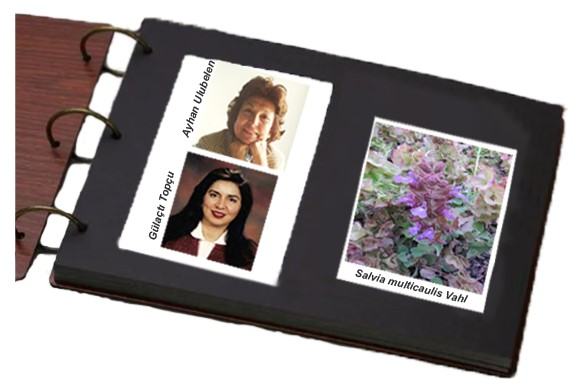
\includegraphics[width=12cm]{./pic/t1-1.jpg}
\end{figure}

在一篇关于\emph{Salvia multicaulis}Vahl.的研究中,Ulubelen和Topçu分离出了4种具有抗结核活性的全新芳香松香烷型二萜\textbf{1}--\textbf{4}。不仅分离出的二萜化合物具有抗细菌和抗真菌活性,植物提取物也显示出抗氧化、消炎和抑制胆碱酯酶的活性。\emph{S. multicaulis}在小亚细亚民间亦有使用,如作为开胃菜、用于促进伤口愈合,以及治疗蝎子叮咬、呼吸道感染、尿路感染和糖尿病等。

\begin{figure}[h]
	\centering
	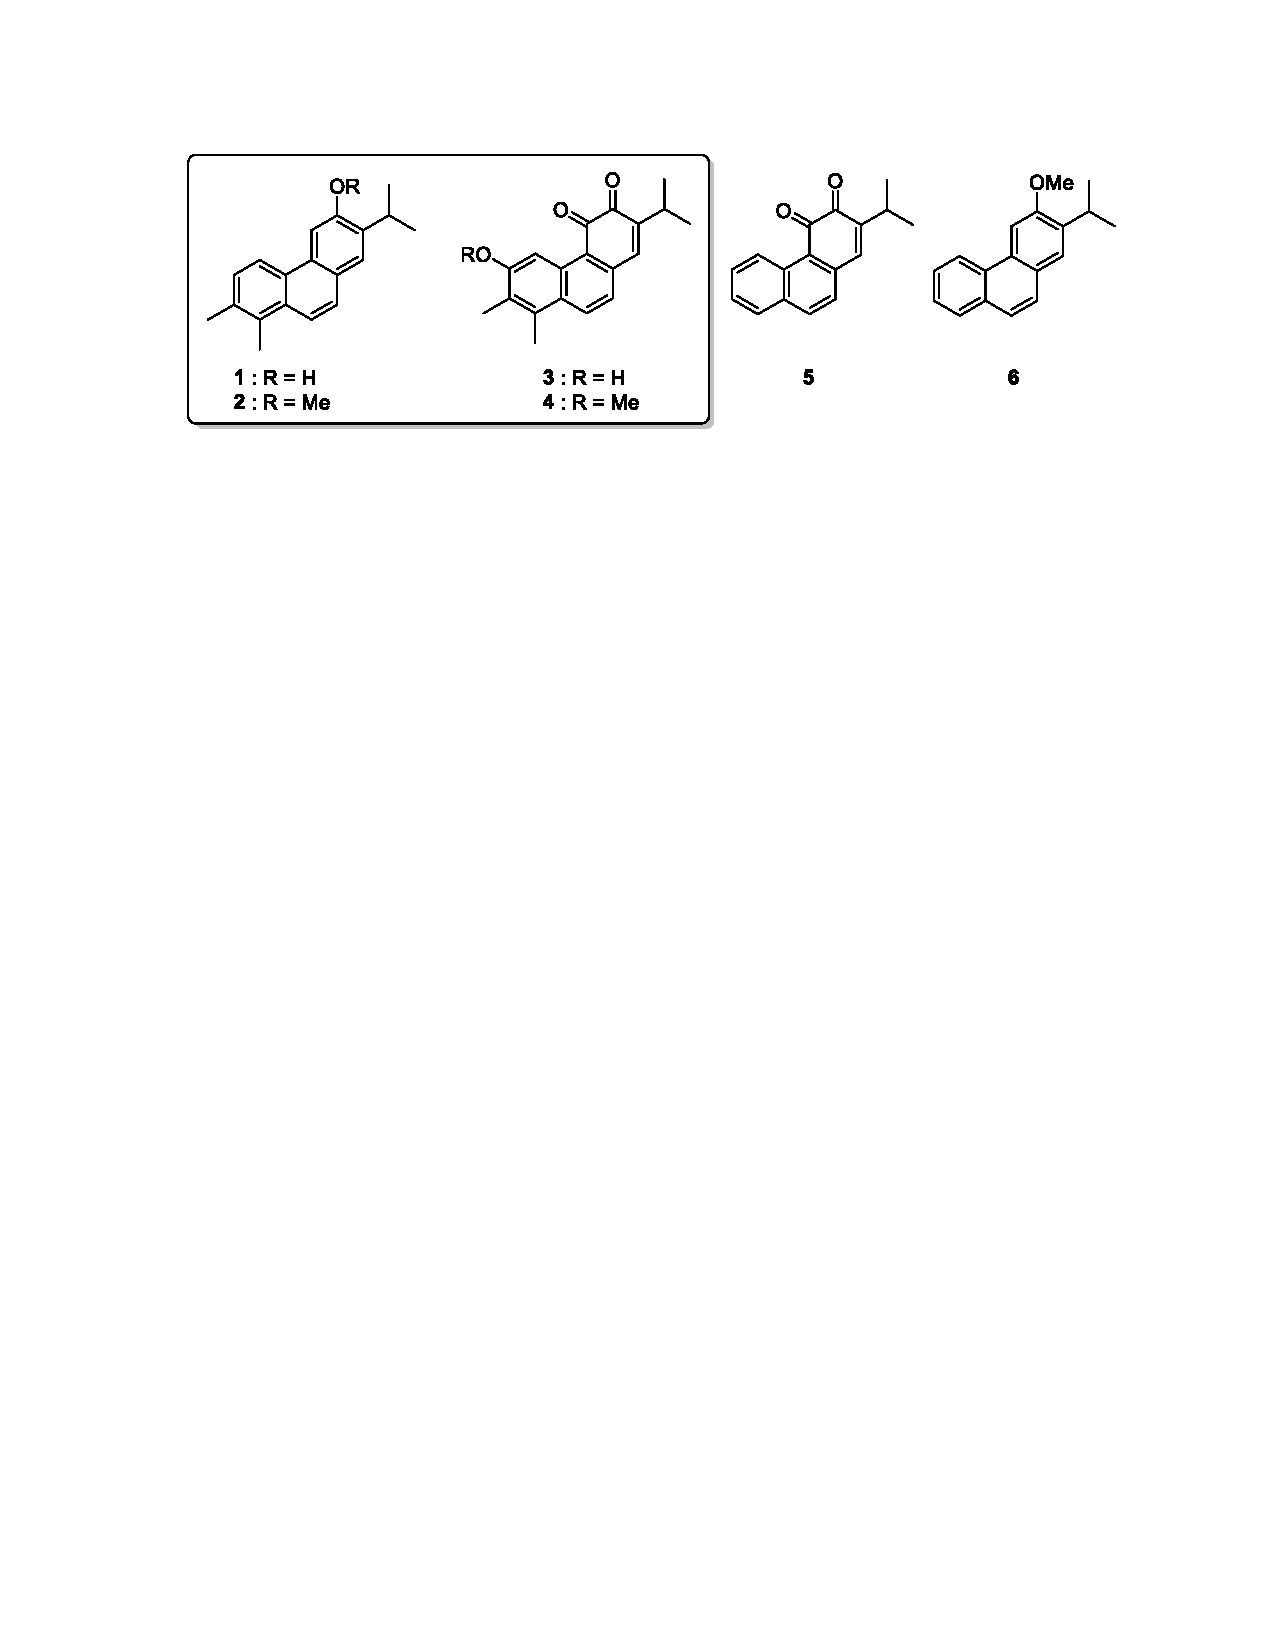
\includegraphics[width=14cm]{./pic/t1-2.pdf}
\end{figure}

随后一个土耳其的研究组发展了天然产物\textbf{1}--\textbf{4}衍生物的合成路线,本题就来源于此。合成二萜\textbf{1}和\textbf{5}的反应图如下所示。

\begin{figure}[h]
	\centering
	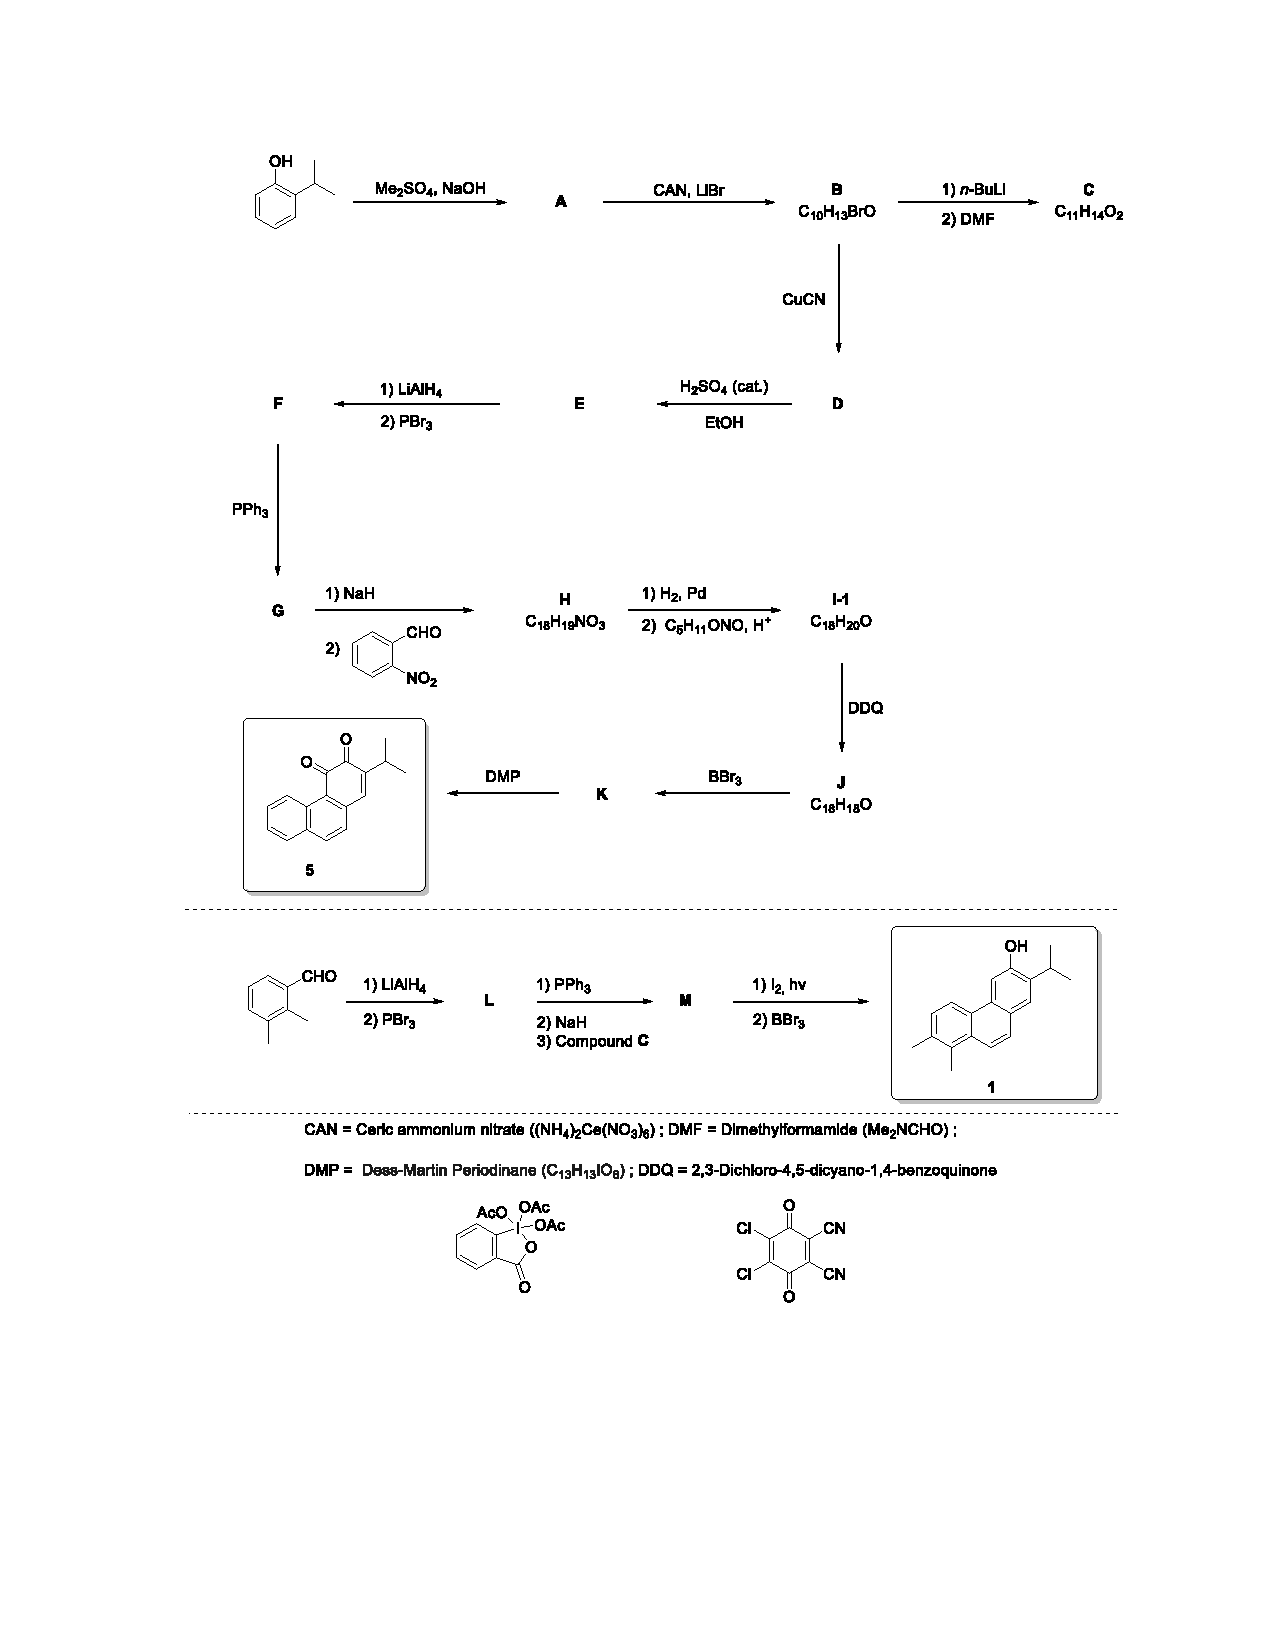
\includegraphics[width=16cm]{./pic/t1-3.pdf}
\end{figure}

\noindent\textbf{1.1.} 画出产物\textbf{A}--\textbf{M}的结构,无需考虑立体构型。\textbf{提示}:第二步 (\textbf{A}$\rightarrow$\textbf{B})中,溴化锂和硫酸铈(IV)铵合用作溴化试剂。化合物\textbf{C}是苯甲醛衍生物并用于化合物\textbf{M}的多步合成中。

\noindent\textbf{1.2.}\textbf{H}到\textbf{I1}的环化过程中同时生成了异构体\textbf{I2},其化学式为C\textsubscript{18}H\textsubscript{20}O。画出\textbf{I2}的结构。

\noindent\textbf{1.3.} 接下来的反应图与二萜\textbf{1}和\textbf{2}的去甲基衍生物\textbf{6}有关。画出产物\textbf{N}--\textbf{Y},无需考虑立体构型。\textbf{提示}:化合物\textbf{R}、\textbf{S}、\textbf{T}有酸性。化合物\textbf{V}到\textbf{W}的转化包含Robinson增环和一个可能的去甲酰化过程。

\noindent\textbf{1.4.} 化合物\textbf{V}到\textbf{W}的转化过程中,使用$\alpha$,$\beta$--不饱和酮的前体(例如$\beta$--氯代酮或\emph{N},\emph{N},\emph{N}--三烷基--3--氧代丁基卤化铵)更好。解释原因。

\noindent\textbf{1.5.} 画出化合物\textbf{V}可能的异构体。

\noindent\textbf{1.6.} 化合物\textbf{Y}也可由化合物\textbf{Z}经电环化关环得到。画出\textbf{Z}的结构。

\noindent\textbf{1.7.} 从\textbf{X}到\textbf{Y}的转化也可使用下列哪组试剂?(忽略S\textsubscript{N}2$'$反应)。

\begin{figure}[h]
	\centering
	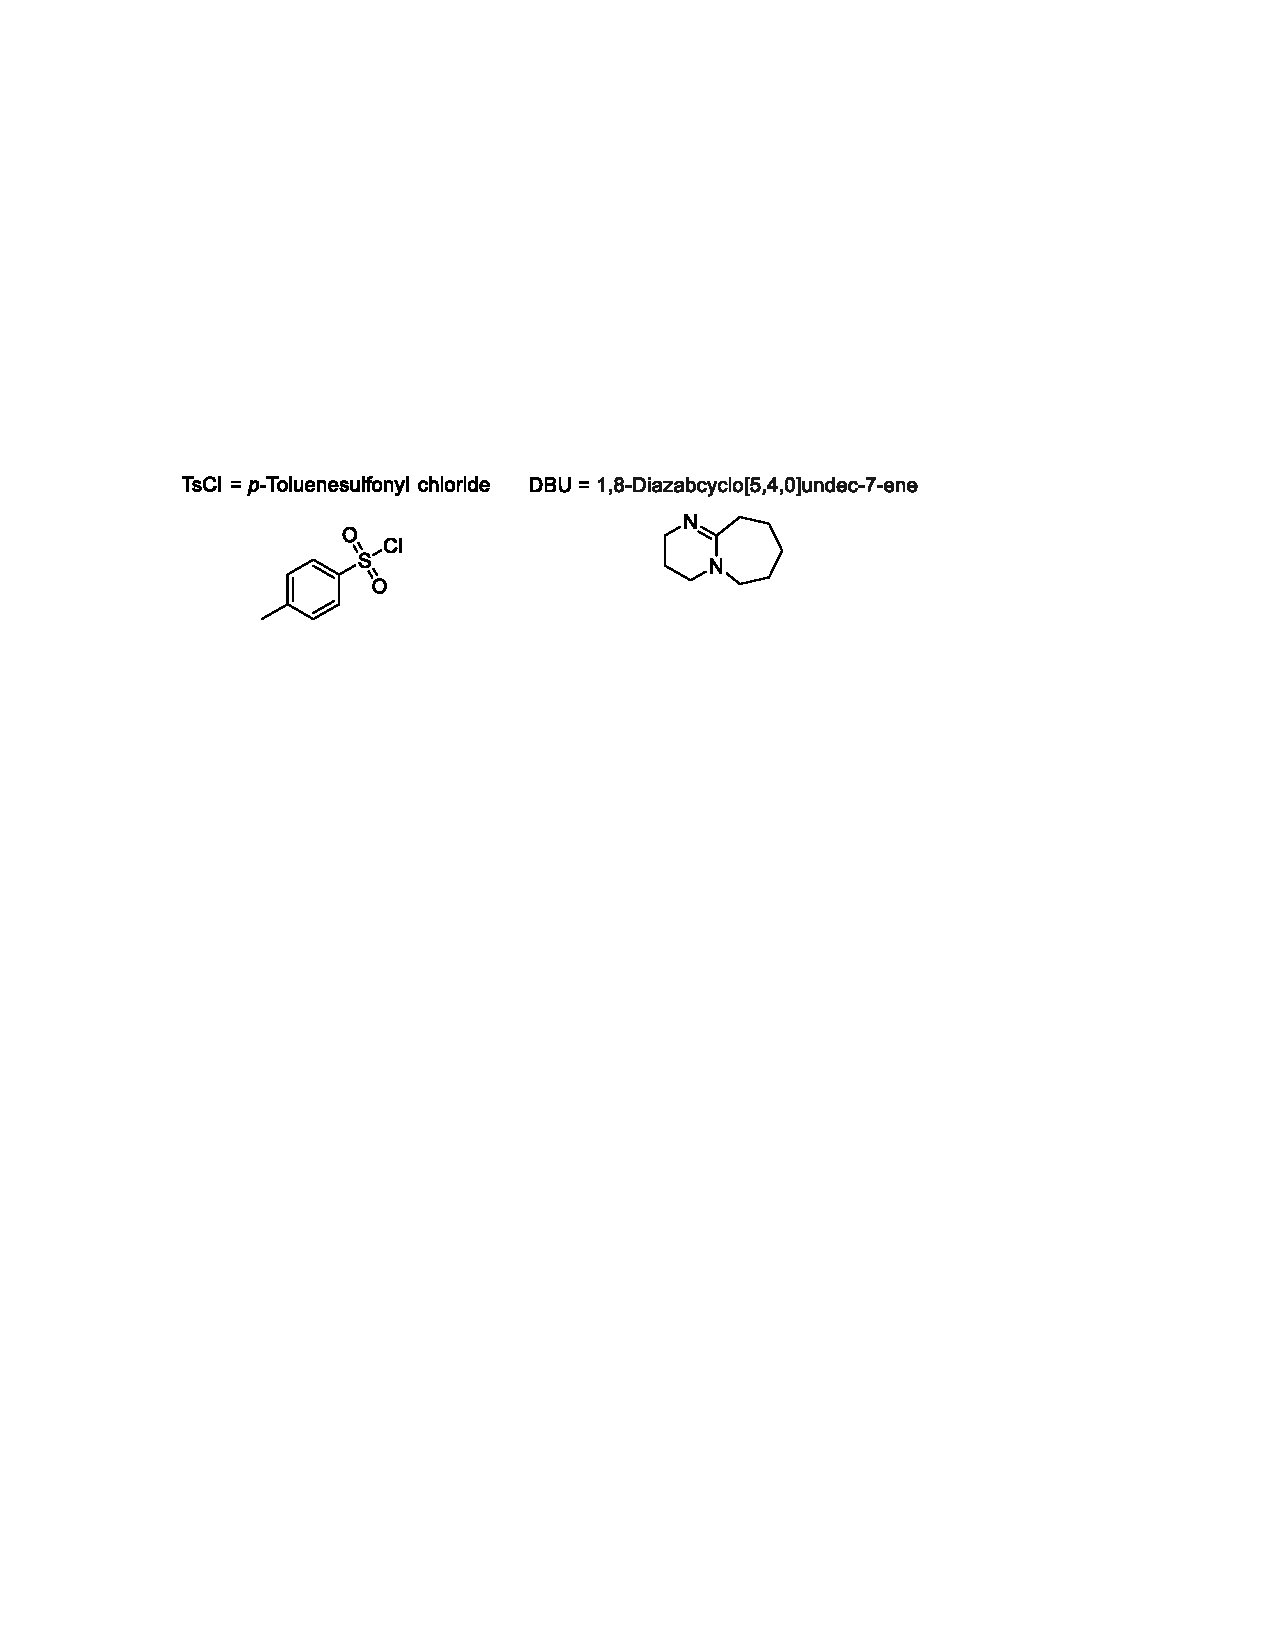
\includegraphics[width=12cm]{./pic/t1-5.pdf}
\end{figure}

\renewcommand{\labelitemi}{$\square$}
\begin{itemize}
	\item i) PBr\textsubscript{3}/吡啶; ii)  \textit{n}--Bu\textsubscript{3}SnH/AIBN
	\item i) PBr\textsubscript{3}/吡啶; ii) Na/\emph{t}--BuOH
	\item i) MnO\textsubscript{2}; ii) DDQ
	\item i) TsCl/吡啶; ii) LiAlH\textsubscript{4}
	\item TsCl/吡啶; ii) DBU
\end{itemize}
\renewcommand{\labelitemi}{$\bullet$}

\begin{figure}[h]
	\centering
	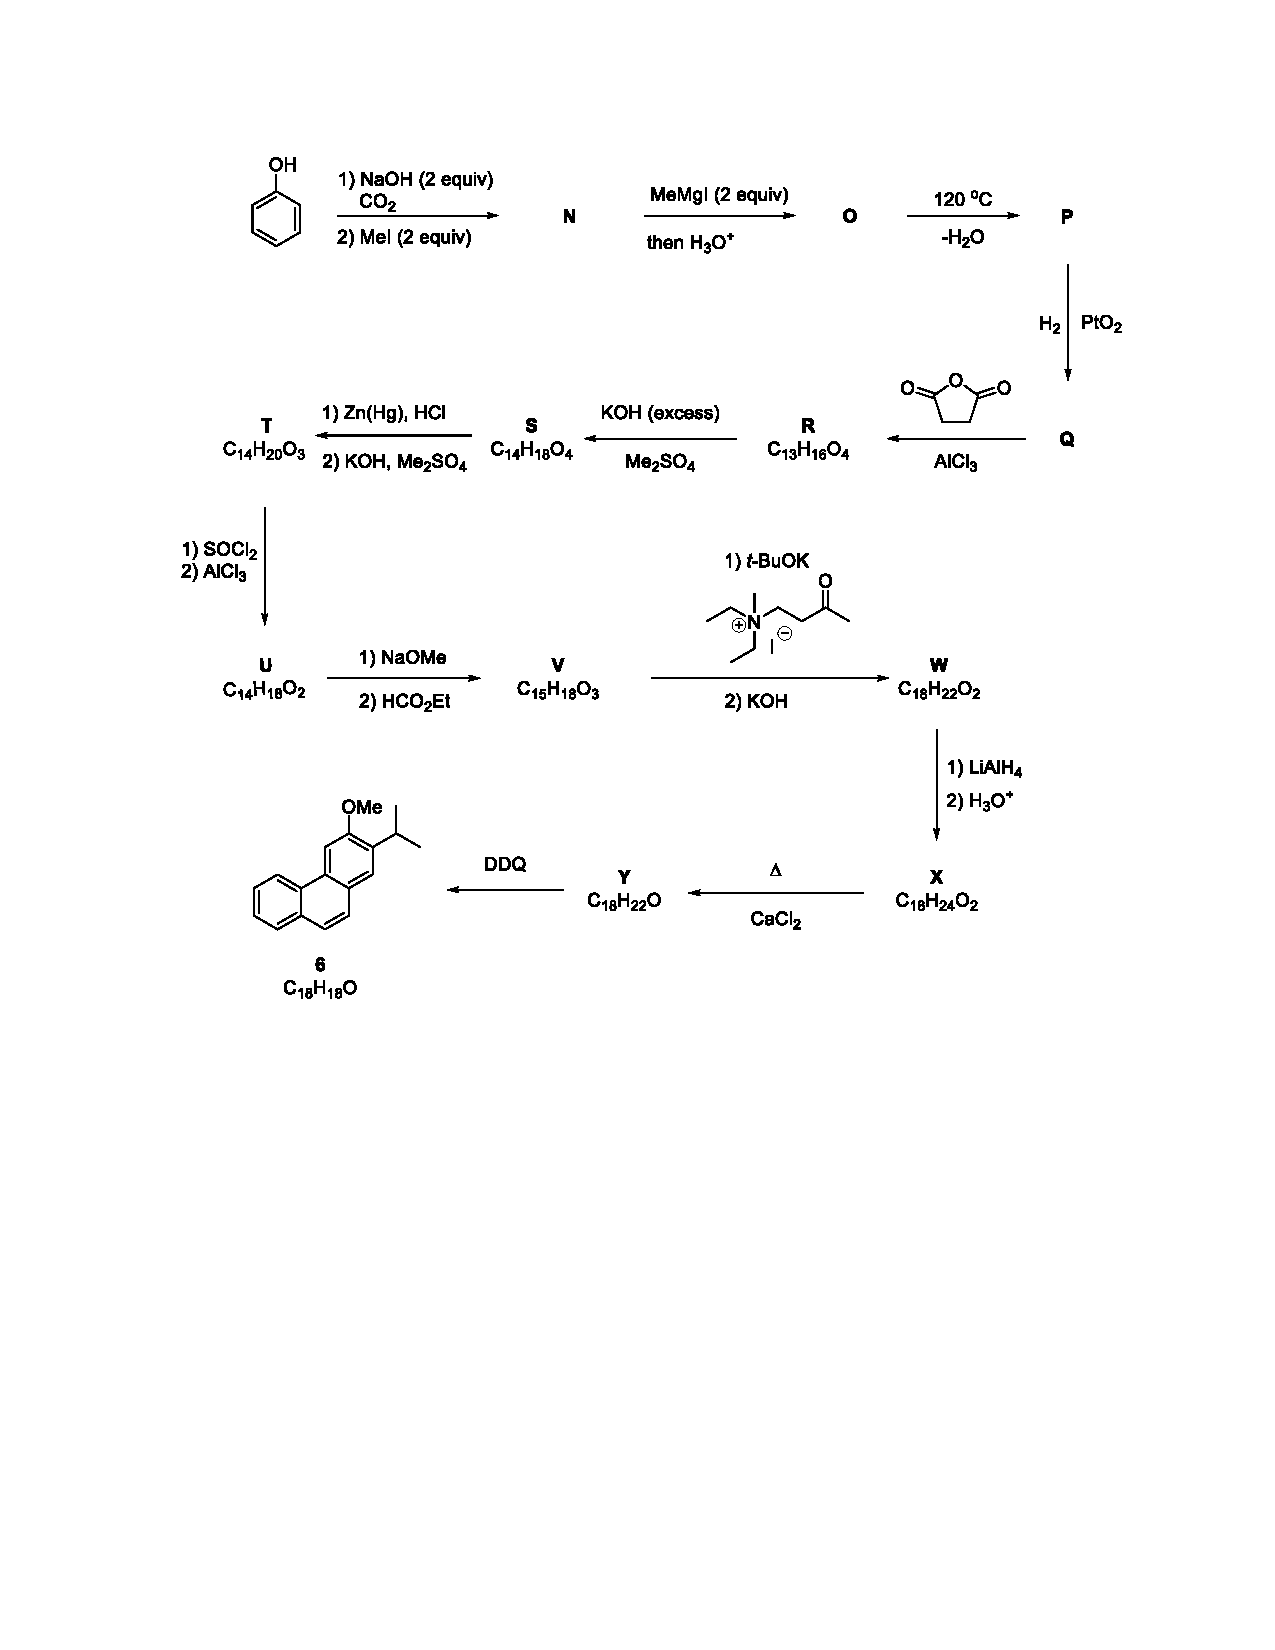
\includegraphics[width=15cm]{./pic/t1-4.pdf}
\end{figure}

\newpage
\mysection{第2题\  Istanbulin和相关的倍半萜天然产物}
\textbf{图}

一些元素的名字源于由世界各地的地名。这一点上,瑞典村庄Ytterby创造了一项纪录,四种元素:镱(ytterbium,Yb)、钇(yttrium,Y)、铒(erbium,Er)和铽(terbium,Tb)得名于此。然而,并不仅仅是元素会以地名命名。有趣的是,一系列天然产物\textbf{istanbulin A--E}的名字源于城市伊斯坦布尔。这一系列的前两个成员即istanbulin A和B首次于1971年由教授Ayhan Ulubelen博士及其合作者从植物\emph{Smyrnium olusatrum}(译注:又名亚历山大草)中分离得到。剩下的3个成员即istanbulin C--E由Ulubelen及其合作者在1979年至1982年间报道。

\textbf{图}

Istanbulin是倍半萜天然产物这一更大家庭中的一员。Vernolepin \textbf{1}和vernomenin \textbf{2}是两种重要的倍半萜天然产物,它们具有类似的6-6-5并环体系。1976年,Danishefsky及其合作者报道了这两个化合物的全合成。在这一漂亮的全合成路线中,Danishefsky将所谓Danishefsky二烯用于Diels--Alder (DA)反应中。

请注意本题中所有的手性化合物的结构式都表示外消旋体。

\textbf{图}

上下文中提到的Danishefsky二烯 \textbf{3}和Rawal--Kozmin二烯 \textbf{4}是两个富电子二烯,都已广泛用于有机合成中。它们的结构如下所示:

\textbf{图}

TMS: 三甲基硅基;TBS: 叔丁二甲基硅基

\noindent\textbf{2.1.}画出\textbf{3}和\textbf{4}主要的共振式。指出每个二烯中电子密度最高的碳原子。

\noindent\textbf{2.2.}化合物\textbf{3}和\textbf{4}广泛用作Diels--Alder反应的双烯体。画出\textbf{3}和\textbf{4}能够发生DA反应时的构象。推测在与顺丁烯二酸酐发生DA反应时,哪个二烯的活性更高?

加热Danishefsky二烯 \textbf{3}与化合物\textbf{6}的混合物,随后用酸(TsOH,对甲苯磺酸)处理,得到主要产物化合物\textbf{A}。

\noindent\textbf{2.3.}画出\textbf{3}和\textbf{6}发生Diels--Alder反应所有可能的产物,它们的化学式都为C\textsubscript{12}H\textsubscript{14}O\textsubscript{3}。每一组对映异构体画出其中一种即可。

\textbf{图}

\noindent\textbf{2.4.} 确定主产物\textbf{A}的结构。

\noindent\textbf{2.5.} Diels--Alder加合物\textbf{A}依次经历如下的4步反应转化为化合物\textbf{7}。化合物\textbf{B}具有酸性。画出\textbf{B}-\textbf{D}的结构。

\textbf{图}

\noindent\textbf{2.6.} 化合物\textbf{7}与1当量\emph{m}-CPBA反应得到主产物\textbf{E}。圈出与\emph{m}-CPBA选择性发生反应的官能团,画出\textbf{E}的结构。

\noindent\textbf{2.7.} Vernolepin \textbf{1} 和 vernomenin \textbf{2}的全合成经如下步骤完成。画出化合物\textbf{F}-\textbf{J}的结构。最后一步中,化合物\textbf{I}是\textbf{1}的前体。

\textbf{图}

\newpage
\mysection{第3题\  茶,荼,檟,蔎,茗,荈和格雷伯爵茶之味:香柠檬}
一曰茶,二曰檟,三曰蔎,四曰茗,五曰荈

\begin{flushright}
------陆羽 《茶经》
\end{flushright}

茶(土耳其语:çay)流行于土耳其以及海外土耳其人中。土耳其茶文化同时影响了阿塞拜疆在内的巴尔干半岛诸国。土耳其的人均茶消耗量世界第一,达到2.5
kg/人/年,紧随其后的是英国(2.1 kg/人/年)。

香柠檬烯(bergamotene)及其衍生物\textbf{1}-\textbf{4}属倍半萜类化合物,皆为蒎烷类单萜的类似物。香柠檬烯存在于香柠檬油中,是格雷伯爵茶香和味的来源。

\begin{figure}[h]
	\centering
	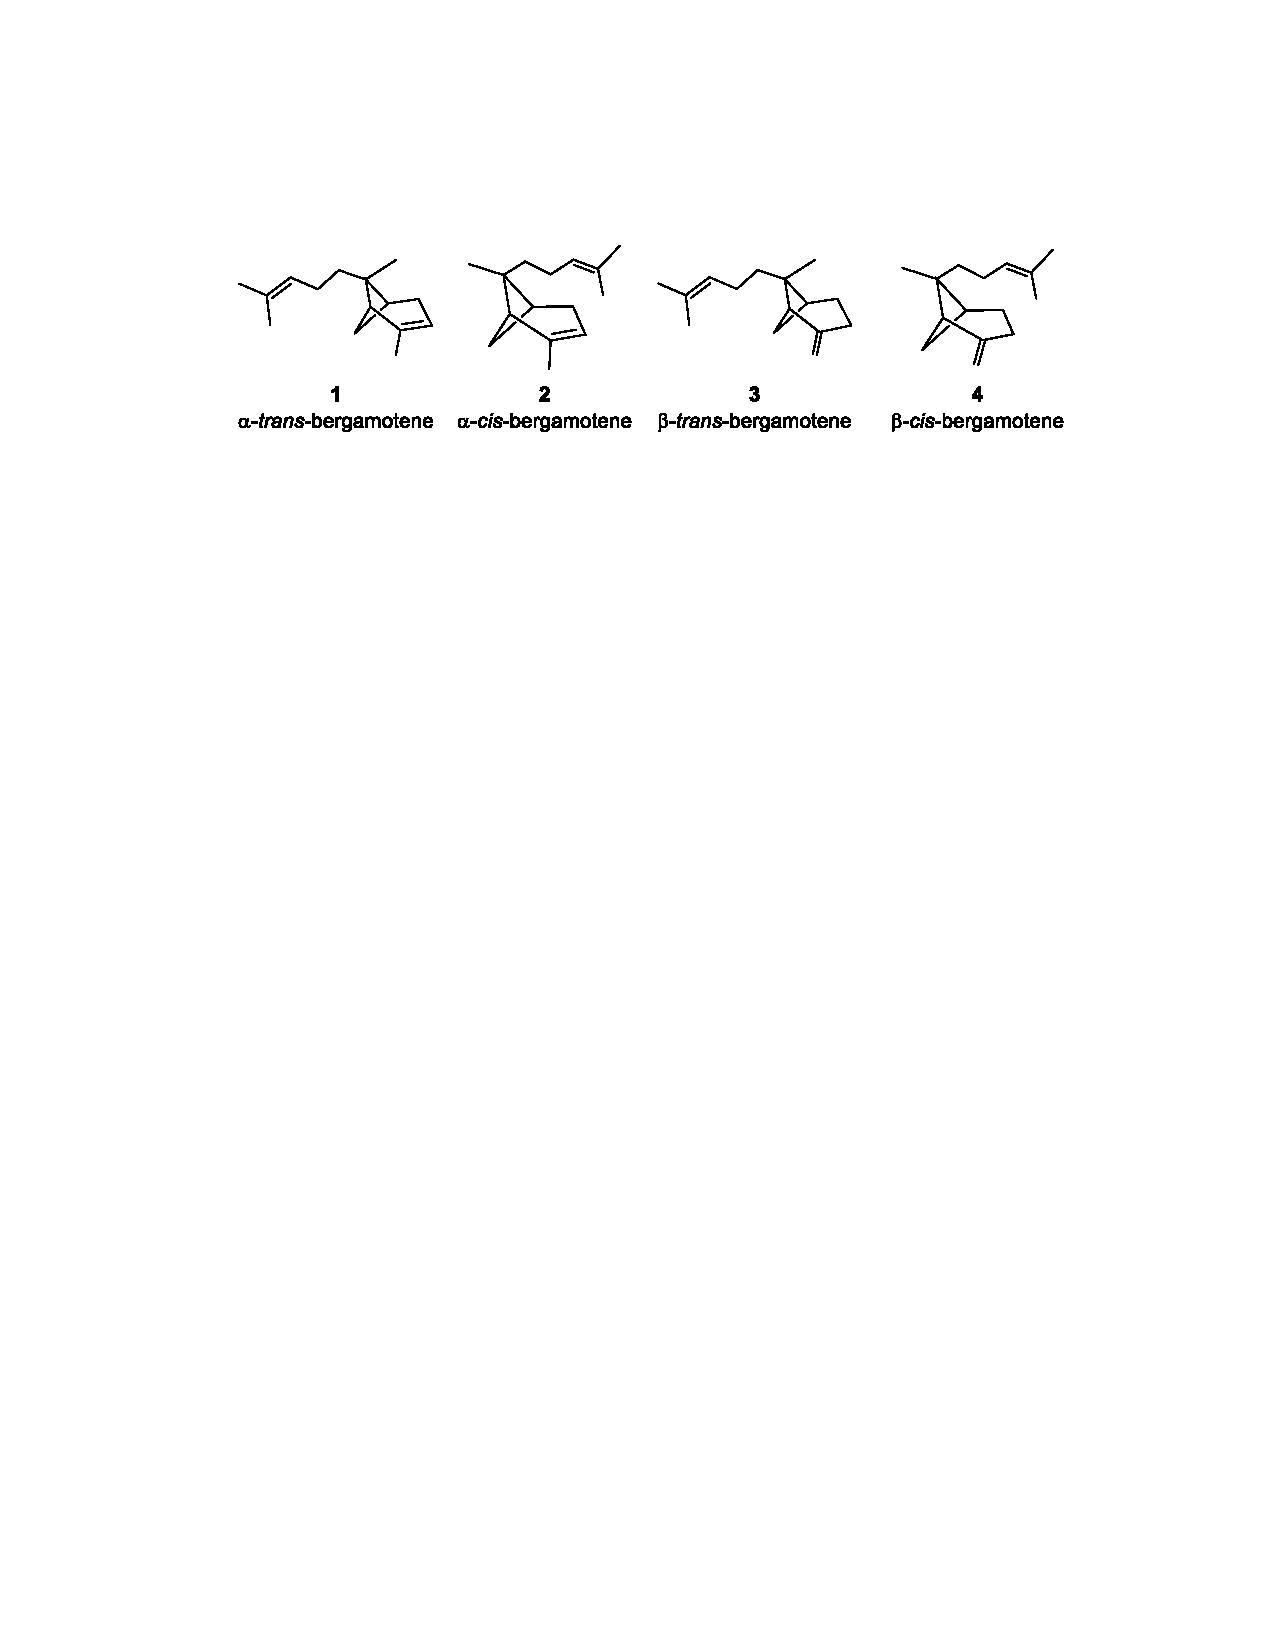
\includegraphics[width=13cm]{./pic/t3-1.pdf}
\end{figure}

\noindent\textbf{3.1.}以下的反应图示出了$\alpha$-反式香柠檬烯\textbf{1}的合成路线。画出产物\textbf{A}-\textbf{G}的结构。

\noindent\textbf{3.2.} 从\textbf{A}到\textbf{B}的转化中,试剂Me\textsubscript{3}NO的作用是什么?

\begin{figure}[h]
	\centering
	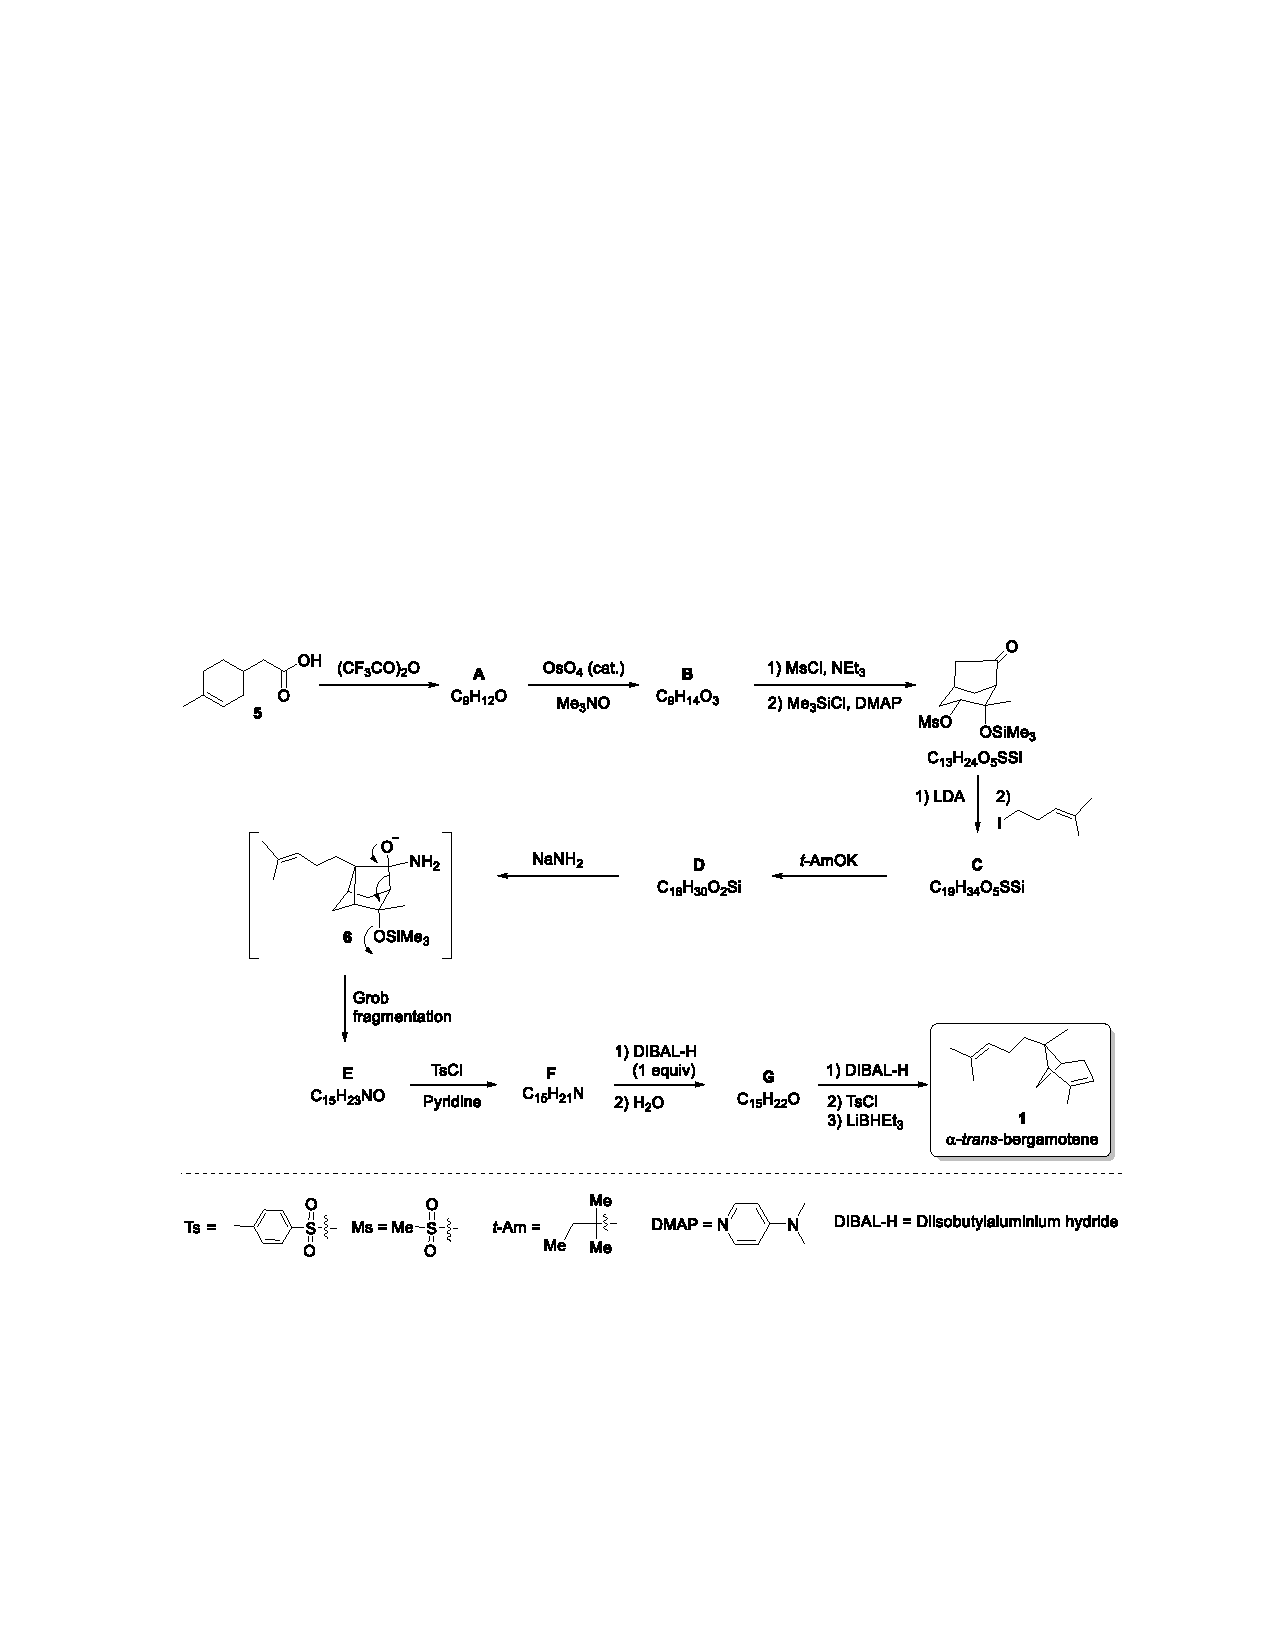
\includegraphics[width=16cm]{./pic/t3-2.pdf}
\end{figure}


\newpage
\mysection{第4题\  马氏规则和俄国近现代有机化学家}
马氏规则由俄罗斯化学家马尔科夫尼科夫(Vladimir V.Markovnikov)在1869年提出,而2019年是马氏规则被提出的第150周年。马尔科夫尼科夫是俄罗斯著名科学家布特列洛夫(Alexander Butlerov)的博士生。在他1869年发布的博士论文中,马尔科夫尼科夫提出了几乎每本现今有机化学教科书中都有引用的马氏规则,其指出:当不对称的烯烃或炔烃与卤化氢(包括氯化氢、溴化氢及碘化氢)发生加成反应时,卤化氢中的氢原子加在含氢较多的碳原子上。但是在某些情况中,由于底物和试剂的不同,与上述结论相反的实验结果也被观察到,这种相反的结果被称作反马氏加成。虽然马氏规则是针对卤化氢对烯烃和炔烃的加成反应而提出的,但随着有机化学的发展,许多其它的加成反应因选择性相似而也被相应描述为马氏或反马氏规则。

事实上,马氏规则应该被修改为:对碳碳双键和三键的加成选择性来自于更加稳定的中间体的形成。在某些情况下,除了电子效应之外,空间效应也会影响马氏或反马氏加成产物的比例。

以下问题主要与著名化学家布特列洛夫和他在喀山大学的同事及学生们的各类研究发现有关。

\noindent\textbf{4.1.}
画出下列反应主要产物\textbf{A}-\textbf{E}的结构,注意立体化学(不考虑光学异构)。

\begin{figure}[h]
	\centering
	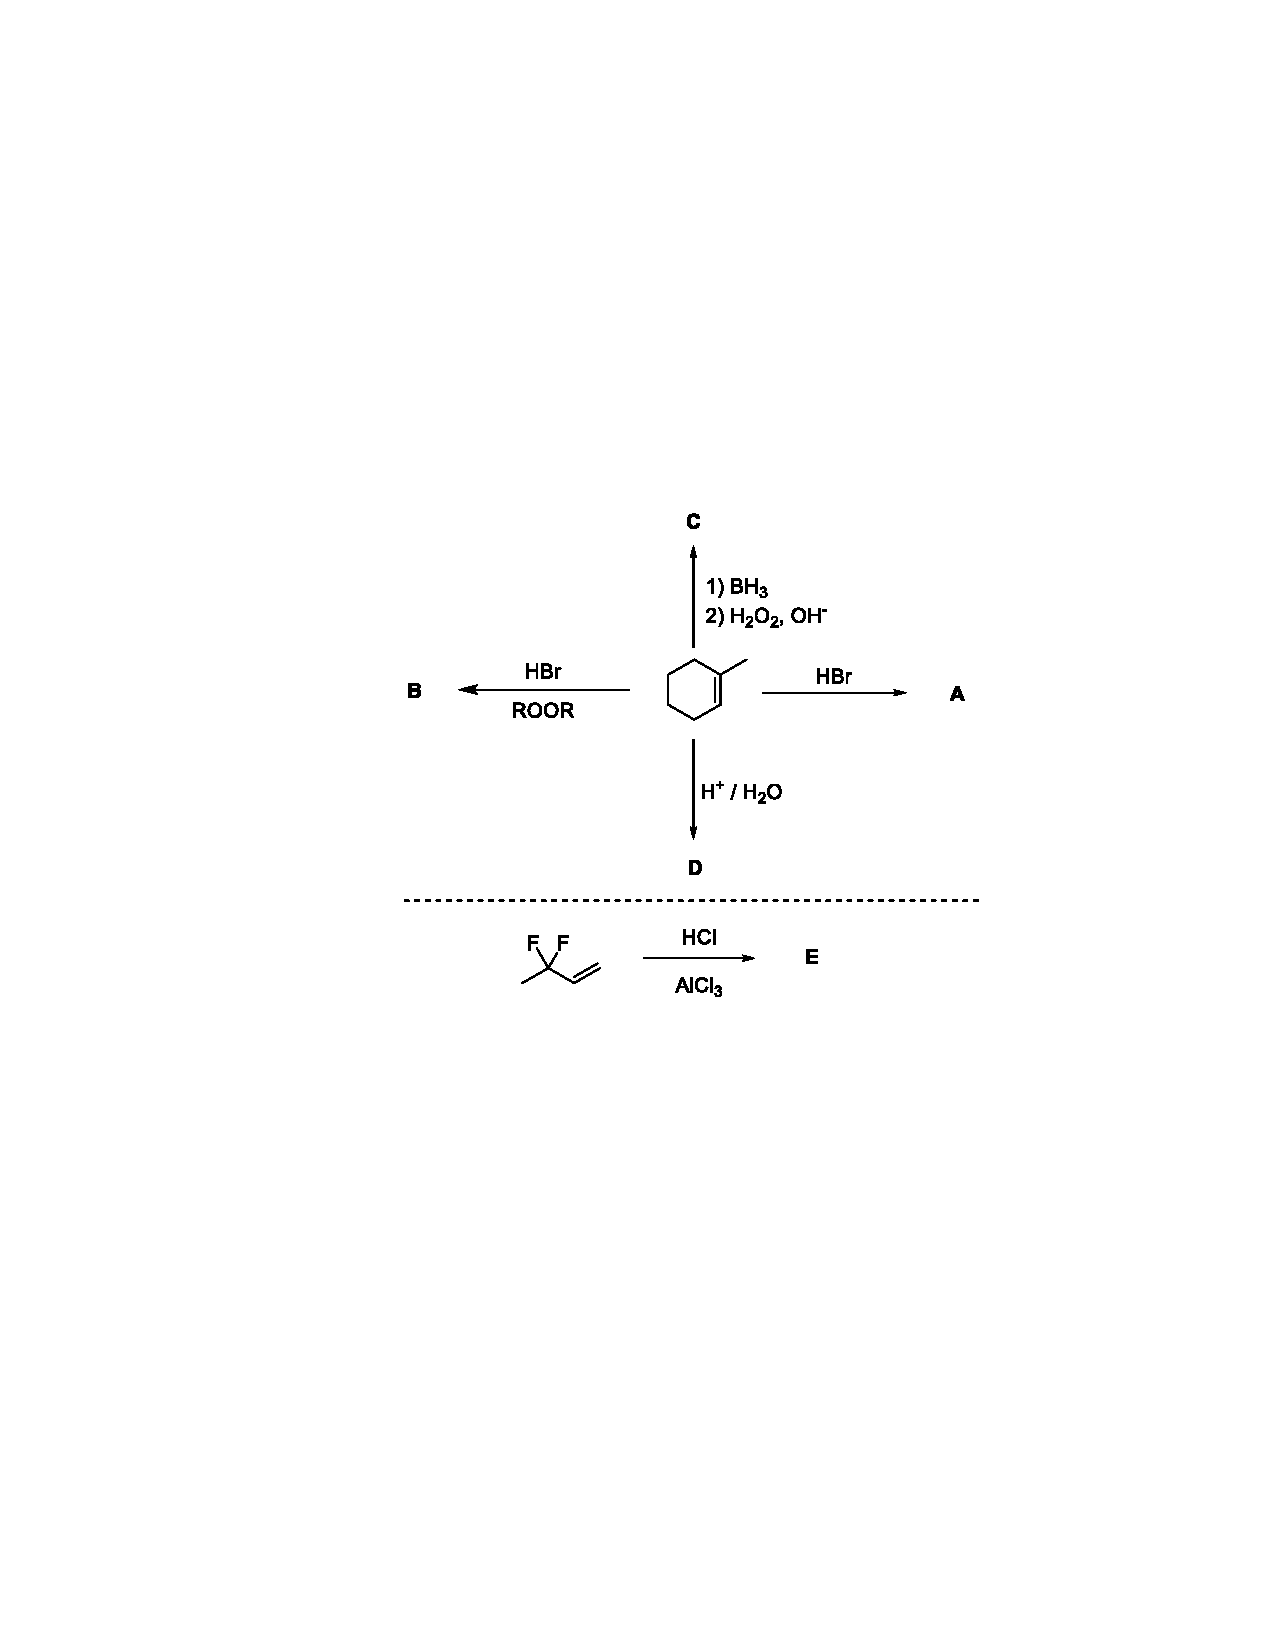
\includegraphics[width=10cm]{./pic/t4-2.pdf}
\end{figure}

\noindent\textbf{4.2.} 画出下列反应的主要产物\textbf{F}和\textbf{G}的结构。

\begin{figure}[h]
	\centering
	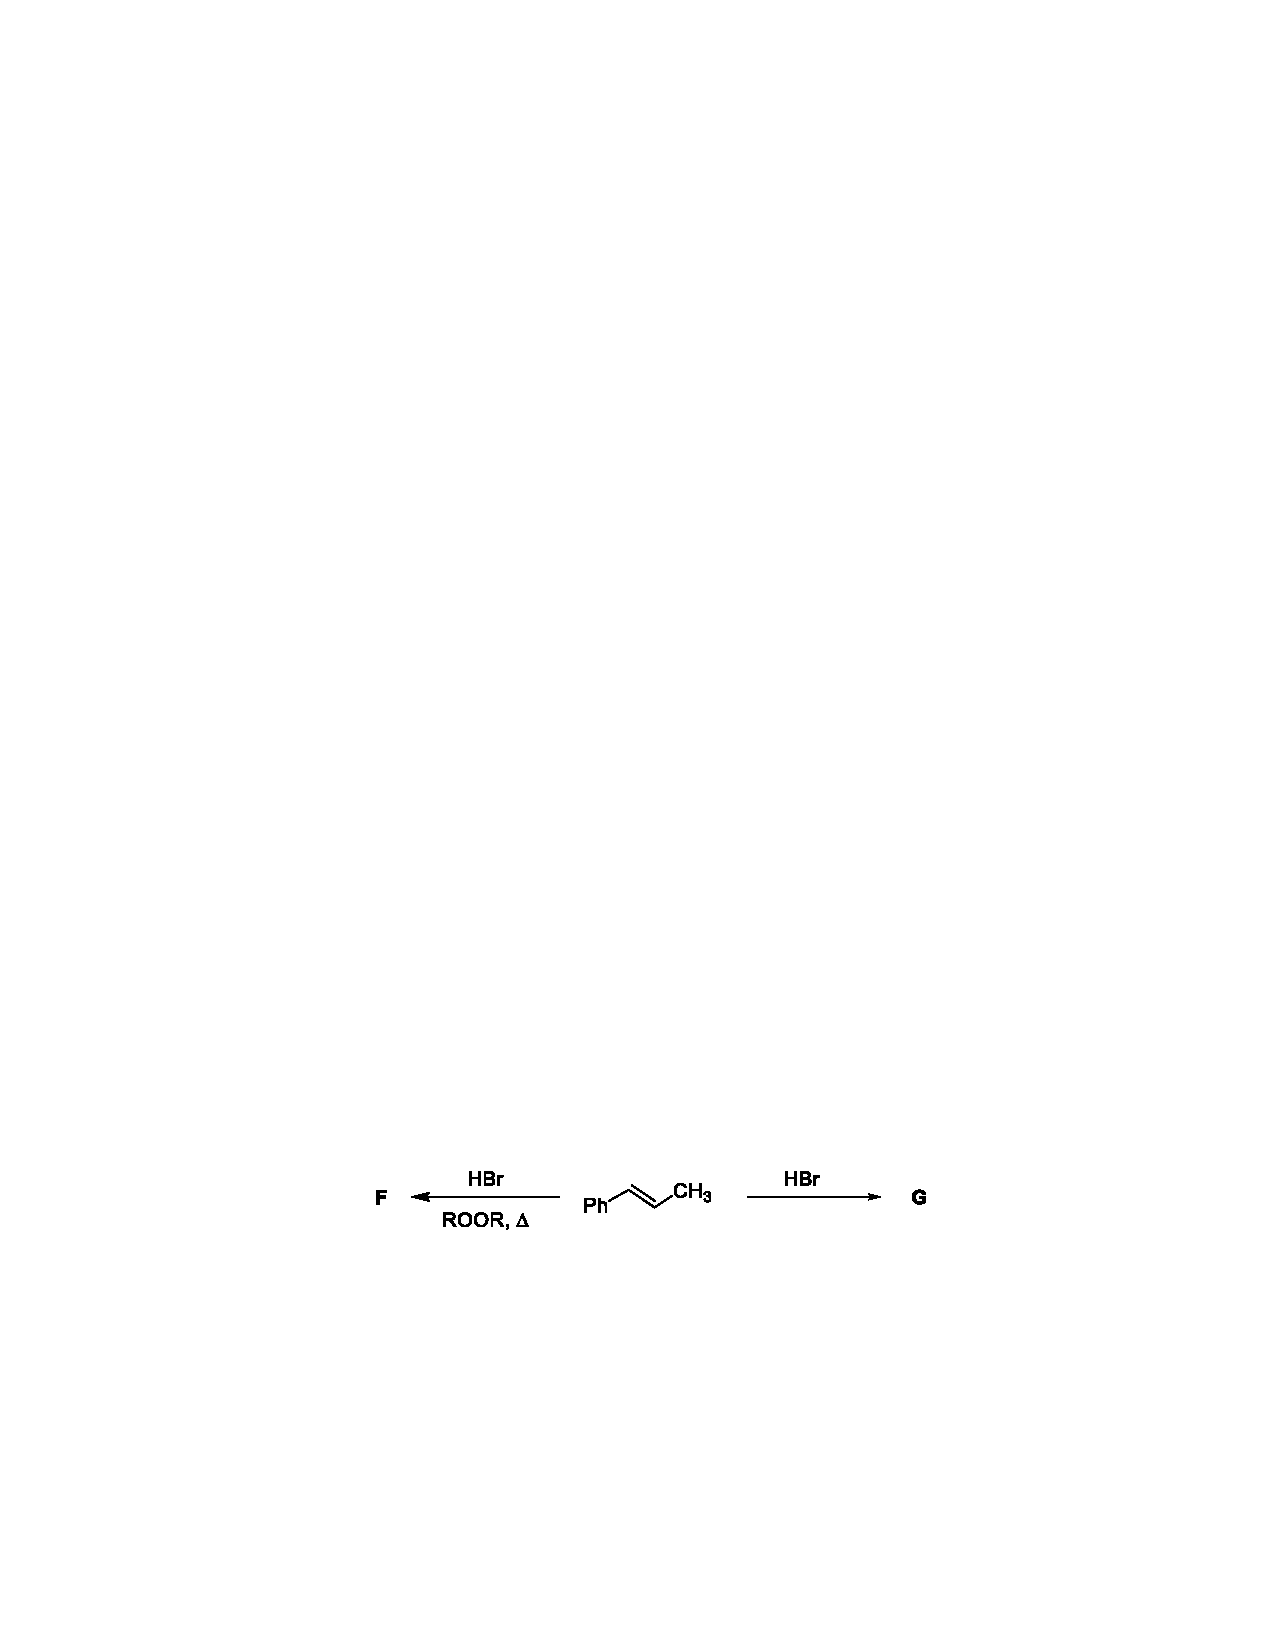
\includegraphics[width=10cm]{./pic/t4-3.pdf}
\end{figure}

\noindent\textbf{瓦格纳-梅尔外因重排反应(Wagner-Meerwein Rearrangement,WMR)}

瓦格纳是与布特列洛夫和马尔科夫尼科夫一同在喀山大学工作的另一位著名科学家。瓦格纳认为冰片基氯(2-氯-1,7,7-三甲基双环{[}2.2.1{]}庚烷)通过一个分子内的重排反应生成了蒎烯。梅尔外因随后推广了这类反应。因此,这类反应便被称作瓦格纳-梅尔外因重排反应。这类反应会在有碳正离子中间体生成时发生。一般来说,一个碳正离子会重排为一个更稳定的碳正离子,如果可能的话还会经过邻基参与的过程。此外,如果一个反应不经历碳正离子或类似中间体的历程,重排反应便不会发生。

\begin{figure}[h!]
	\centering
	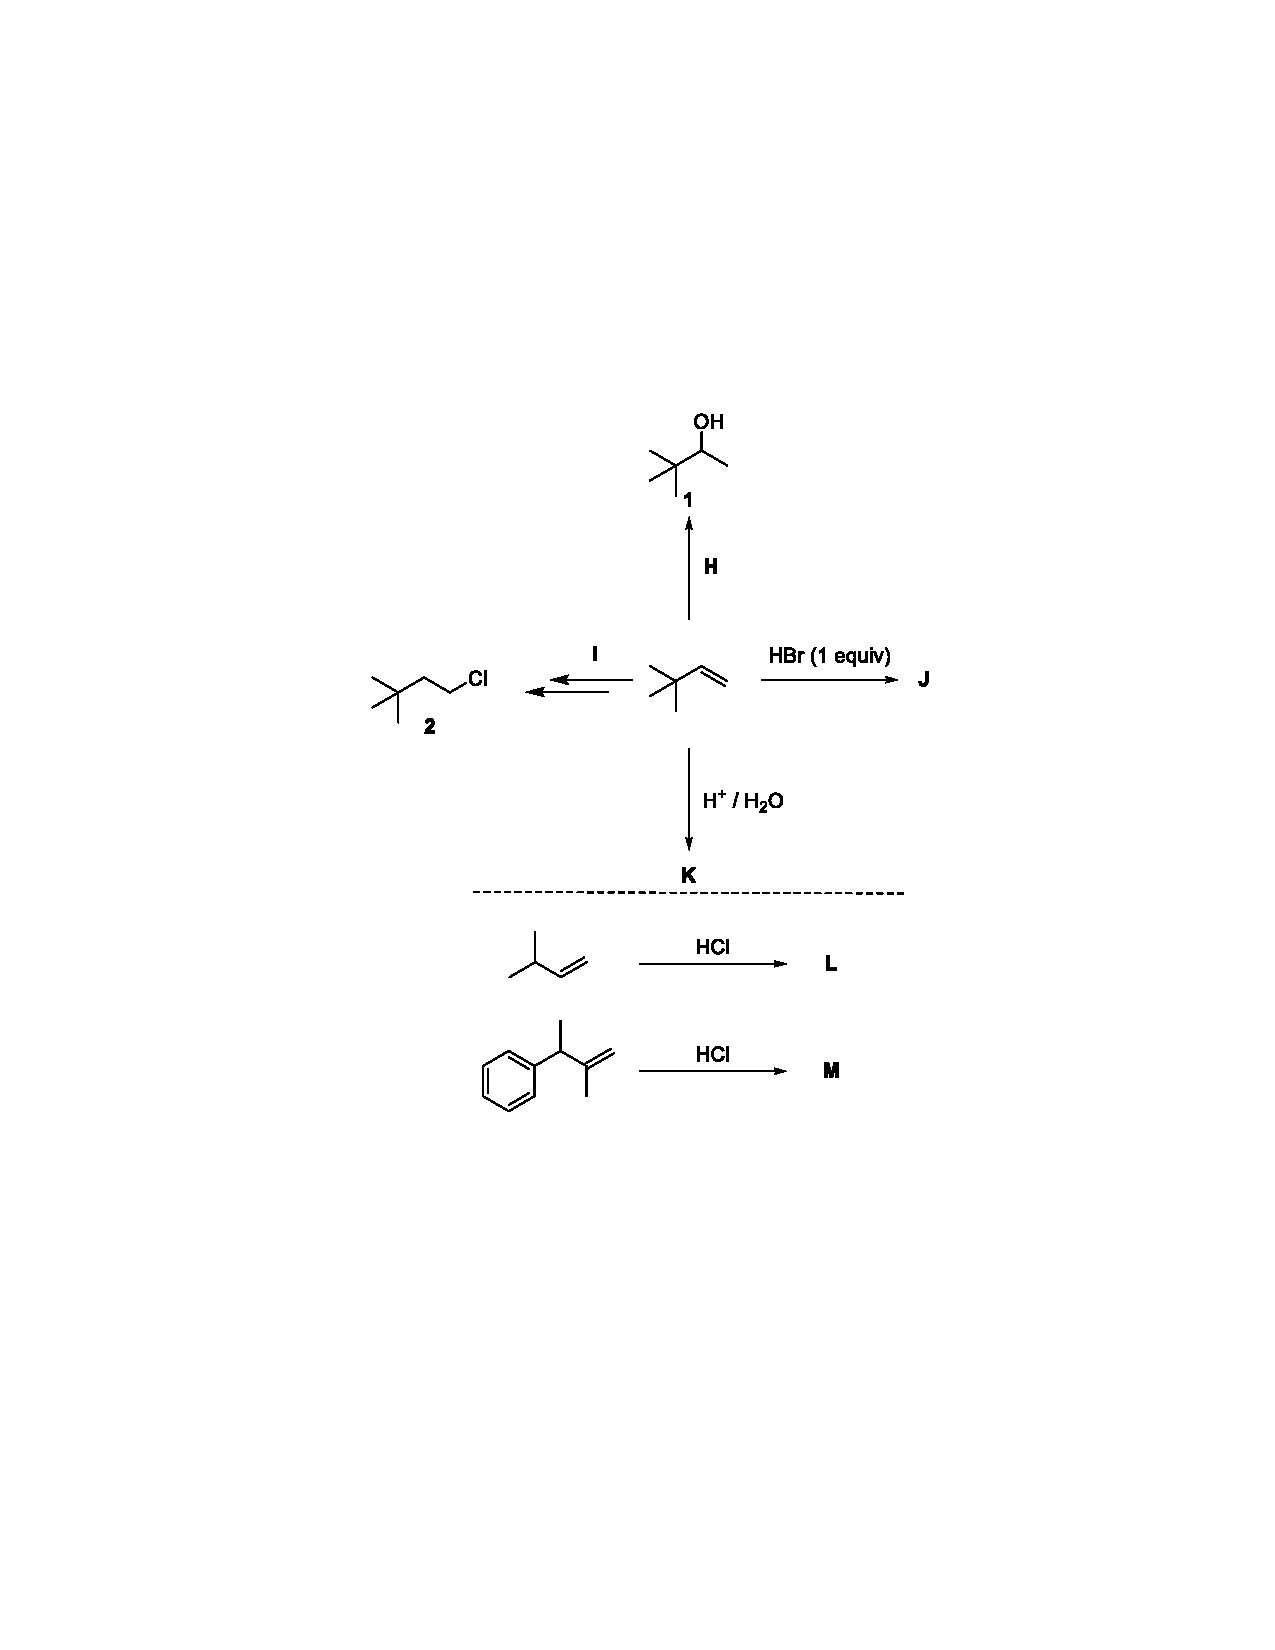
\includegraphics[width=10cm]{./pic/t4-4.pdf}
\end{figure}

\noindent\textbf{4.3.}
充分考虑每个反应过程中生成的中间体,画出试剂\textbf{H}和\textbf{I,}以及主要产物\textbf{J-M}的结构。

\noindent\textbf{酸催化的瓦格纳-梅尔外因重排}

4,4-二甲基环己-2,5-二烯-1-酮在酸催化下反应生成化合物\textbf{N}。其NMR谱图如下所示。

\begin{figure}[h!]
	\centering
	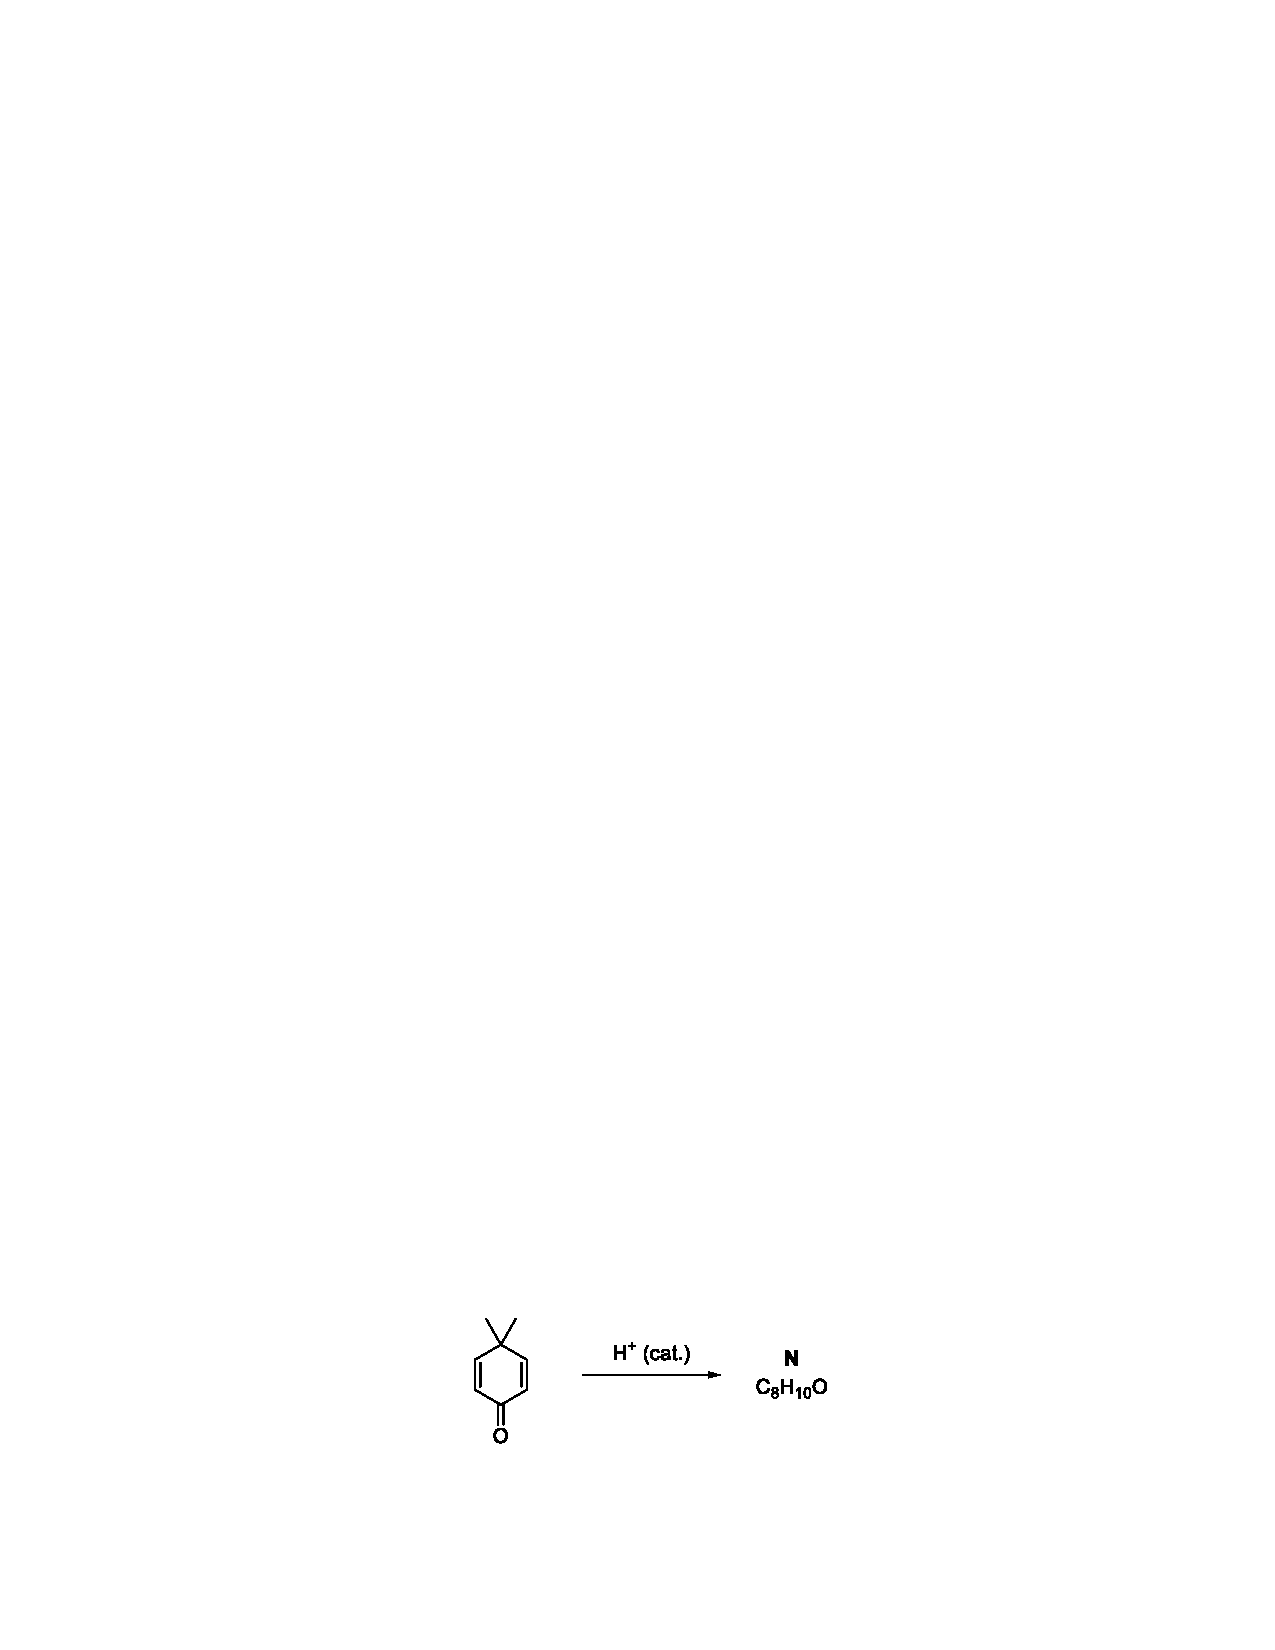
\includegraphics[width=7cm]{./pic/t4-5.pdf}
\end{figure}

For \textbf{N}; \textsuperscript{1}H NMR (300 MHz, CDCl\textsubscript{3}): δ = 6.95 (d,
\emph{J} = 8.0 Hz, 1H), 6.61 (d, \emph{J} = 2.8 Hz, 1H), 6.57(dd, \emph{J} = 8.0, 2.8 Hz, 1H), 5.39 (bs, 1H), 2.16 (s, 3H), 2.14 (s,
3H). \textsuperscript{13}C NMR (100 MHz, CDCl\textsubscript{3}):δ 153.4, 137.9, 130.4, 128.6, 116.6, 112.3, 19.8, 18.7.

\noindent\textbf{4.4.} 推断化合物\textbf{N}的结构并推测合理的机理。

\noindent\textbf{4.5.} 推测当一滴D\textsubscript{2}O加入NMR管的溶剂中后在
\textsuperscript{1}H NMR谱中会出现什么变化?

\noindent\textbf{扎伊采夫规则(Zaitsev's Rule)}

扎伊采夫是化学家布特列洛夫的另一个博士生,并且也提出了一个由他的名字命名的规则------扎伊采夫规则(Zaitsev's or Saytzeff's or Saytzev's rule)。扎伊采夫规则是一个用以预测烯烃消除反应生成的优势产物的经验规则。在喀山大学,扎伊采夫研究了大量的消除反应,观测并总结了烯烃消除反应选择性的一般规律。更一般地说,扎伊采夫规则指出,在消除反应中优先生成最多取代的烯烃产物。接下来的问题主要与扎伊采夫规则有关。

\noindent\textbf{4.6.}
画出消除产物\textbf{O-Q}以及化合物\textbf{R}的结构。将\textbf{R}加热后生成的主要产物是什么?

\begin{figure}[h]
	\centering
	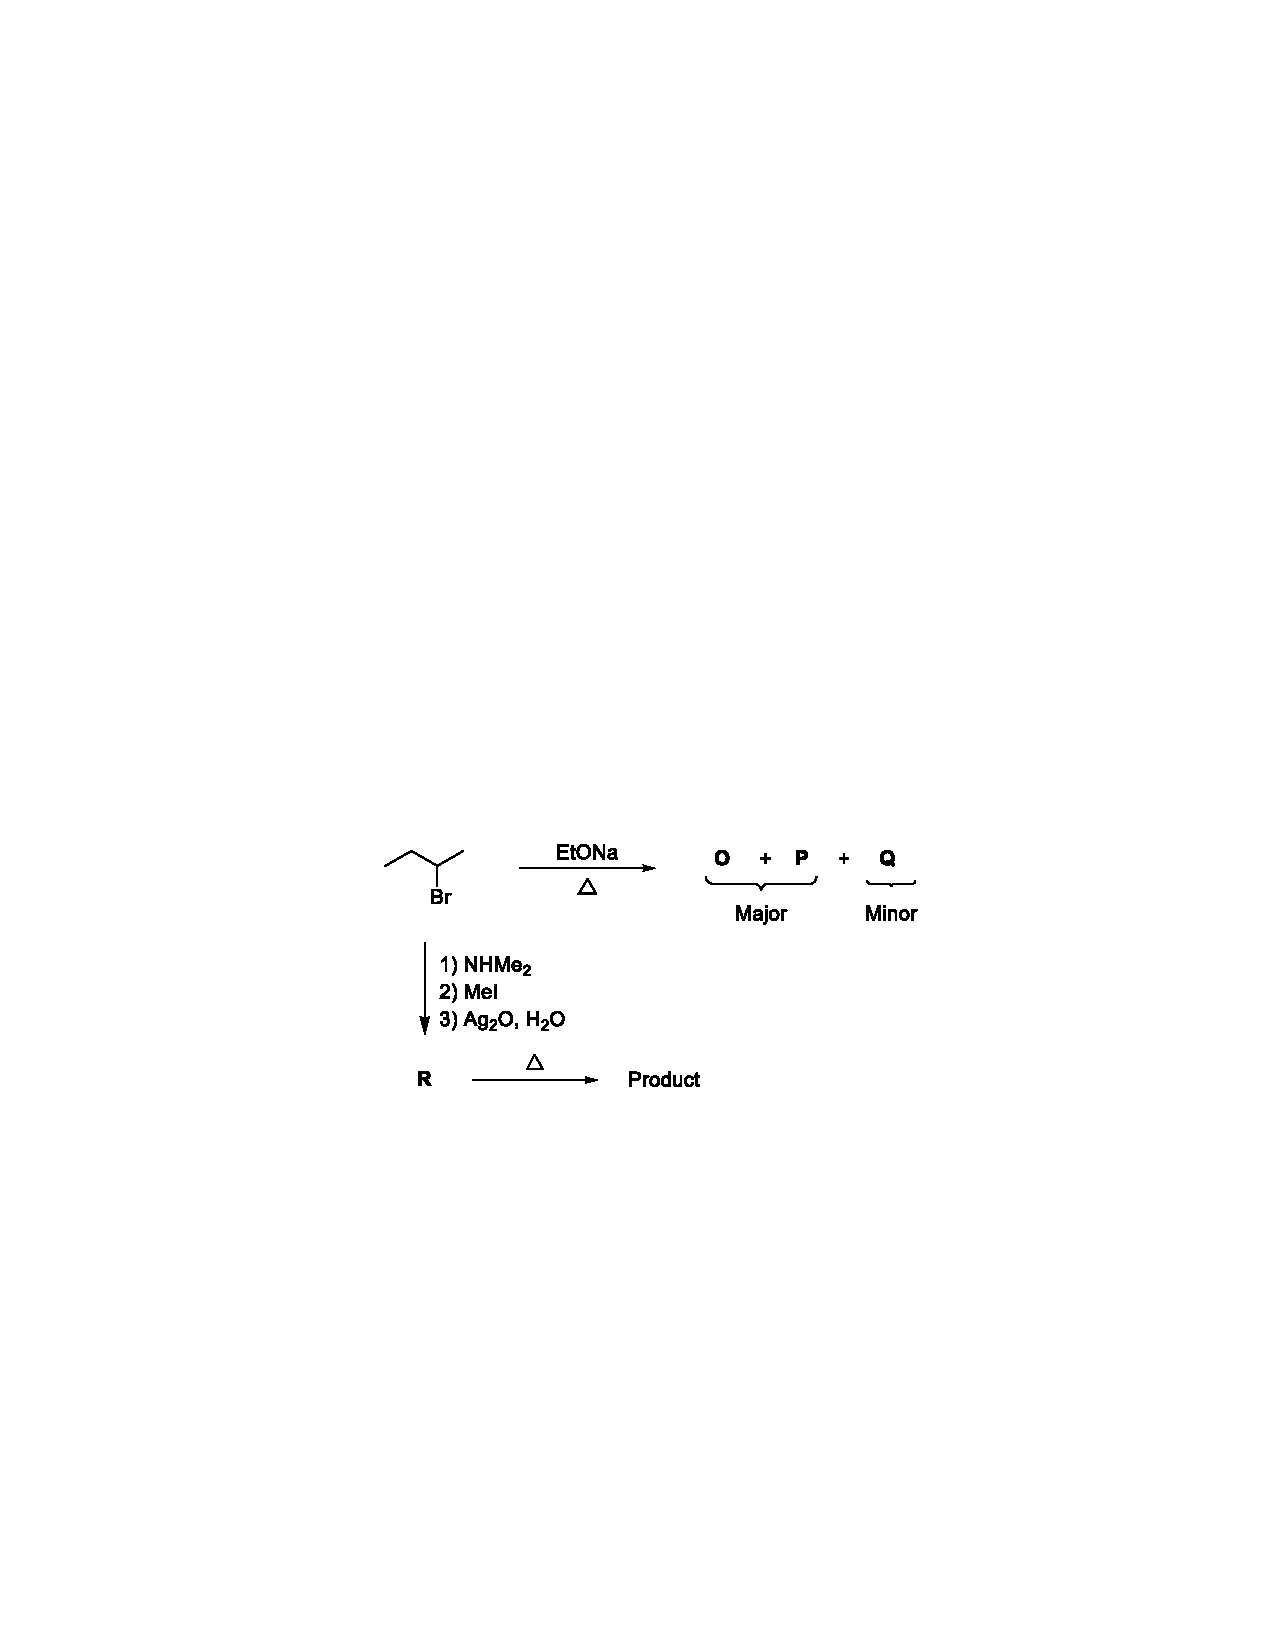
\includegraphics[width=10cm]{./pic/t4-6.pdf}
\end{figure}

\noindent\textbf{4.7.}
与EtONa相比,下列碱中哪个或哪些可以增加生成产物\textbf{Q}的比例?

\renewcommand{\labelitemi}{$\square$}
\begin{itemize}
	\item NaOMe
	\item KOMe
	\item \emph{i-}PrOK
	\item \emph{t-}BuOK
	\item NH\textsubscript{3}
	\item DBU
	\item \emph{i-}Pr\textsubscript{2}NEt
\end{itemize}
\renewcommand{\labelitemi}{$\bullet$}

\begin{figure}[h!]
	\centering
	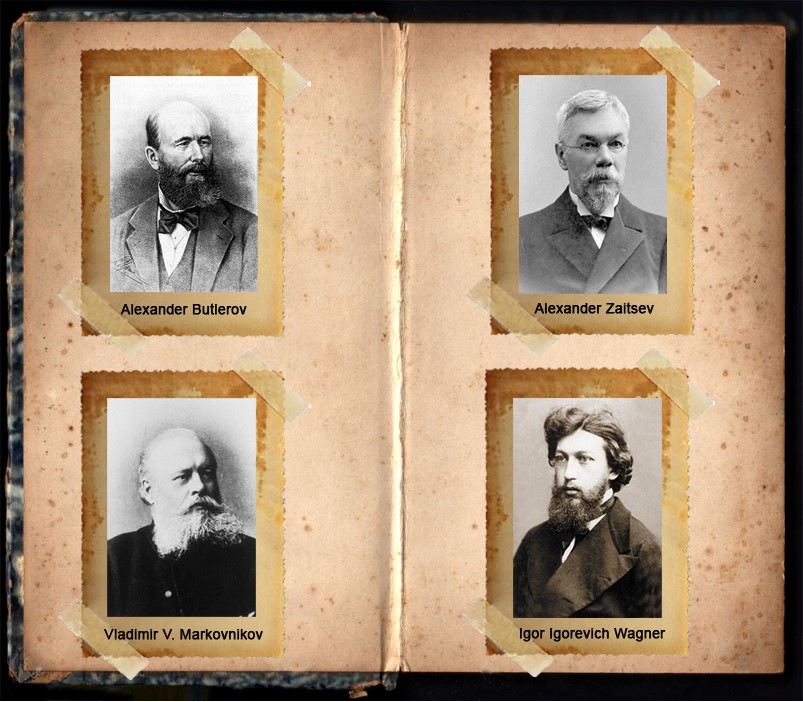
\includegraphics[width=12cm]{./pic/t4-1.jpg}
\end{figure}


\newpage
\mysection{第5题\  阿恩特-艾司特同系增碳反应}
阿恩特(Fritz Georg Arndt,1885.7.6--1969.12.8)是一位对土耳其的化学发展有着重要影响的德国化学家。在他的职业生涯中,他在土耳其伊斯坦布尔大学工作了二十余年。他和艾司特(Bernd Eistert)一同发现了阿恩特-艾司特合成法。这种合成法是一个可让羧酸碳链增长一个碳原子的反应,从而被称为同系增碳过程。在阿恩特-艾司特同系增碳反应中,关键的一步是利用沃尔夫重排(Wolff Rearrangement),在光照、加热或银(Ⅰ)盐催化下将重氮酮转化为烯酮。在亲核试剂如水、醇或胺的存在下,烯酮中间体会反应生成相应的羧酸、酯或酰胺。在本题中,我们会研究吲哚里西啶类生物碱的合成。

\textbf{\emph{(巨大的化学家帅照!)}}

根据以上描述,吲哚里西啶167B和去氢毒芹碱的合成易于通过β,γ-不饱和酯\textbf{B}实现。其关键的步骤(\textbf{A}→\textbf{B})是一步沃尔夫重排。化合物C含有内酰胺结构,且是一个包含六元环与饱和五元环稠合结构的双环杂环化合物,其中的一个桥头原子是氮原子。

\noindent\textbf{5.1.} 请画出\textbf{A-D}的机构(不需表示立体化学)。

\textbf{\emph{(大合成路线在此!)}}

在阿恩特-艾司特同系增碳反应中,α-重氮酮可以通过光引发的沃尔夫重排转化为α-羰基卡宾,并伴随着氮气的生成。这个中间体会经历一个1,2-烷基迁移从而给出烯酮产物。

\noindent\textbf{5.2.}
画出在第二步(\textbf{A}→\textbf{B})中α-羰基卡宾和烯酮中间体的结构。

以丙基溴化镁对化合物\textbf{C}进行加成,随后以AcOH/NaBH\textsubscript{4}处理,是吲哚里西啶167B全合成的最后一步。

\noindent\textbf{5.3.}
画出在第四步(\textbf{C}→\textbf{D})中中间体(\textbf{C\textsubscript{11}H\textsubscript{20}N\textsuperscript{+}})的结构。

\noindent\textbf{5.4.}
去氢毒芹碱的另一个合成方法描述如下。\textbf{\emph{画出}}化合物\textbf{E-J}的结构。

\textbf{\emph{(包含E-J未知物质的合成路线!)}}


\newpage
\mysection{第6题\  阿托伐醌}
阿托伐醌,亦作阿托喹酮或美普龙,是一种可用于治疗肺囊虫病以及疟疾、瘴气的药物。酮酯\textbf{1}和醛\textbf{2}是合成阿托伐醌的关键化合物。

\begin{figure}[h]
	\centering
	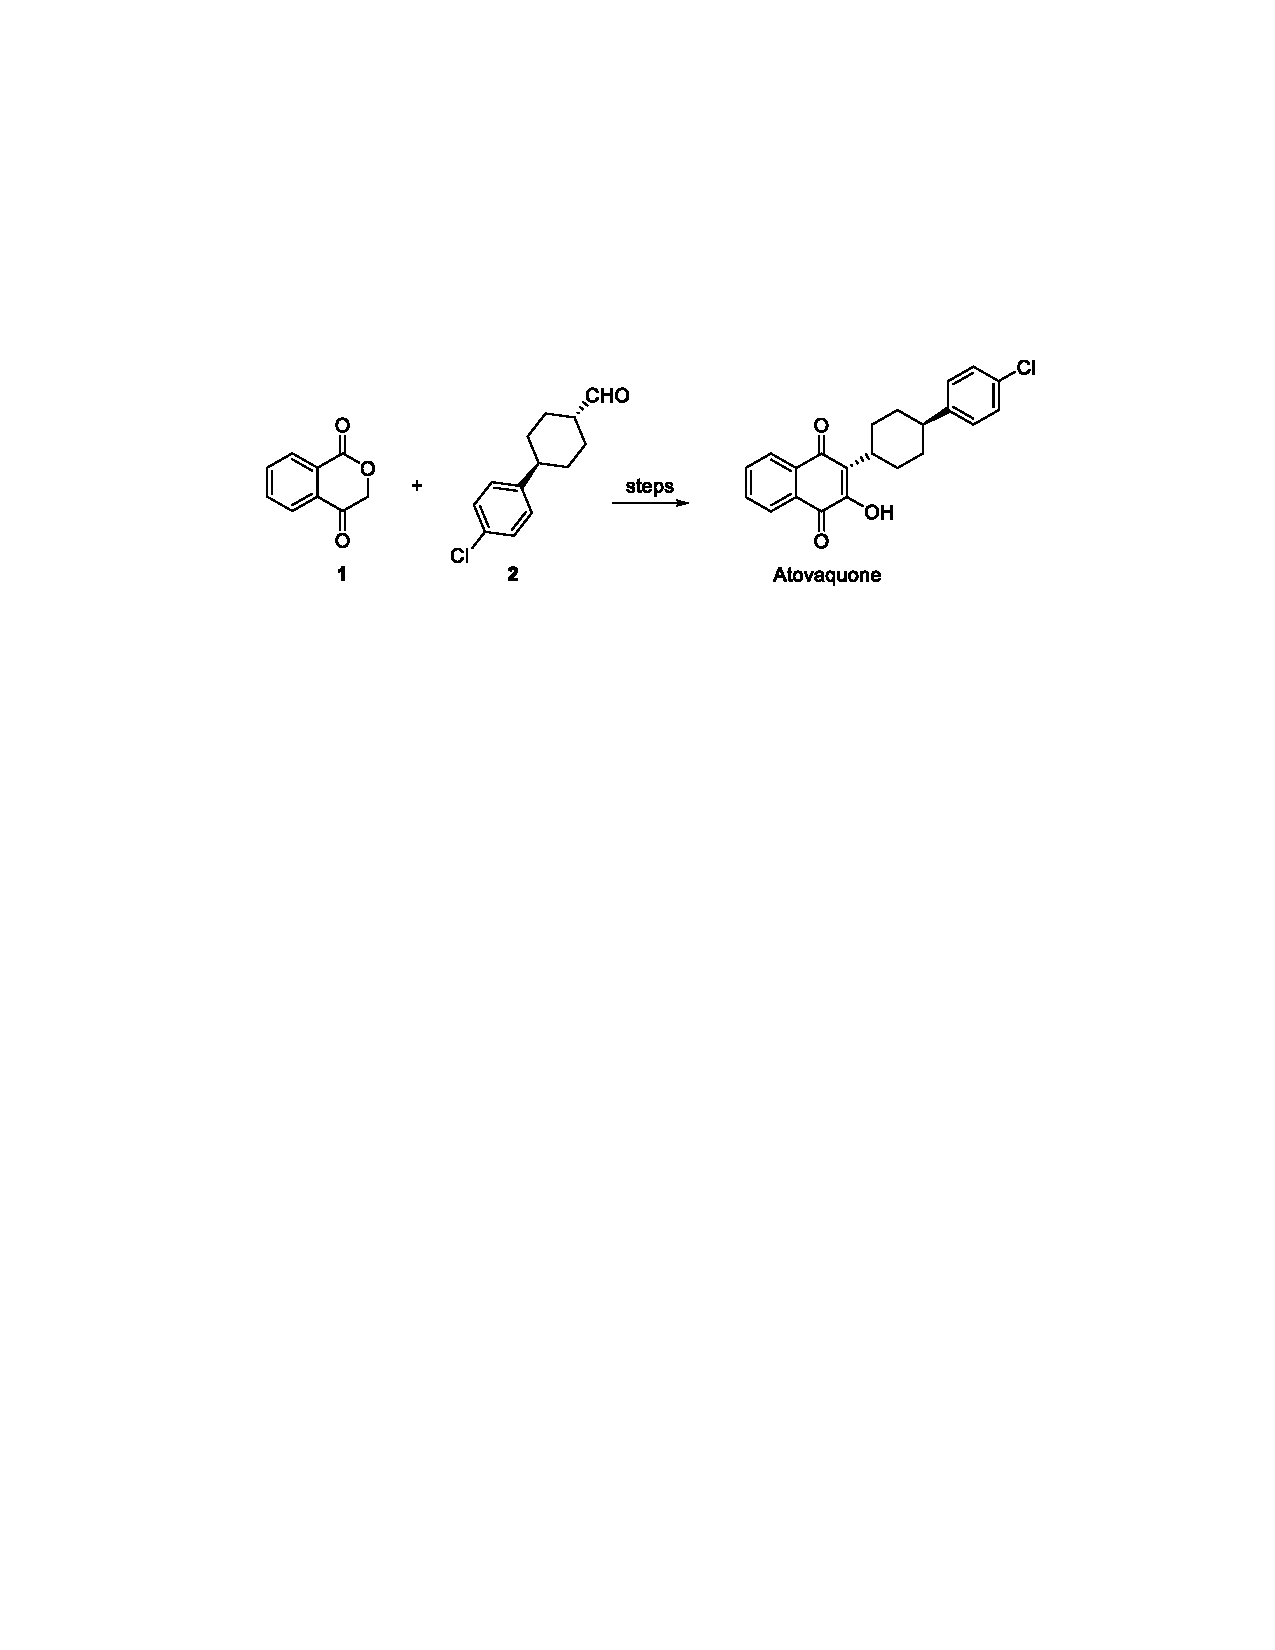
\includegraphics[width=14cm]{./pic/t6-1.pdf}
\end{figure}

关键化合物酮酯\textbf{1}的合成如下所示。将丙二酸在加热条件下加入邻苯二甲酸酐和三乙胺的混合物,在此过程中可观察到有气体逸出。以盐酸处理反应体系可经过有两个羧基的中间体\textbf{A}得到酸\textbf{3}。酸\textbf{3}可转化为分子式相同且包含半缩酮基团和酯基的中间体\textbf{B},随后脱水生成烯烃\textbf{C},再在酸性条件下溴化而生成\textbf{D}。二溴代物\textbf{D}在热的H\textsubscript{2}O/AcOH混合体系体系中溶剂解生成叔碳正离子中间体\textbf{E},随后\textbf{E}被水捕获生成中间体半缩酮\textbf{F},最后,中间体半缩酮\textbf{F}重排生成关键化合物\textbf{1}。

\noindent 注:方括号表示产物未进行分离和纯化而直接进行进一步反应。由\textbf{3}到\textbf{1}的转化是一个一锅煮反应,即不经对中间体的分离纯化而在同一个容器中一个接着一个发生的一系列反应。

\begin{figure}[h]
	\centering
	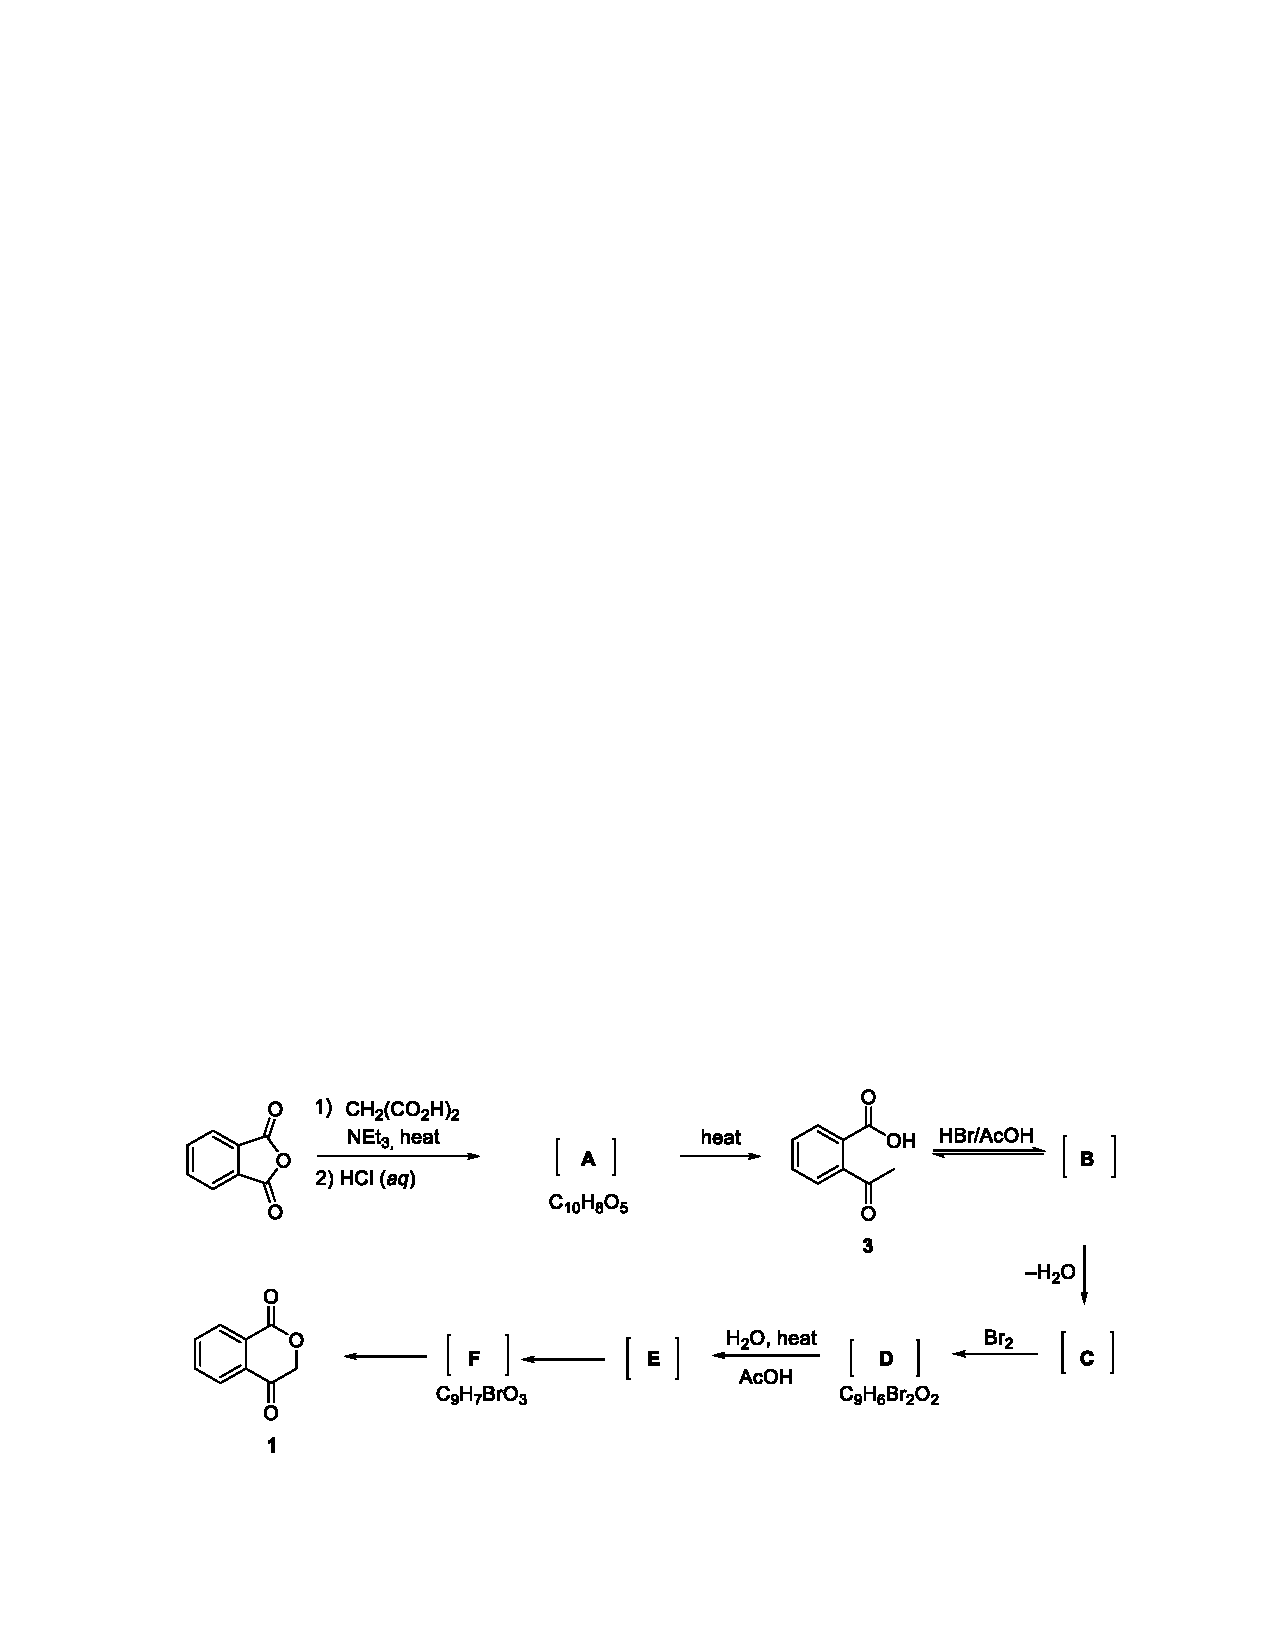
\includegraphics[width=16cm]{./pic/t6-2.pdf}
\end{figure}

中间体\textbf{B}和\textbf{C}的光谱数据:\textbf{B}:\textsuperscript{1}H NMR $\delta$ = 7.86-7.52 (4H), 4.13 (bs, 1H, 可与D\textsubscript{2}O交换), 1.97 (s, 3H). \textbf{C}:\textsuperscript{1}H NMR $δ$ = 7.92--7.58 (4H), 5.24 (m, 2H); \textsuperscript{13}C NMR δ = 166.8, 151.8, 139.0, 134.4, 130.4, 125.3, 125.1, 120.6, 91.3; MS m/z = 146.0

\noindent\textbf{6.1.} 画出在\textbf{1}的合成中中间体\textbf{A}-\textbf{F}的结构。

从环己烯开始可经由一系列关键步骤,包括傅-克酰基化反应、卤仿反应、还原反应和氧化反应合成关键化合物\textbf{2}。环己烯和乙酰氯进行傅-克酰基化反应生成氯代环己基甲基酮\textbf{J}。环己烯和乙酰氯的反应最初生成了碳正离子\textbf{G},随后连续进行了两次瓦格纳-梅尔外因重排先后生成分子式不变的碳正离子\textbf{H}和\textbf{I}。氯离子与碳正离子\textbf{I}反应生成了\textbf{J},\textbf{J}再与氯苯发生傅-克反应生成\textbf{K}。用次氯酸钠(NaOCl)与甲基酮\textbf{K}进行卤仿反应生成相应的酸\textbf{L},\textbf{L}再经由多步反应转化为醛\textbf{2}。

\noindent\textbf{6.2.} 画出分子式相同的碳正离子\textbf{G}-\textbf{I}的结构式。

\begin{figure}[h]
	\centering
	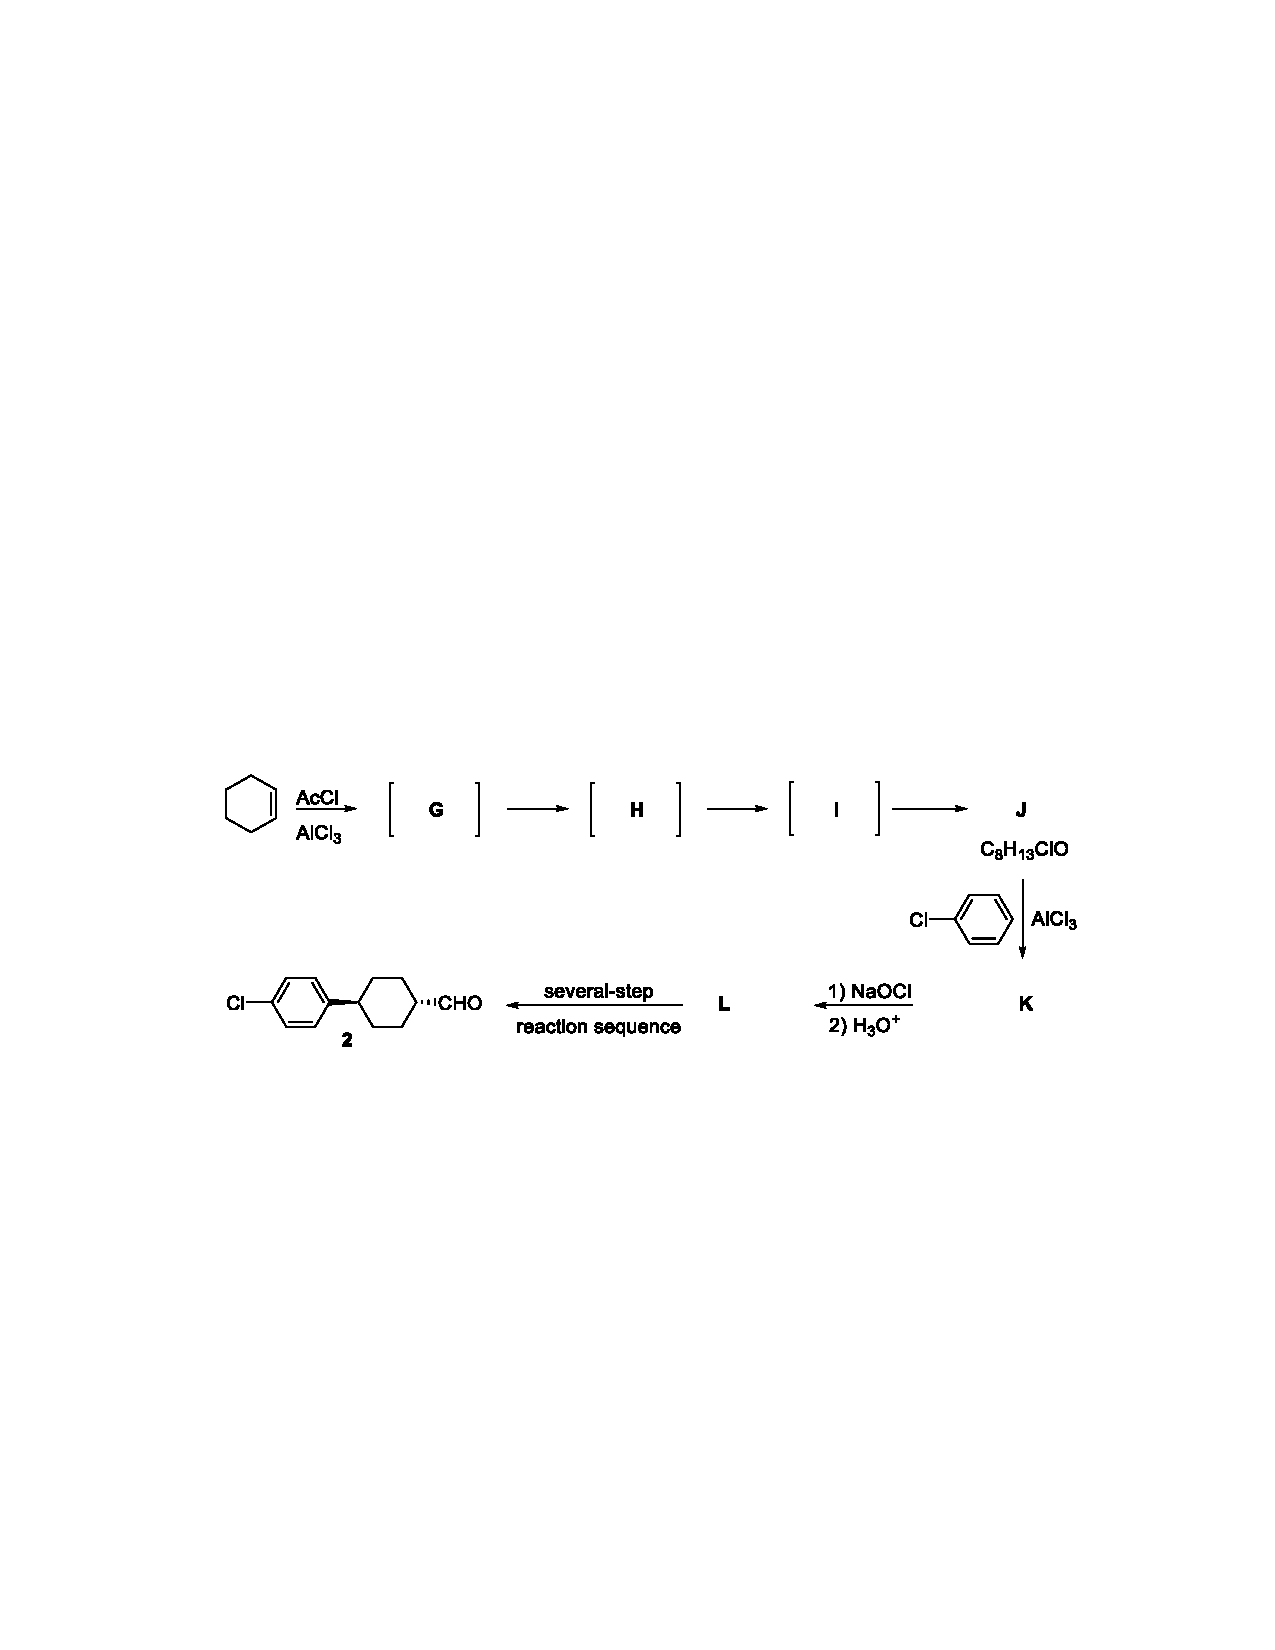
\includegraphics[width=15cm]{./pic/t6-3.pdf}
\end{figure}

\noindent\textbf{6.3.} 碳正离子\textbf{G}-\textbf{I}有手性吗?

\noindent\textbf{6.4.} 画出化合物\textbf{J}-\textbf{L}的结构。

\noindent\textbf{6.5.} 选出所有正确的选项。

\renewcommand{\labelitemi}{$\square$}
\begin{itemize}
	\item \textbf{L}有四个立体异构体。
	\item \textbf{L}是一个手性化合物。
	\item \textbf{L}是一个非手性化合物。
	\item \textbf{L}是一个内消旋化合物。
	\item \textbf{L}有两个立体异构体。
	\item \textbf{L}的立体异构体之间是非对映异构体。
	\item \textbf{L}的立体异构体之间是对映异构体。
\end{itemize}
\renewcommand{\labelitemi}{$\bullet$}

\noindent\textbf{6.6}下列化合物中哪个或哪些在卤仿反应中生成?

\renewcommand{\labelitemi}{$\square$}
\begin{itemize}
	\item CH\textsubscript{2}Cl\textsubscript{2}
	\item CH\textsubscript{3}Cl
	\item CHCl\textsubscript{3}
	\item CCl\textsubscript{4}
\end{itemize}
\renewcommand{\labelitemi}{$\bullet$}

\newpage\noindent\textbf{6.7}下列由化合物\textbf{L}生成醛\textbf{2}的反应条件有哪些是正确的?选出所有的正确答案。

\begin{figure}[h]
	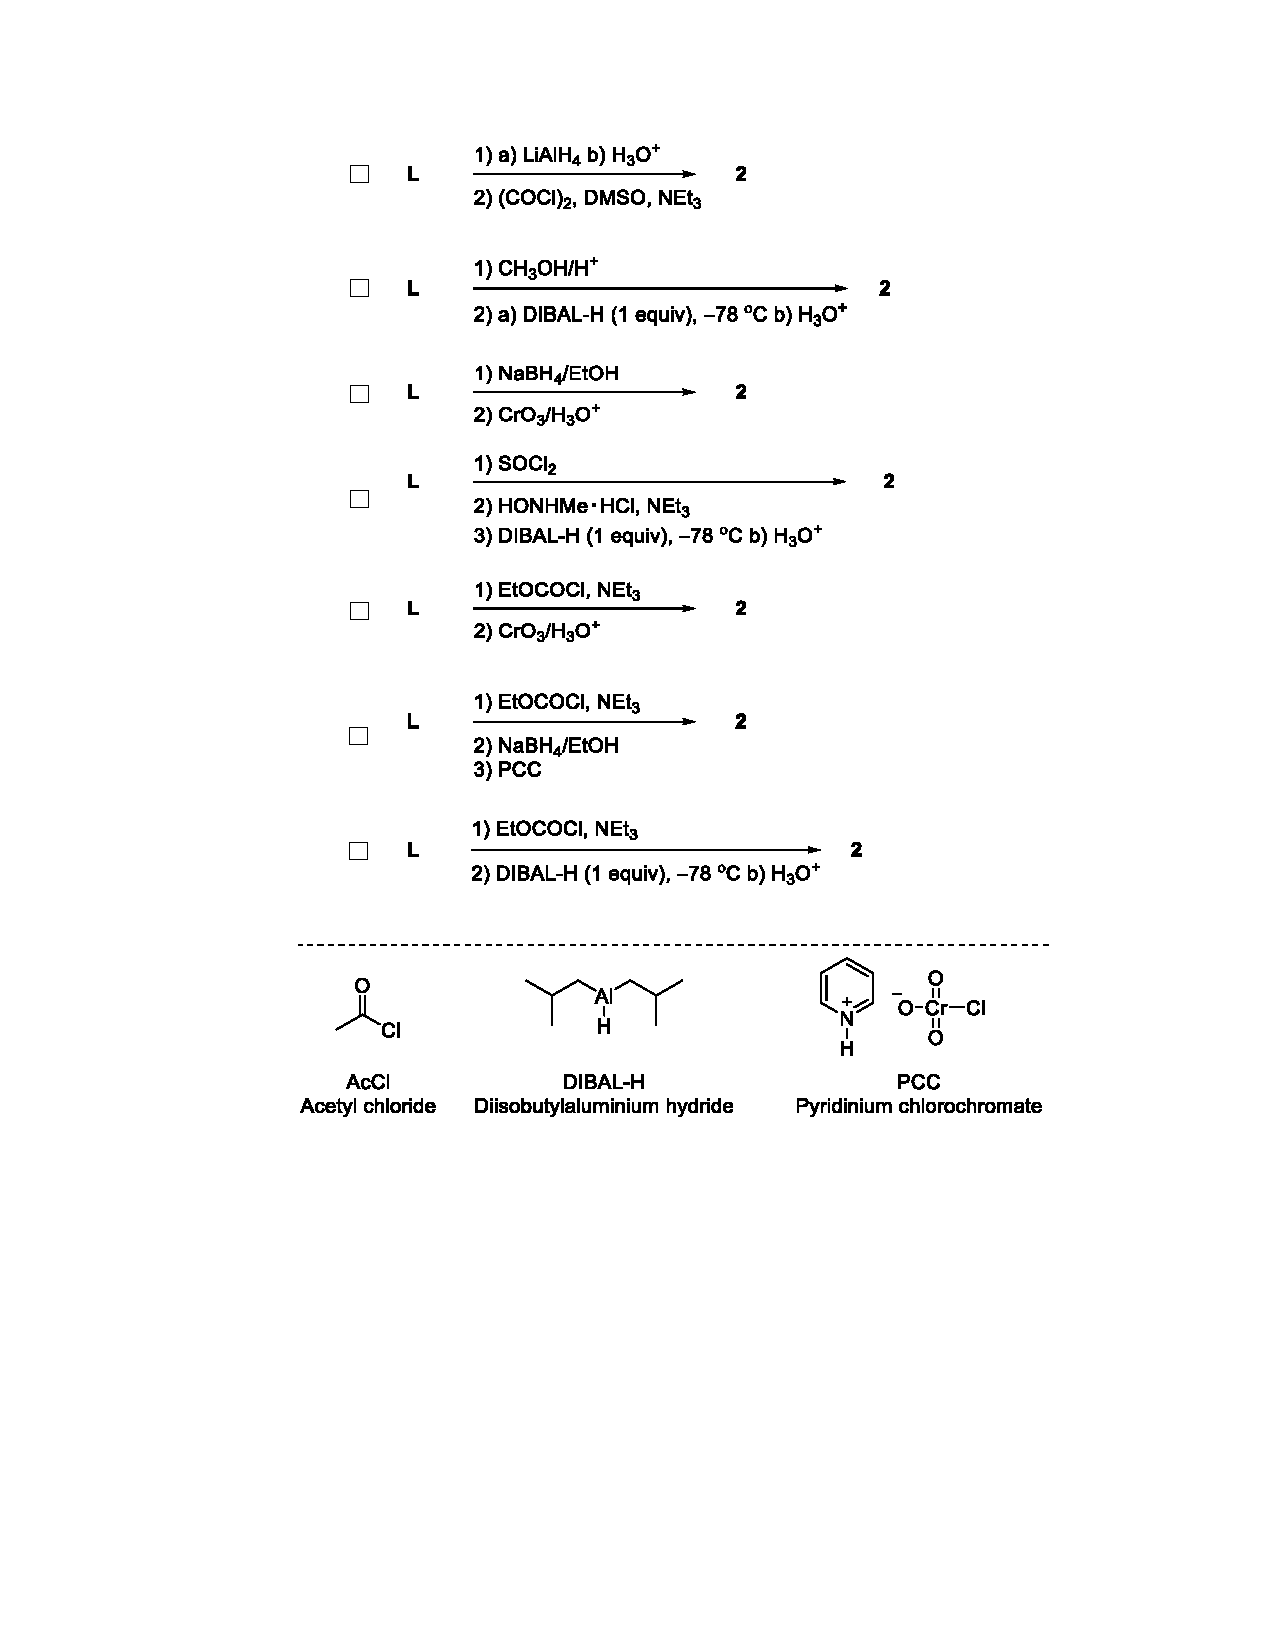
\includegraphics[width=14cm]{./pic/t6-4.pdf}
\end{figure}



\newpage
\mysection{第7题\  哪个是(±)-Trikentrin A}
虽然吲哚骨架在自然界中是普遍存在的,但是在苯环的任意位置上又加了个环的吲哚却并不常见。Trikentrins和结构相似的herbindoles代表了6,7-增环的吲哚或多烷基化的环戊烯基{[}g{]}吲哚天然产物。从蜘蛛海绵内分离出来的Trikentrin具有抗菌活性。下图展示了Trikentrin
A的可能结构。在此问题中,我们将找出以下结构中哪个是Trikentrin A。

\begin{figure}[h]
	\centering
	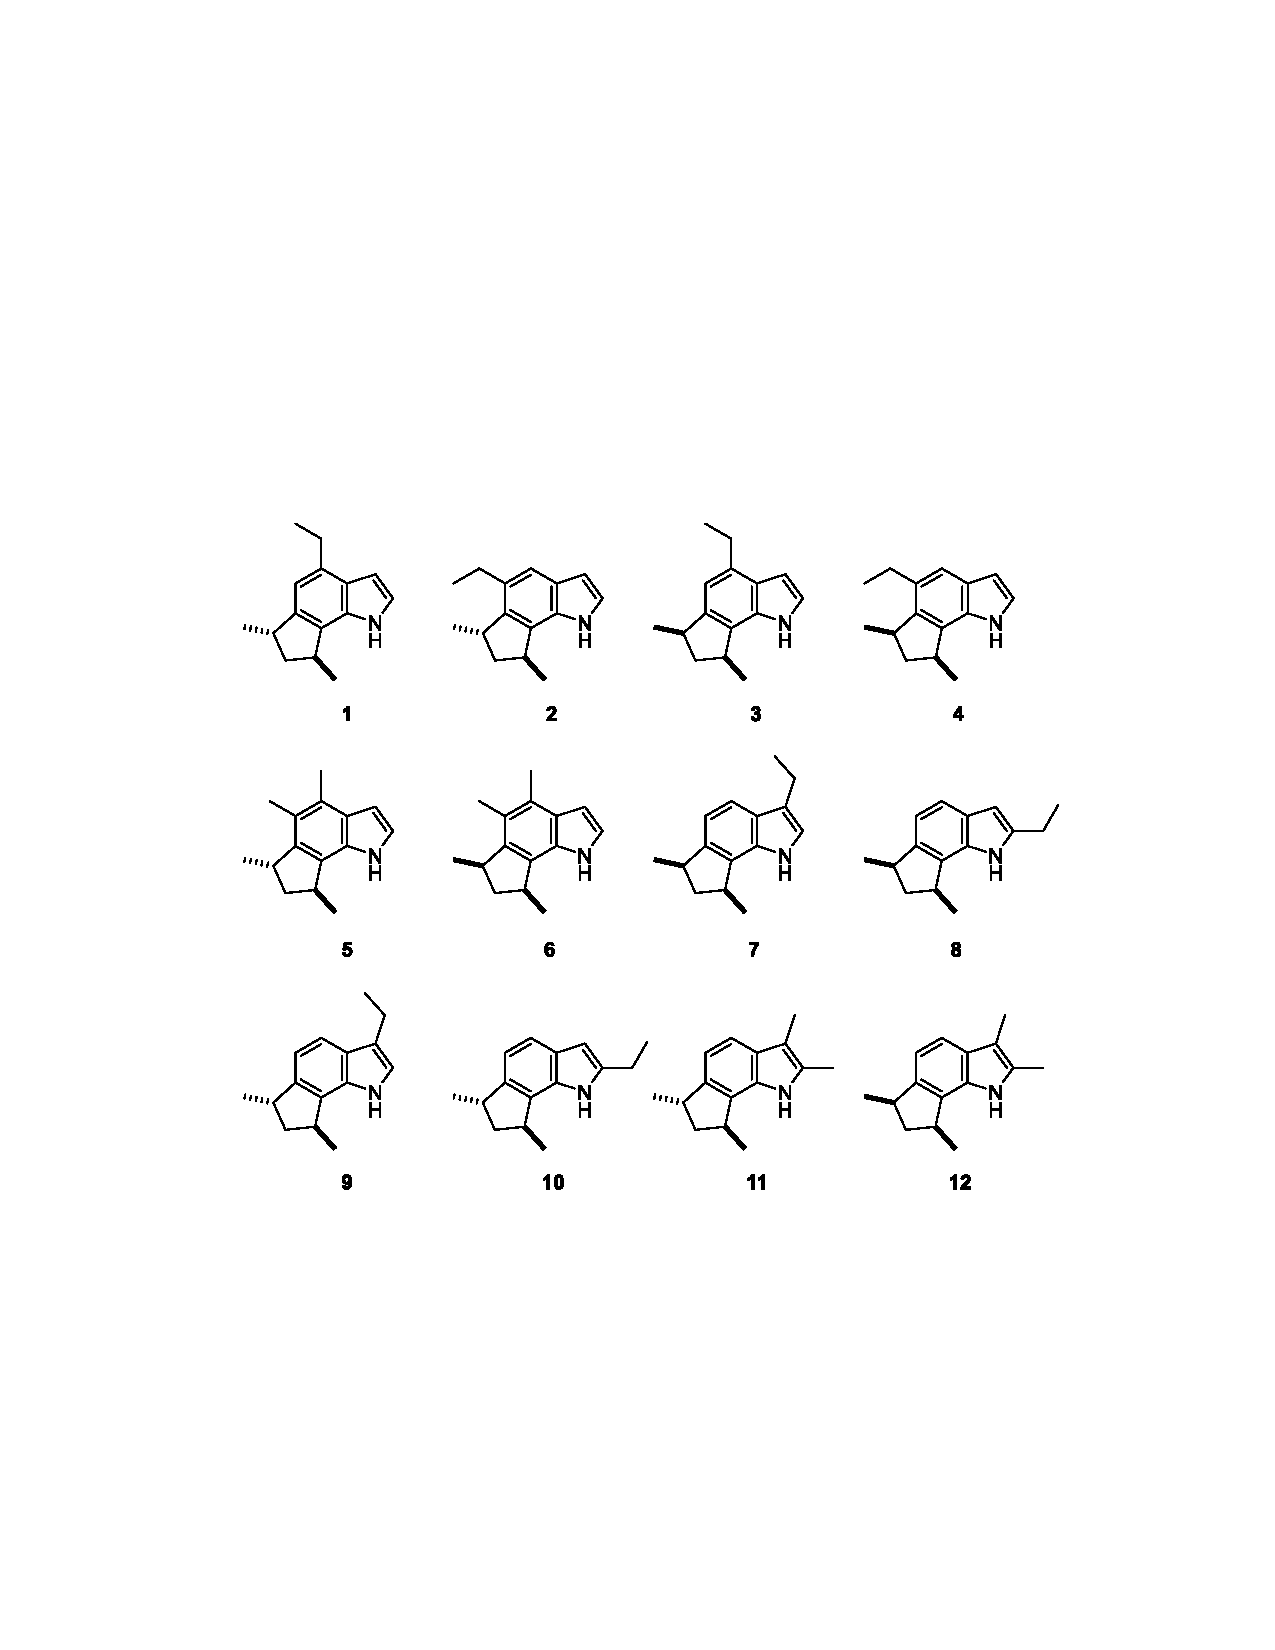
\includegraphics[width=14cm]{./pic/t7-1.pdf}
\end{figure}

合成Trikentrin
A的方法有几种:下面的两条路线包括基于芳炔的策略以及氢化乙烯基化的策略。试题7.1与7.2中的第一步是Bartoli吲哚合成法,即邻取代硝基芳香化合物与乙烯基格式试剂反应生成取代吲哚的反应。特别的,这也是合成7-取代吲哚的最有效的途径。

\begin{figure}[h]
	\centering
	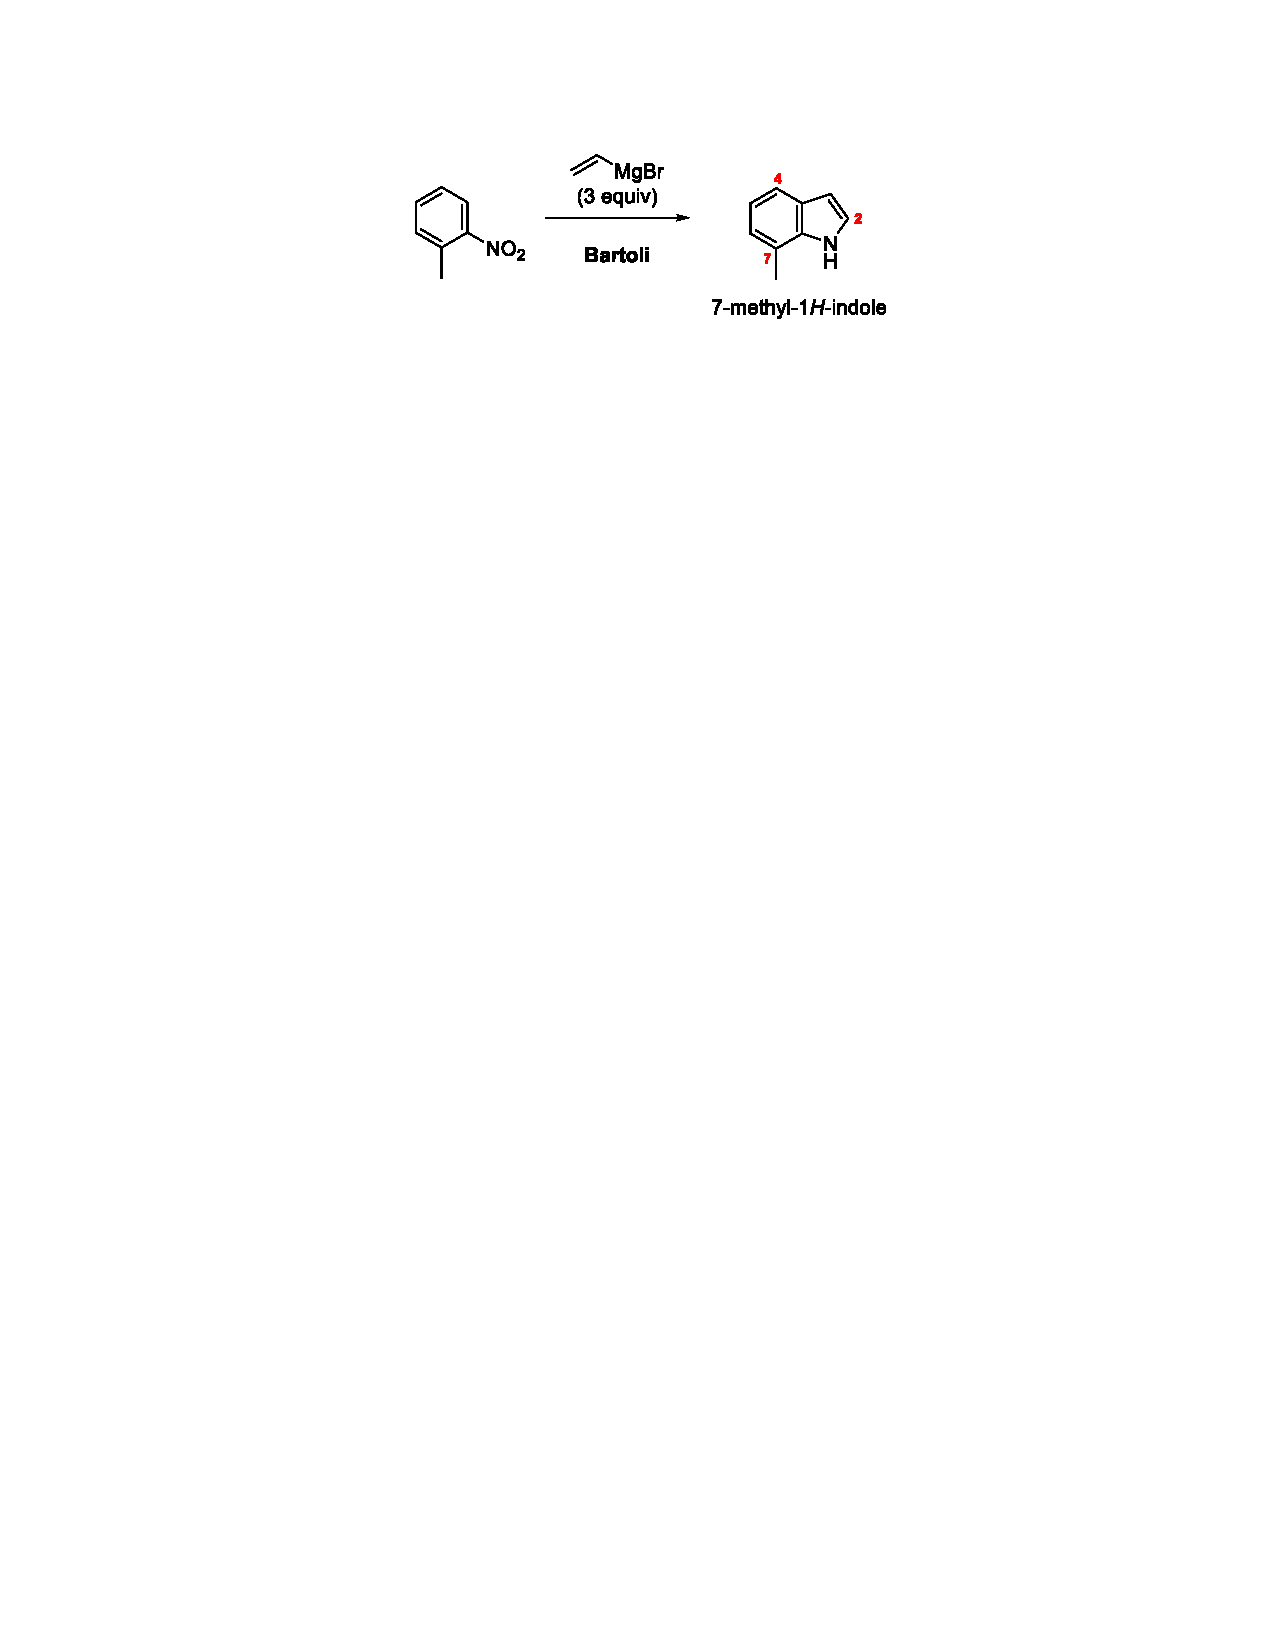
\includegraphics[width=9cm]{./pic/t7-2.pdf}
\end{figure}

\noindent(±)-Trikentrin A\textbf{:} \textsuperscript{1}H NMR
(CDCl\textsubscript{3}): $\delta$ 8.08 (bs, NH, 1H), 7.15−6.59 (3H), 3.44 (dt, \emph{J} = 8.8, 7.5 Hz, 1H), 3.22 (dt, \emph{J} = 8.8, 7.5 Hz, 1H), 2.94 (dq, \emph{J} = 15.0, 7.5 Hz, 1H), 2.93 (dq, \emph{J} = 15.0, 7.5 Hz, 1H), 2.60 (dt, \emph{J} = 12.3, 7.5 Hz, 1H), 1.50 (d, \emph{J} = 6.8 Hz, 3H), 1.37 (d, \emph{J} = 7.0 Hz, 3H), 1.36 (t, \emph{J} = 7.5 Hz, 3H), 1.32 (dt, \emph{J} = 12.3, 8.8 Hz, 1H); \textsuperscript{13}C NMR (CDCl\textsubscript{3}): $\delta$ 143.4−101.6 (8 signals), 44.8−15.1 (7 signals).

\newpage\noindent\textbf{基于芳炔的策略}

\begin{figure}[h]
	\centering
	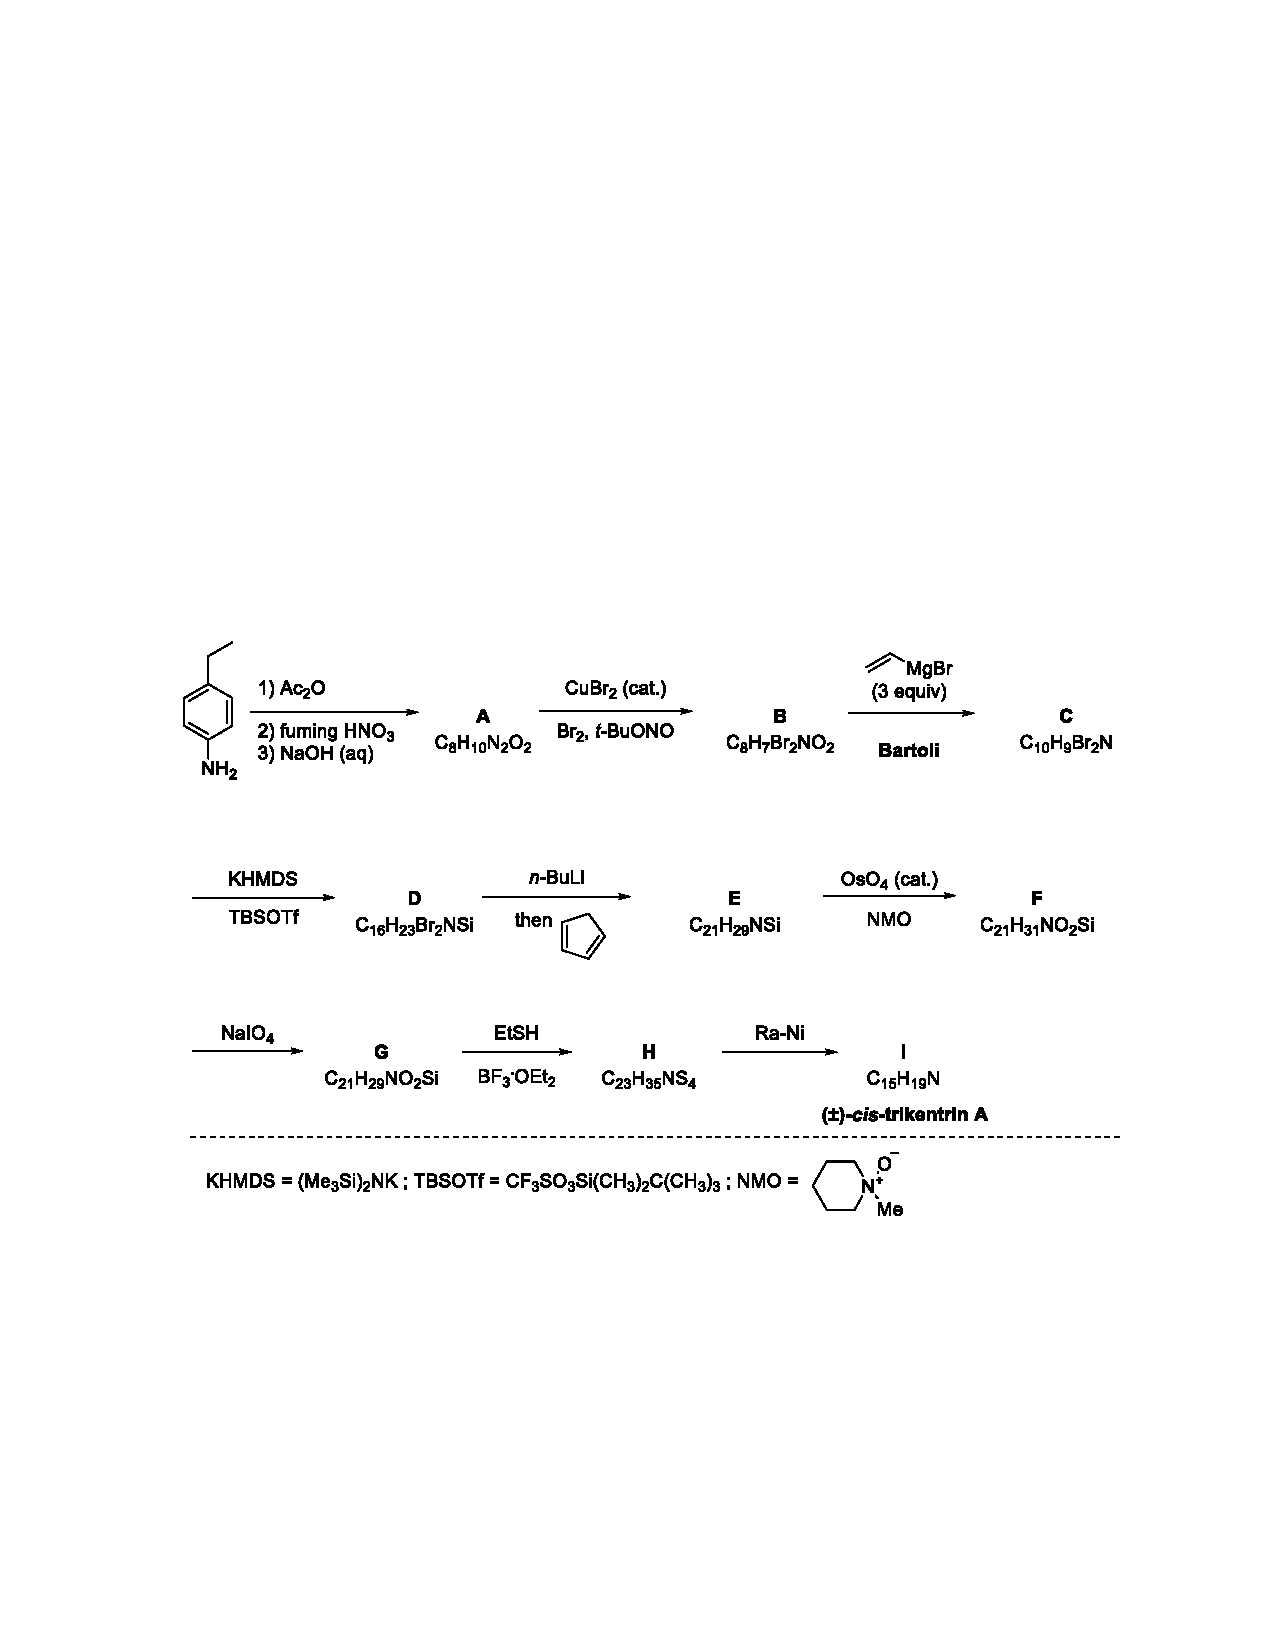
\includegraphics[width=16cm]{./pic/t7-3.pdf}
\end{figure}

\noindent\textbf{7.1.} 画出\textbf{A}-\textbf{I}的结构。

\noindent\textbf{7.2.} 画出步骤\textbf{D}-\textbf{E}中芳炔中间体的结构。

\noindent\textbf{氢化乙烯基化策略}

\begin{figure}[h!]
	\centering
	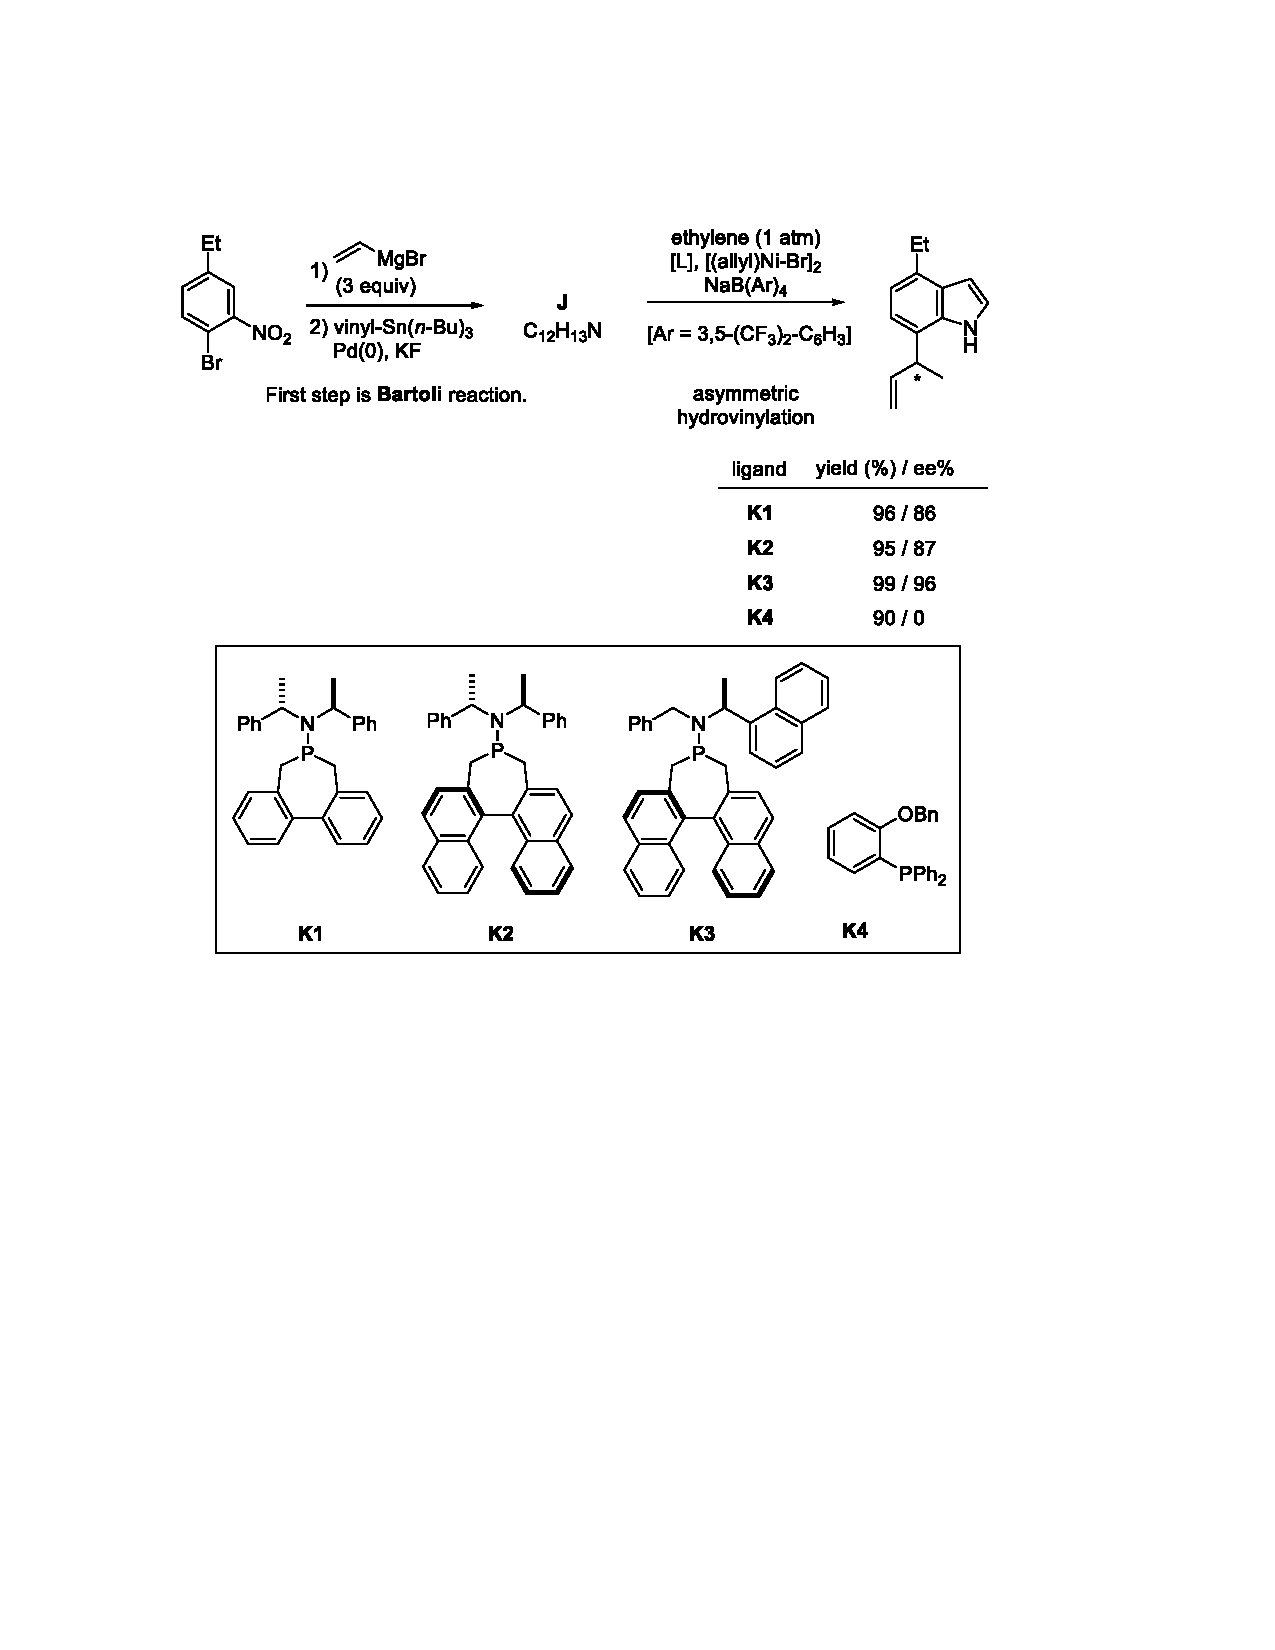
\includegraphics[width=14cm]{./pic/t7-4.pdf}
\end{figure}

\noindent\textbf{7.3.}
从溴代硝基苯到对应的7-乙烯基吲哚\textbf{J}的转化包括了Bartoli吲哚合成法及随后使用乙烯基锡的乙烯基化。画出\textbf{J}的结构。

第二步是Ni(II)催化的不对称氢化乙烯基化反应。该反应的配体\textbf{K1}-\textbf{K4}已在上图给出。

\noindent 注:ee为对映体过量,ee\%=占多数的对映体百分含量-占少数的对映体百分含量

\noindent\textbf{7.4.} 判断以下陈述:

\renewcommand{\labelitemi}{$\square$}
\begin{itemize}
\item 配体\textbf{3}给出了最好的对映体选择性
\item 配体\textbf{4}给出了外消旋体
\item 以上四个配体都是具有手性的
\item 以上四个配体都给出了很高的产率(\textgreater{}95\%)
\end{itemize}
\renewcommand{\labelitemi}{$\bullet$}

\noindent\textbf{7.5.} 对于氢化乙烯基化一步,判断以下陈述:

\renewcommand{\labelitemi}{$\square$}
\begin{itemize}
\item 烯丙基溴化镍是乙烯基的来源。
\item 在此烯丙基镍配合物中,镍的氧化态为+2。
\item 在此烯丙基镍配合物中,镍的外层电子数为18。
\item 此镍配合物具有平面四方的立体构型。
\end{itemize}
\renewcommand{\labelitemi}{$\bullet$}

\begin{figure}[h!]
	\centering
	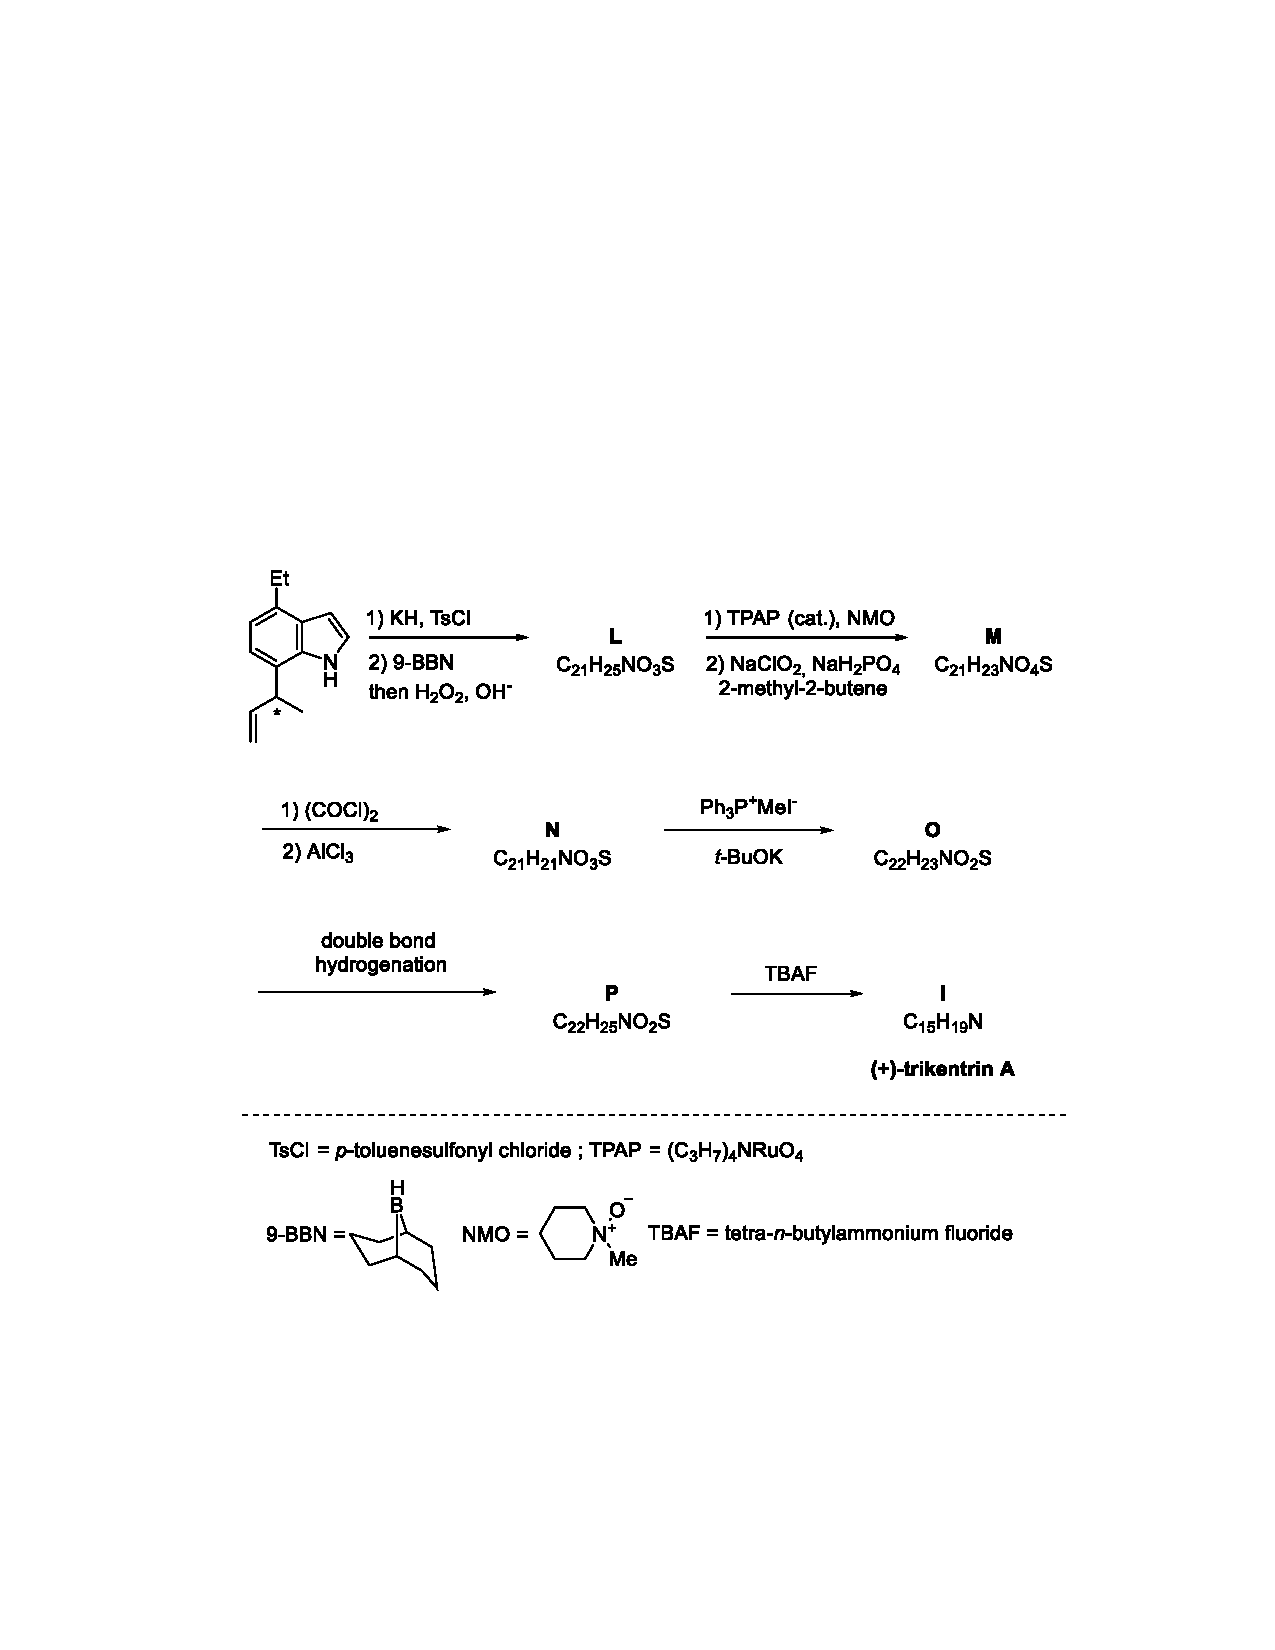
\includegraphics[width=14cm]{./pic/t7-5.pdf}
\end{figure}

\noindent\textbf{7.6.}
画出\textbf{L-P}的结构。氢化乙烯基化的产物之绝对构型为S。提示:在化合物\textbf{M}的\textsuperscript{13}C
NMR谱中,有一个峰在$\delta$ = 178.33 ppm处被观测到。


\textbf{\\
}


\newpage
\mysection{第8题\  1,2,3-三苯基丙-1,3-二醇的立体异构体}
\begin{figure}[h]
	\centering
	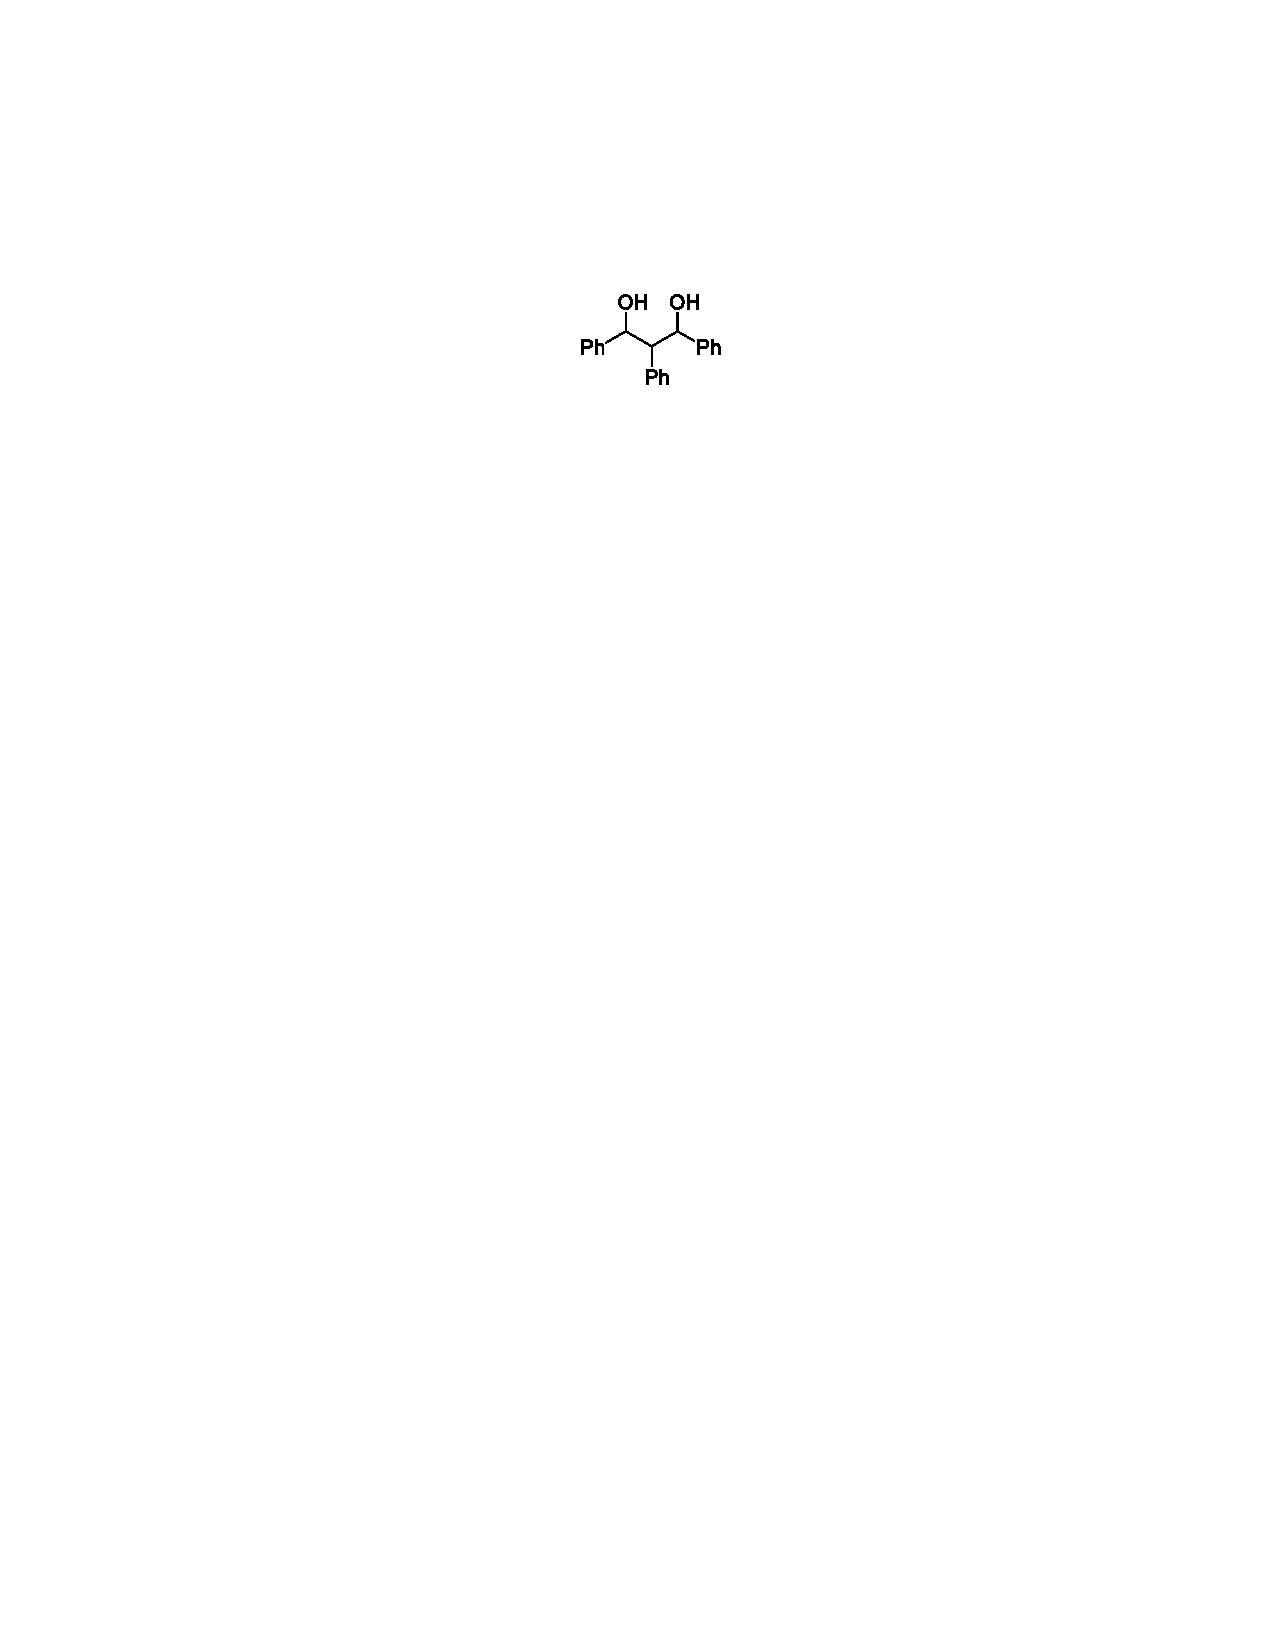
\includegraphics[width=5cm]{./pic/t8-1.pdf}
\end{figure}

\noindent\textbf{8.1.} 画出1,2,3-三苯基丙-1,3-二醇的所有立体异构体。

\noindent\textbf{8.2.} 列出其中所有的非手性化合物。

\noindent\textbf{8.3.} 列出其中所有的手性化合物。

\noindent\textbf{8.4.} 下列哪一些性质或者方法可以用来区分问题8.3中的手性化合物?选择所有正确的观点。

\renewcommand{\labelitemi}{$\square$}
\begin{itemize}
\item 沸点
\item 紫外光谱
\item 折射率
\item 熔点
\item 旋光度
\item 偶极矩
\item 非手性环境中的核磁共振
\item 红外光谱
\end{itemize}
\renewcommand{\labelitemi}{$\bullet$}


\newpage
\mysection{第9题\  核磁共振,对称性与结构分析}
\paragraph{卤代萘:应用广泛的关键化合物}

除了苯之外,萘也是广为人知的芳香烃之一。因此,萘\textbf{1}的化学被广为研究而且许多萘的衍生物已经被合成了出来。其中,它的卤代物是许多转化中的关键。为此,几乎所有的卤代萘在文献中都有出现。对称化合物的\textsuperscript{1}H与\textsuperscript{13}C
NMR谱都很有特点,这就使得研究者排除可能的不对称化合物来分析对称的化合物。下面让我们来考虑四溴代萘\textbf{2}的异构体们。

\begin{figure}[h]
	\centering
	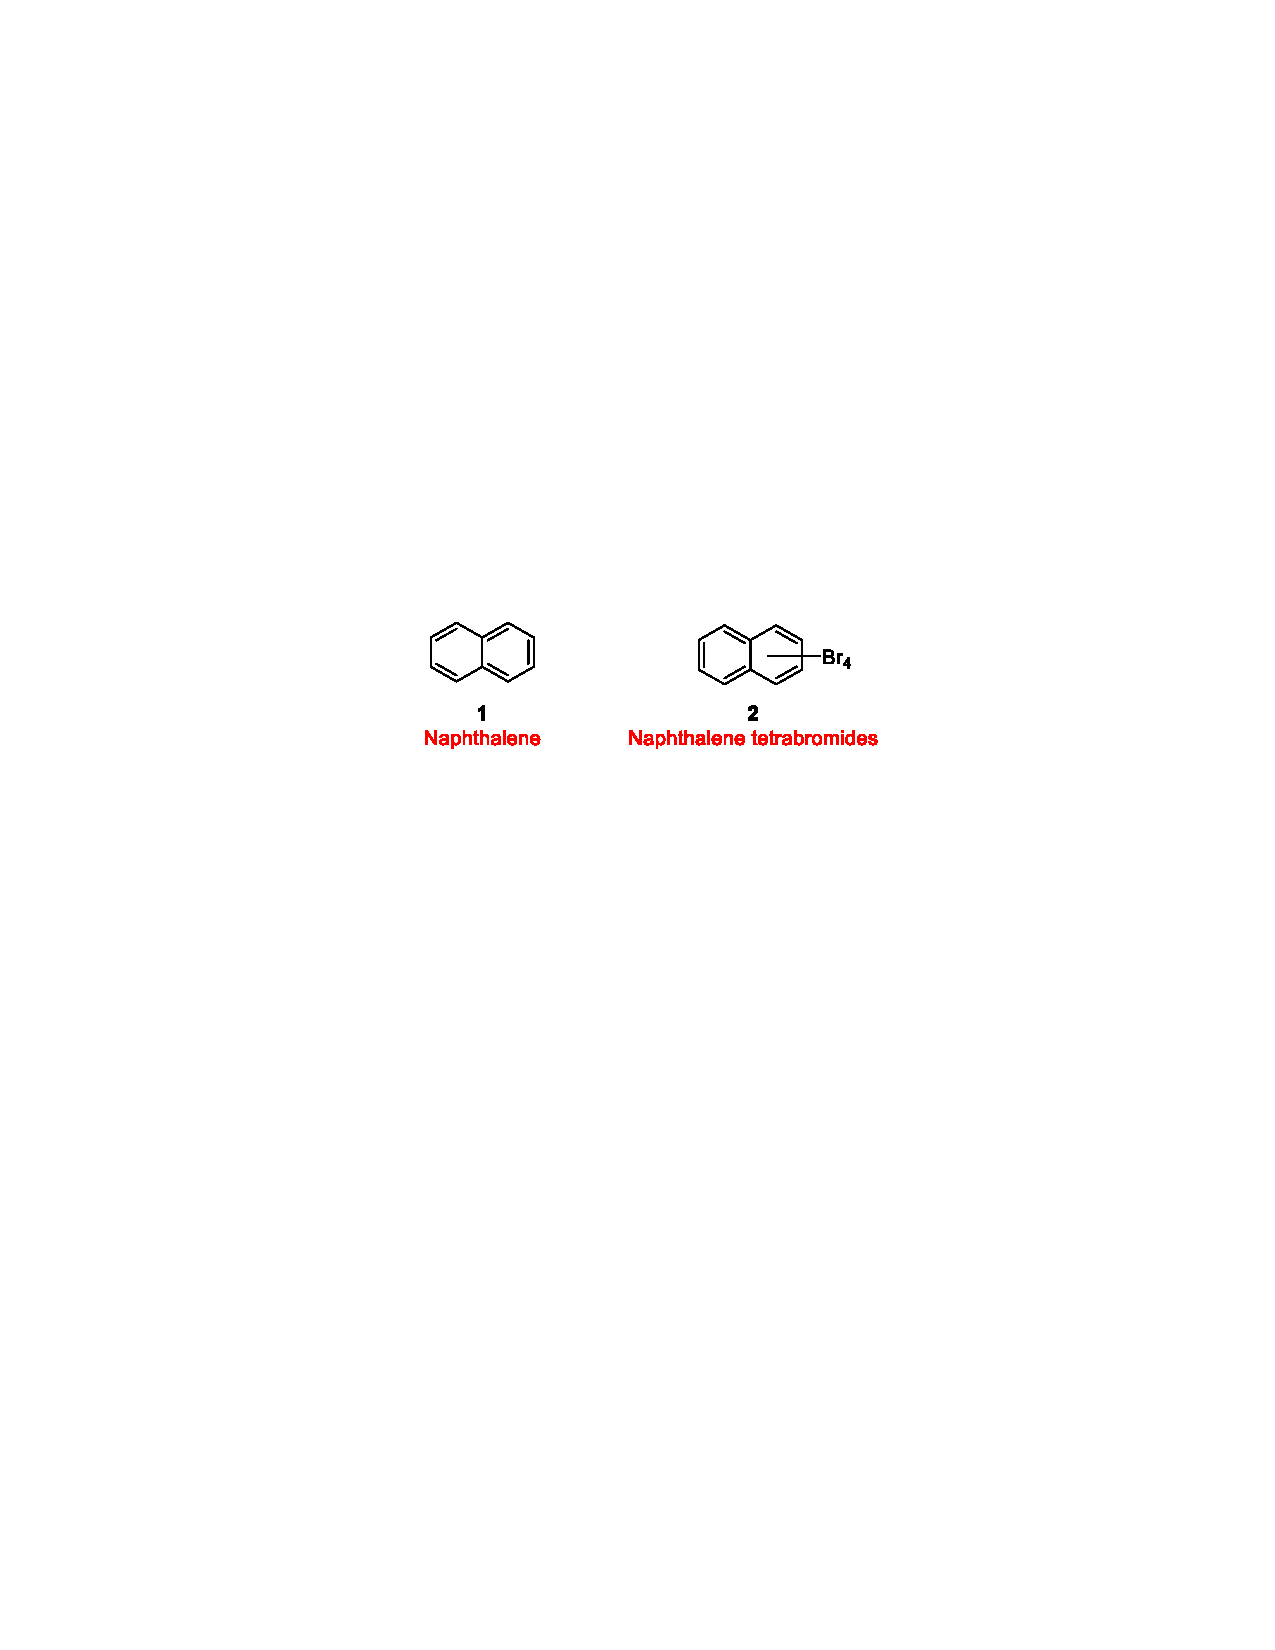
\includegraphics[width=9cm]{./pic/t9-1.pdf}
\end{figure}


\noindent\textbf{9.1.} 画出所有\textsuperscript{13}C
NMR具有三个信号且\textsuperscript{1}H NMR仅含一个信号的四溴代萘异构体。

\noindent\textbf{9.2.} 画出所有\textsuperscript{13}C
NMR具有五个信号的四溴代萘异构体。

\noindent\textbf{9.3.} 画出所有\textsuperscript{13}C
NMR具有六个信号且\textsuperscript{1}H NMR含一个二重峰(\emph{J} = 8-9
Hz)的四溴代萘异构体。

\noindent\textbf{9.4.} 画出所有\textsuperscript{13}C
NMR具有六个信号且\textsuperscript{1}H NMR含一个二重峰(\emph{J} = 1.5-2.0
Hz)的四溴代萘异构体。

\paragraph{动态核磁共振:在NMR中互变异构体的快速转化}

瞬烯\textbf{3}非常容易发生简并的Cope重排。不考虑对映体,瞬烯重排产生的可分辨的互变异构体共有10!/3 = 1,209,600个。这样的重排使得所有的碳原子和氢原子在核磁共振的时间尺度下均是等价的。在足够高的温度下,核磁共振碳谱与氢谱均只显示一个宽峰。然而,在−60 °C,此时Cope重排不可发生,烯基氢跟烷基氢就可以分辨了。

\begin{figure}[h]
	\centering
	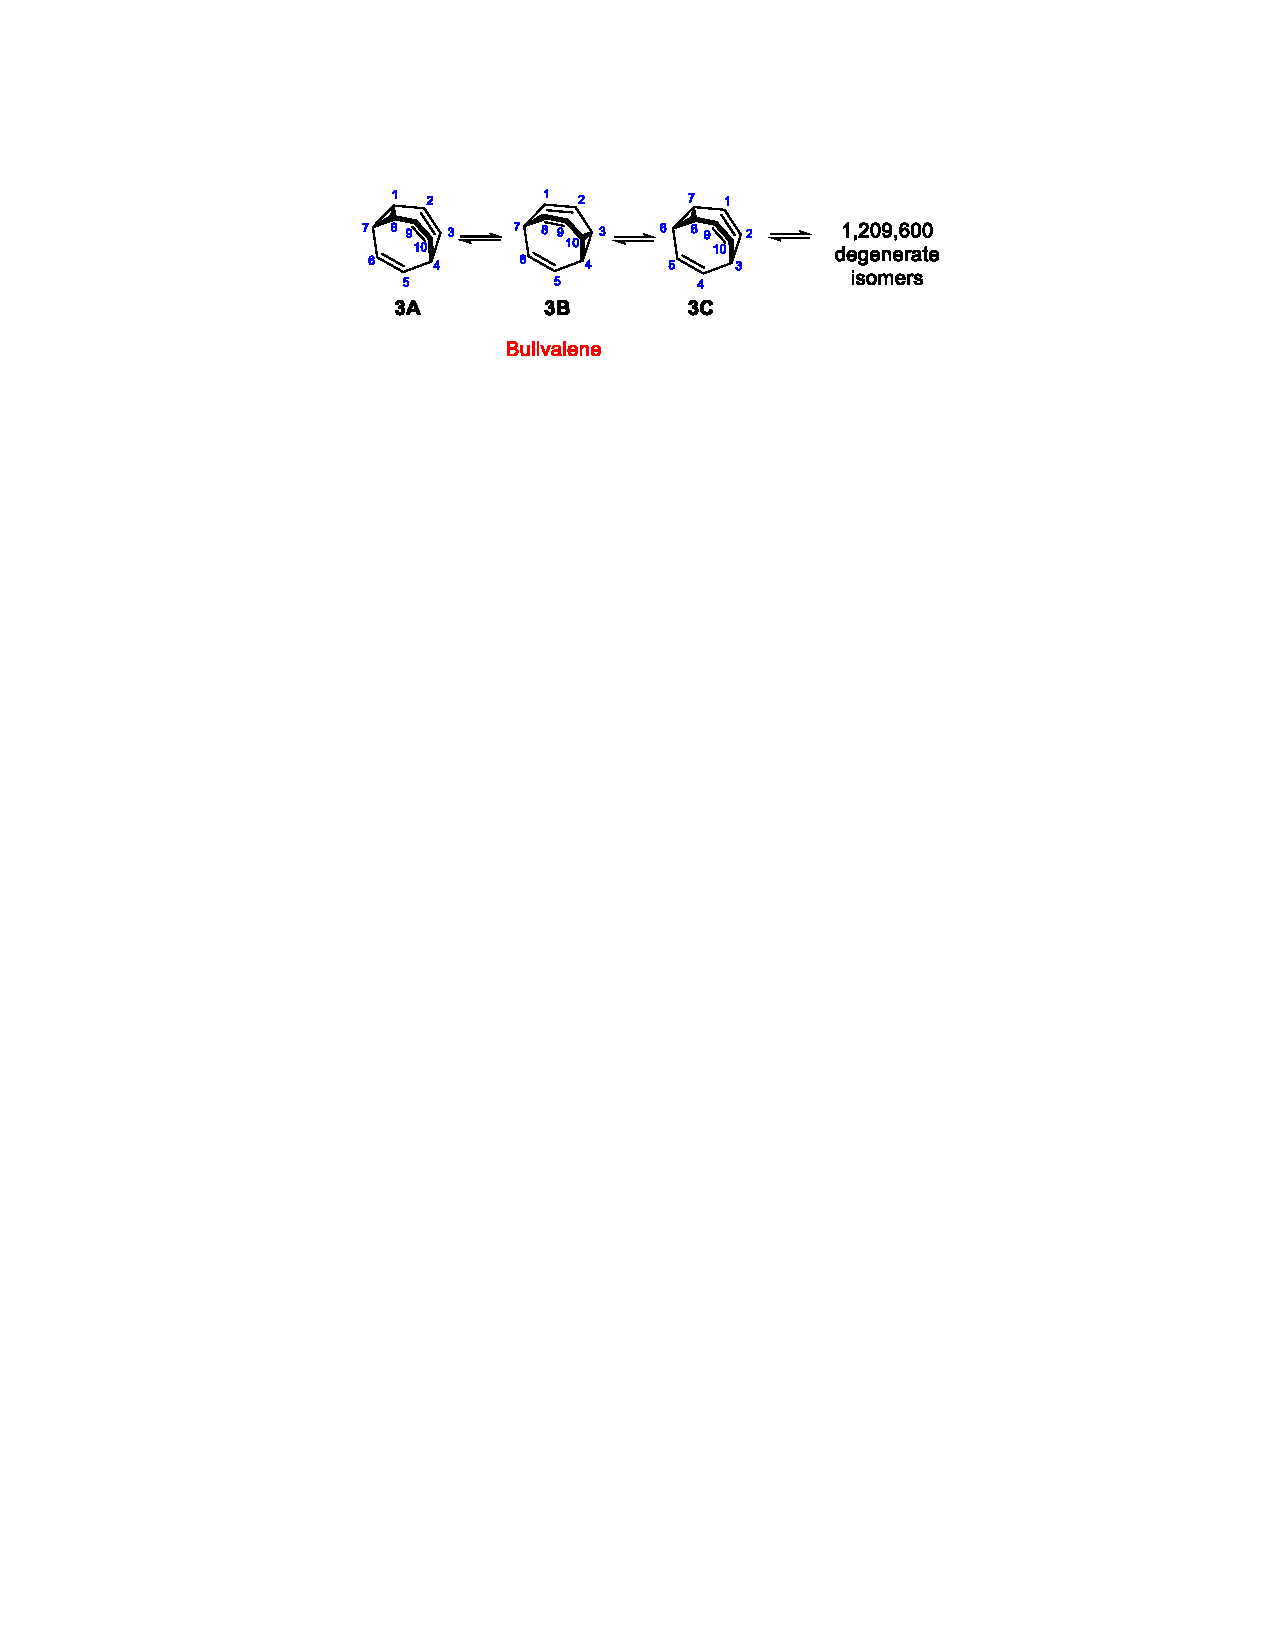
\includegraphics[width=10cm]{./pic/t9-2.pdf}
\end{figure}

\noindent\textbf{9.5.} 低温时,不考虑任何的Cope重排,\textsuperscript{13}C
NMR谱中应有多少个峰?用\textbf{a},\textbf{b},\textbf{c}\ldots{}在分子结构中标记相同的碳原子。

\noindent\textbf{9.6.}
某些分子因互变异构带来的形式上的对称性而给出更清晰的核磁共振谱。根据此信息,您觉得以下化合物的\textsuperscript{13}C
NMR各有多少个峰呢?

\begin{figure}[h]
	\centering
	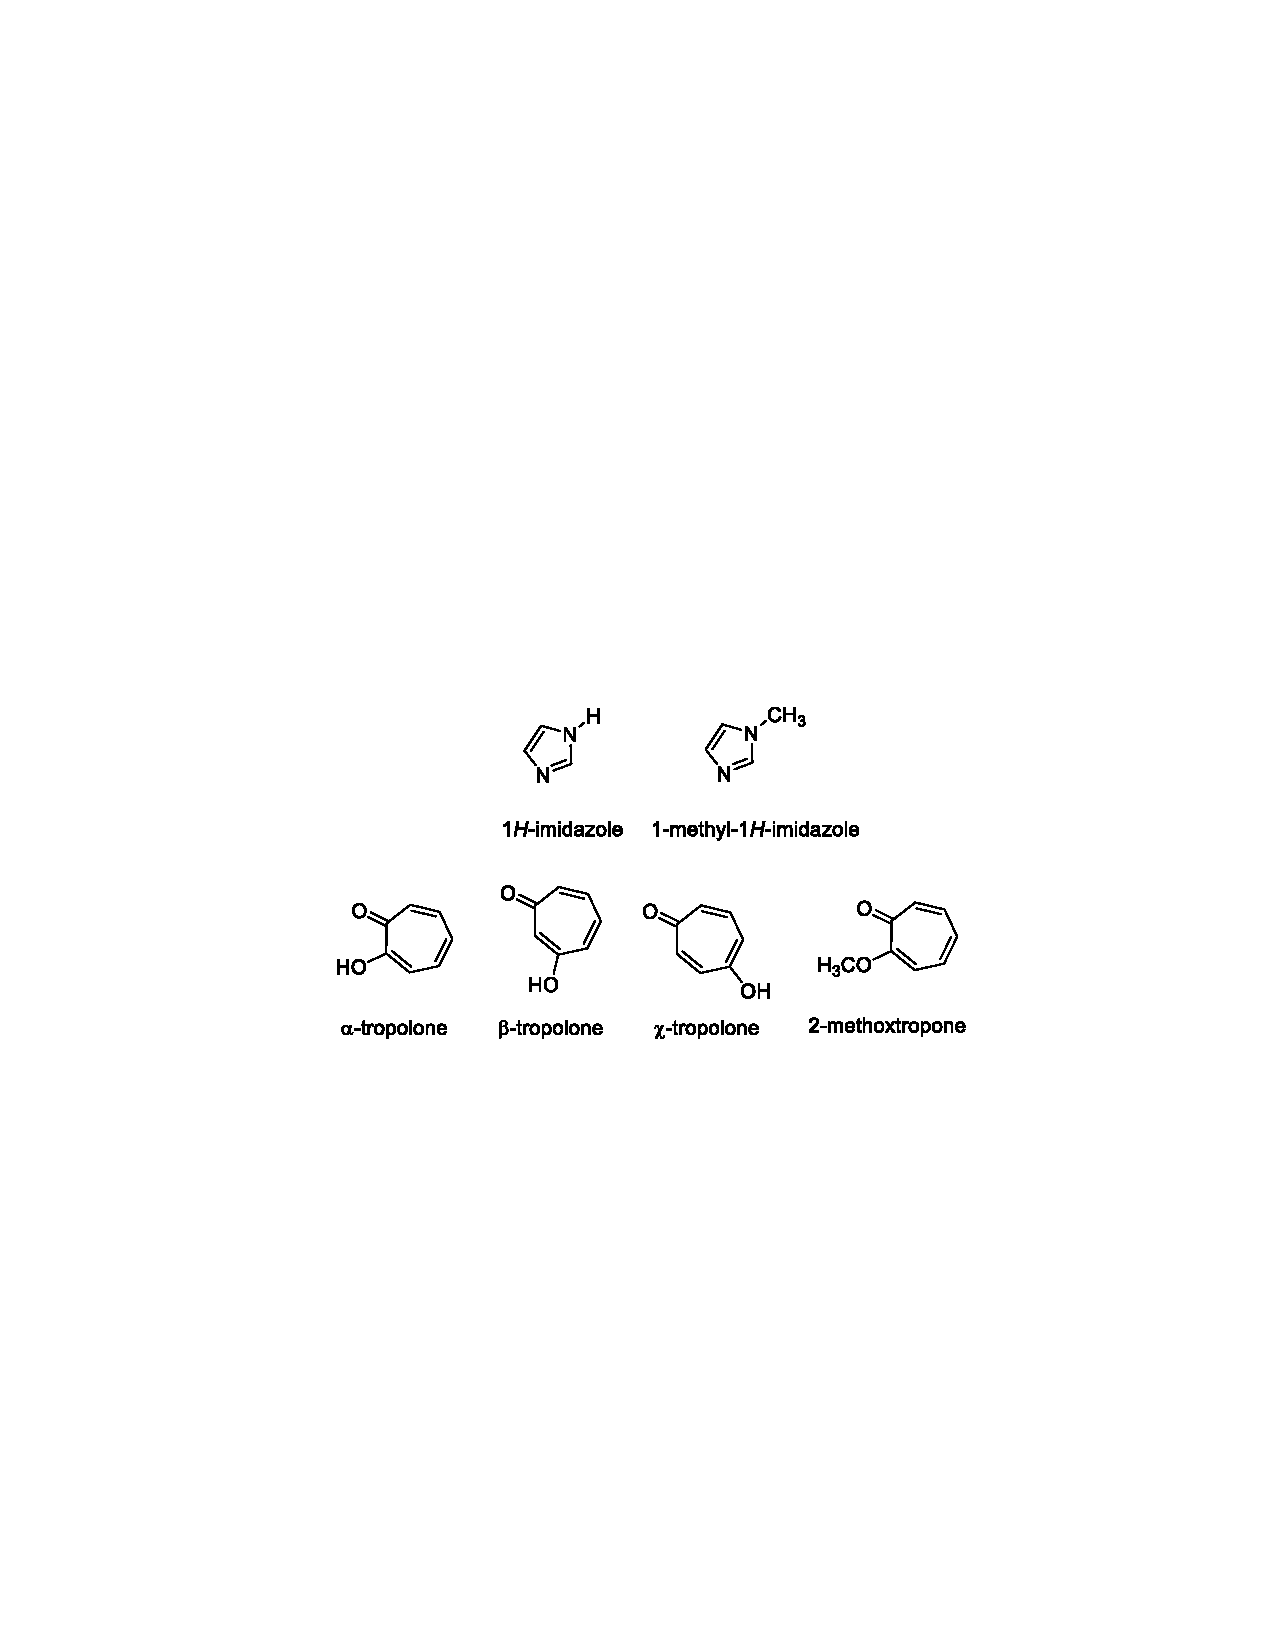
\includegraphics[width=11cm]{./pic/t9-3.pdf}
\end{figure}

\newpage\noindent\textbf{9.7.}
在文献中表明,环庚三烯酚酮衍生物\textbf{4}的\textsuperscript{13}C NMR谱比预料中少了几个峰。

画出合理的共振结构和/或转化来体现这种对称性。您觉得以下化合物的\textsuperscript{13}C NMR各有多少个峰呢?

\begin{figure}[h]
	\centering
	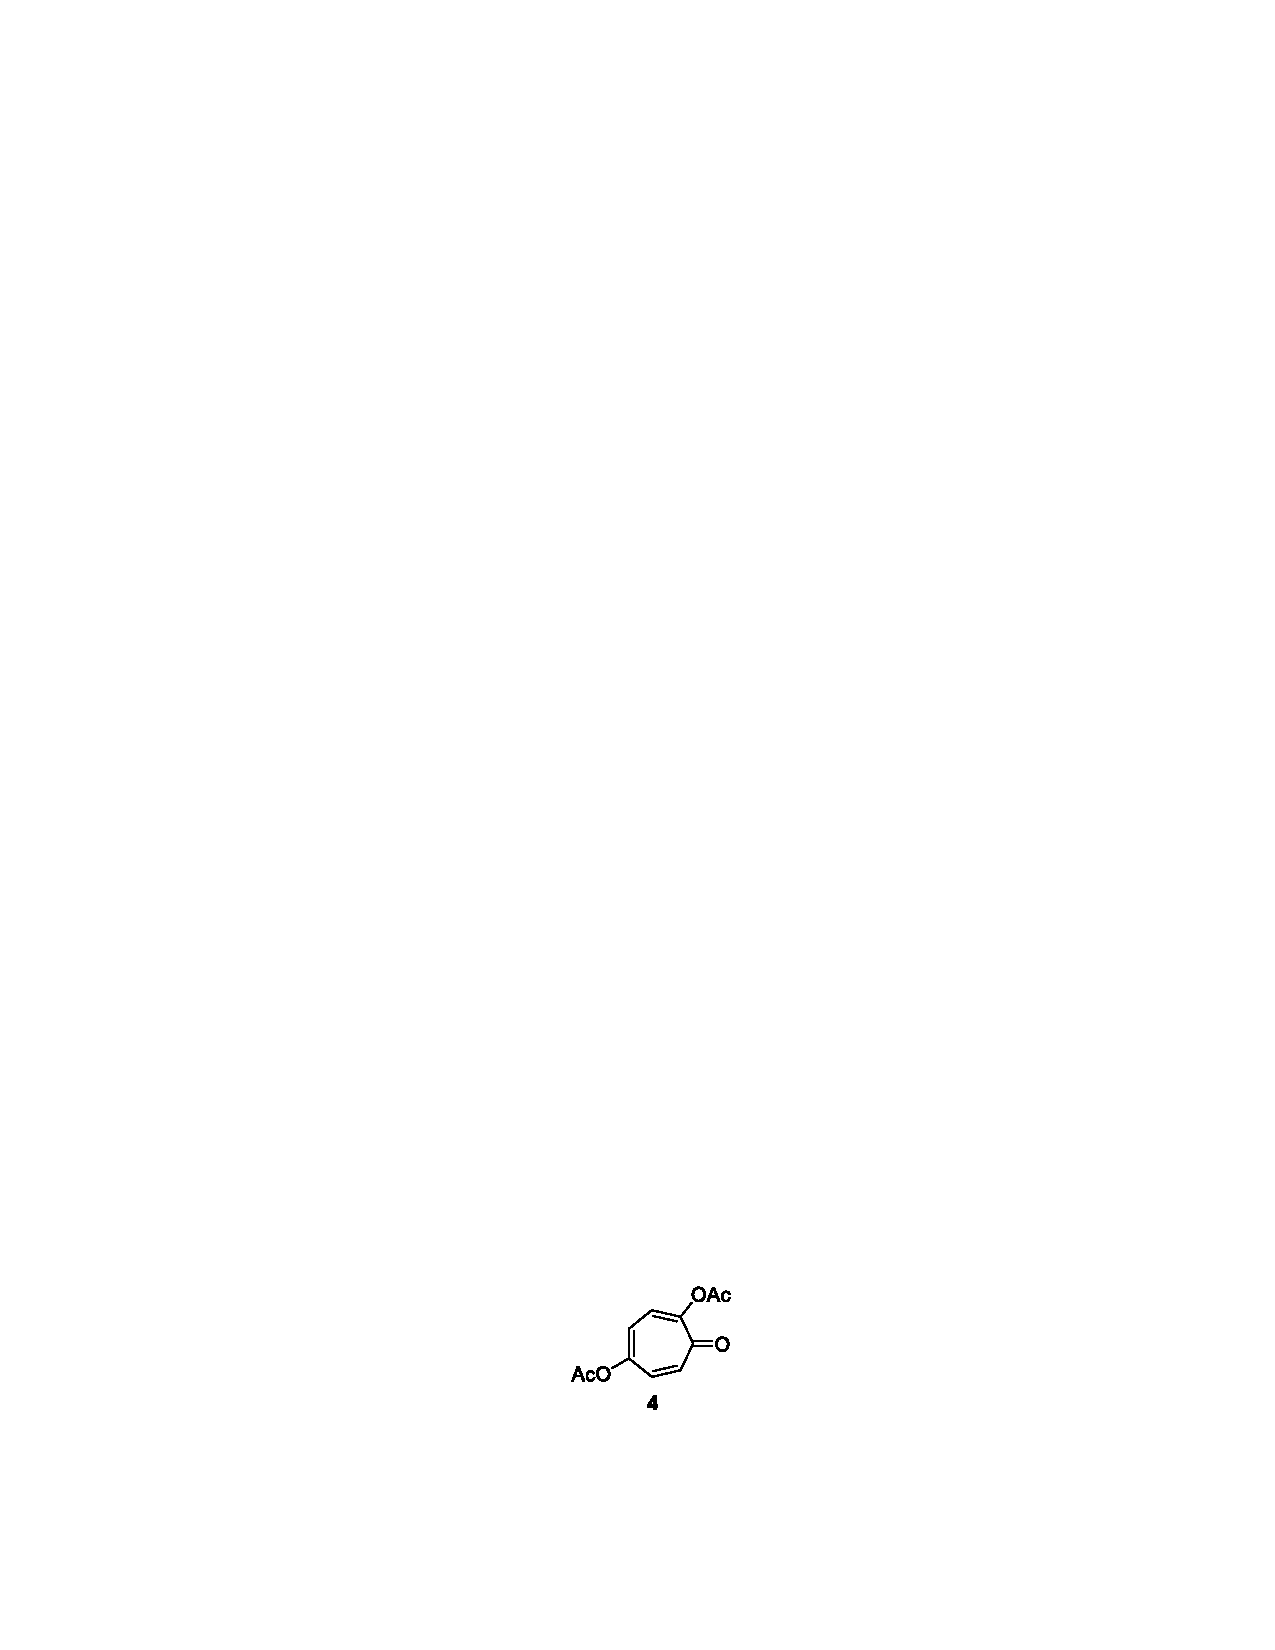
\includegraphics[width=5cm]{./pic/t9-4.pdf}
\end{figure}

\paragraph{双环(桥环)烯烃环氧化的立体化学}

\noindent\textbf{9.8.}考虑以下信息,画出所有在给出的反应条件下可能生成的立体异构体。

\noindent\textbf{提示:A}和\textbf{B}是在\textsuperscript{13}C NMR谱中含有三个峰的异构体,\textbf{C}是在\textsuperscript{13}C NMR谱中含有四个峰的异构体。

\begin{figure}[h]
	\centering
	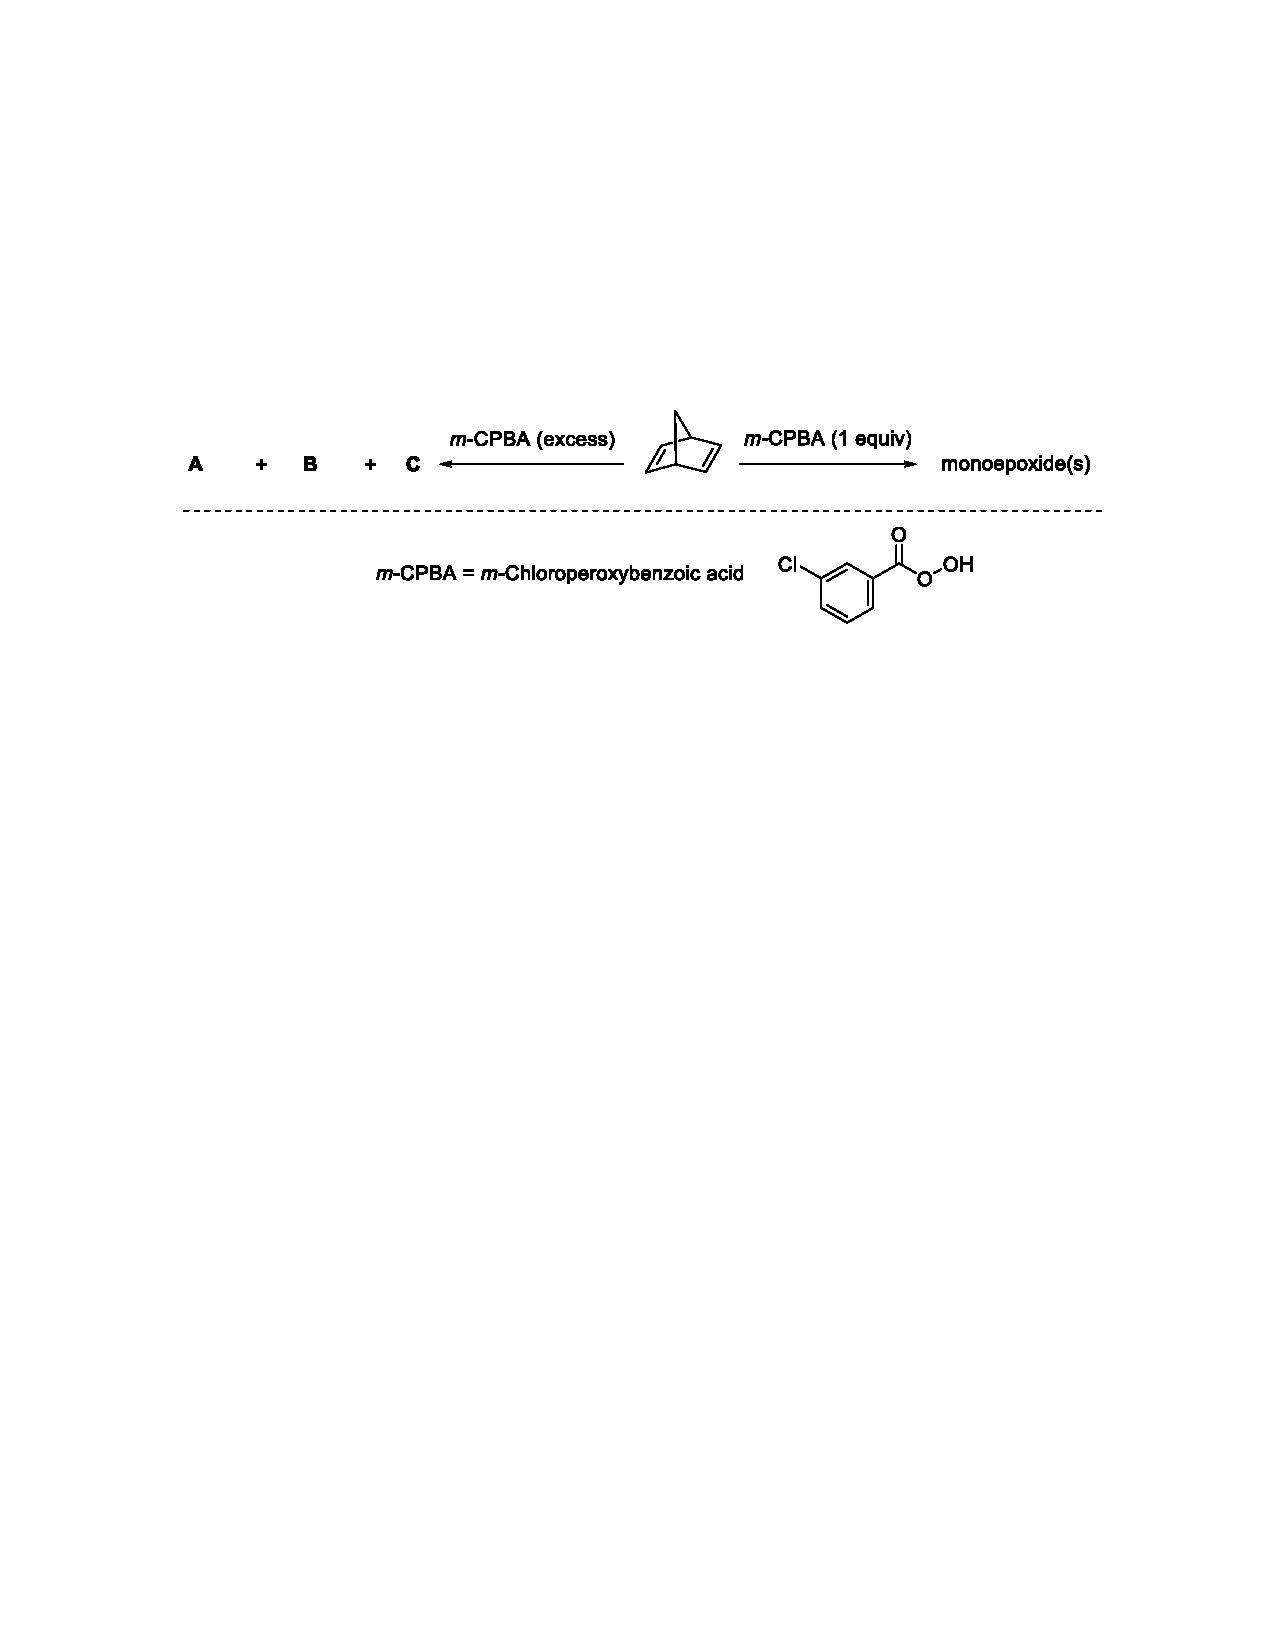
\includegraphics[width=14cm]{./pic/t9-5.pdf}
\end{figure}

\noindent\textbf{9.9.}
画出所有在给出的反应条件下可能生成的立体异构体。您认为在\textsuperscript{13}C
NMR谱中,各产物有多少个峰呢?

\begin{figure}[h!]
	\centering
	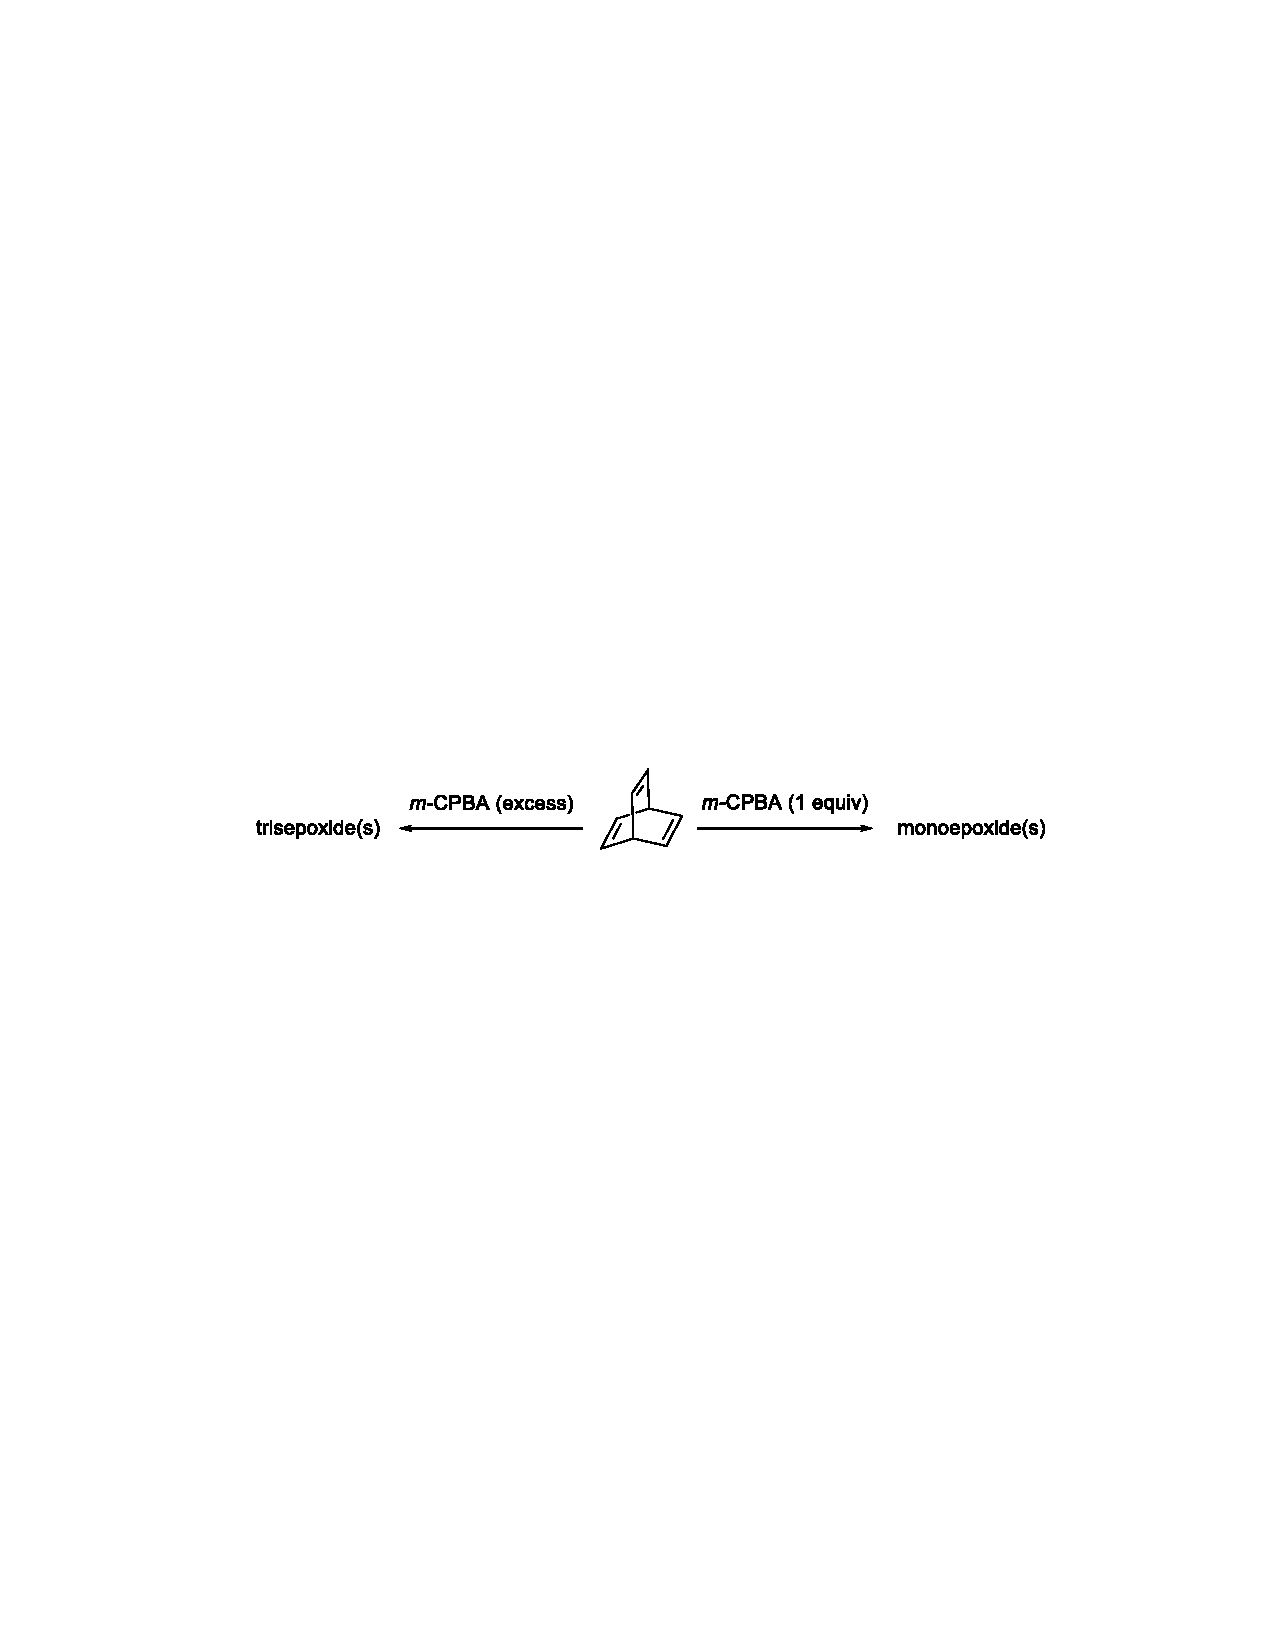
\includegraphics[width=11cm]{./pic/t9-6.pdf}
\end{figure}


\newpage
\mysection{第10题\  伍德沃德-霍夫曼规则与周环反应}
由Robert B. Woodward与Roald Hoffman提出的Woodward-Hoffman规则(即周环反应选择性规则)可被用于解释和预测周环反应的立体化学选择性及活化能,这一规则对于包括环加成反应、$\sigma$迁移反应、电环化反应及螯键反应的所有种类的周环反应(及它们的逆过程)都适用。

\begin{longtable}[]{@{}lll@{}}
	\toprule
	\textbf{系统} & \textbf{条件} & \textbf{移动}\tabularnewline
	\midrule
	4\emph{n} & 热($\Delta$) & 顺旋(con)\tabularnewline
	& 光($h\nu$) & 对旋(dis)\tabularnewline
	\midrule
	4\emph{n}+2 & 热 & 对旋\tabularnewline
	& 光 & 顺旋\tabularnewline
	\bottomrule
\end{longtable}

\begin{figure}[h]
	\centering
	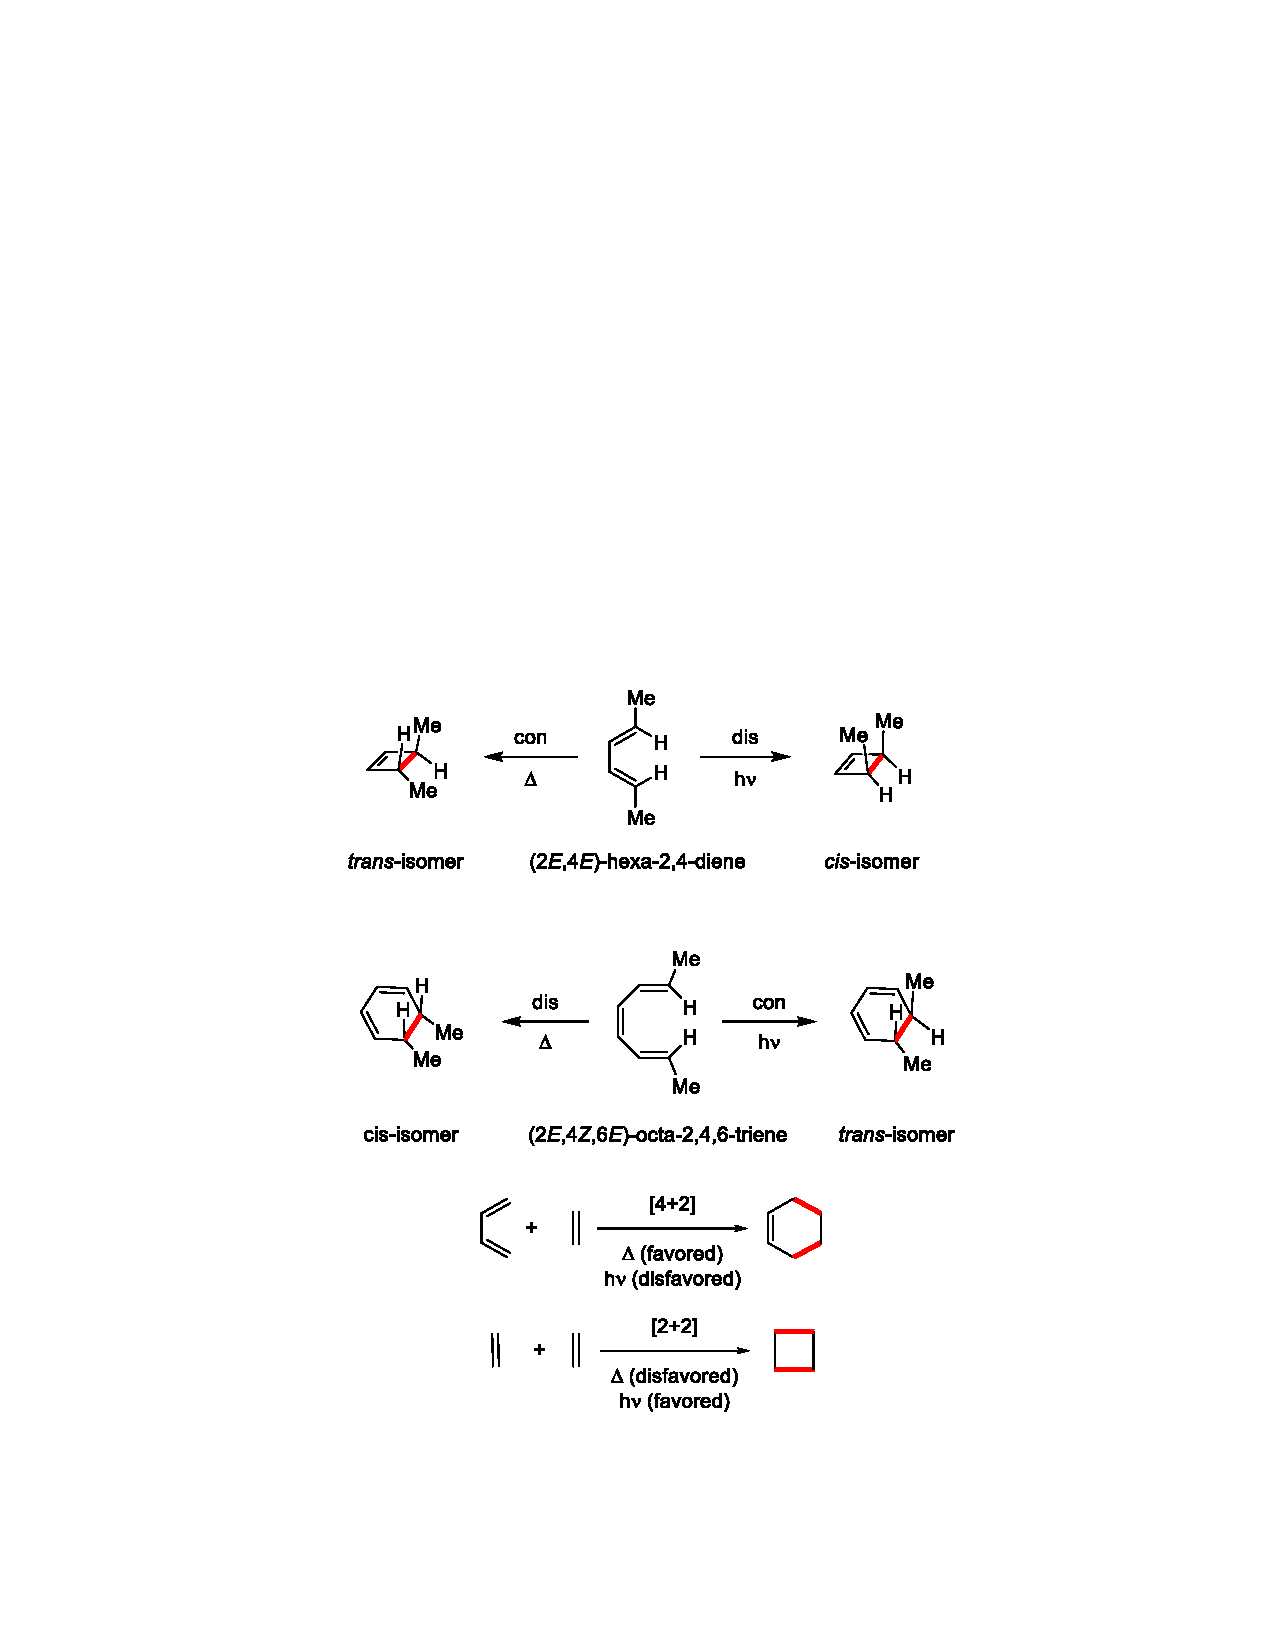
\includegraphics[width=10cm]{./pic/t10-1.pdf}
\end{figure}

\noindent\textbf{10.1.}
化合物\textbf{1}在加热下经一系列环加成反应得到土楠酸\textbf{2},结构如下所示。画出反应的具体步骤并对其中涉及的电环化反应进行分类。

\begin{figure}[h]
	\centering
	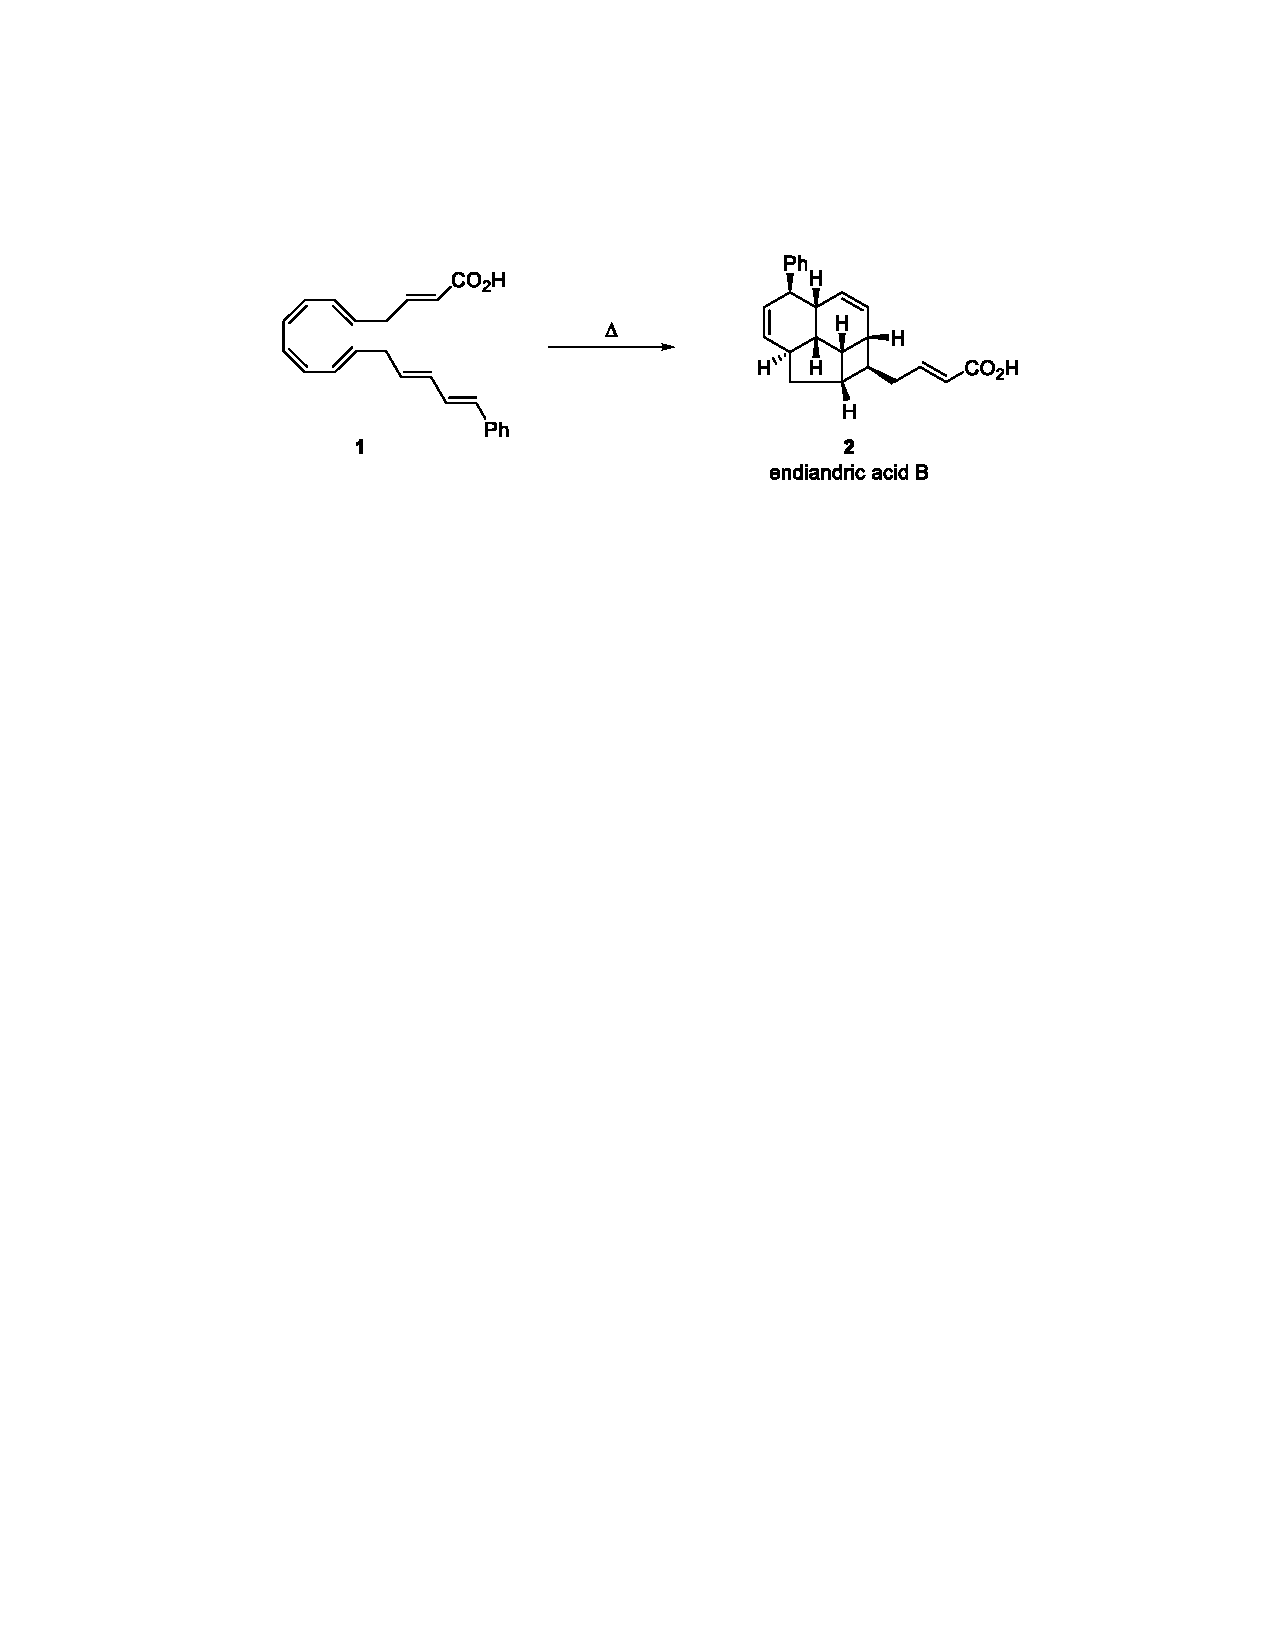
\includegraphics[width=12cm]{./pic/t10-2.pdf}
\end{figure}

在以下两小问的反应中,分别有多少$\pi$电子参与?根据Woodward-Hoffmann规则,这些反应的条件为光照还是加热?

\noindent\textbf{10.2.}

\begin{figure}[h]
	\centering
	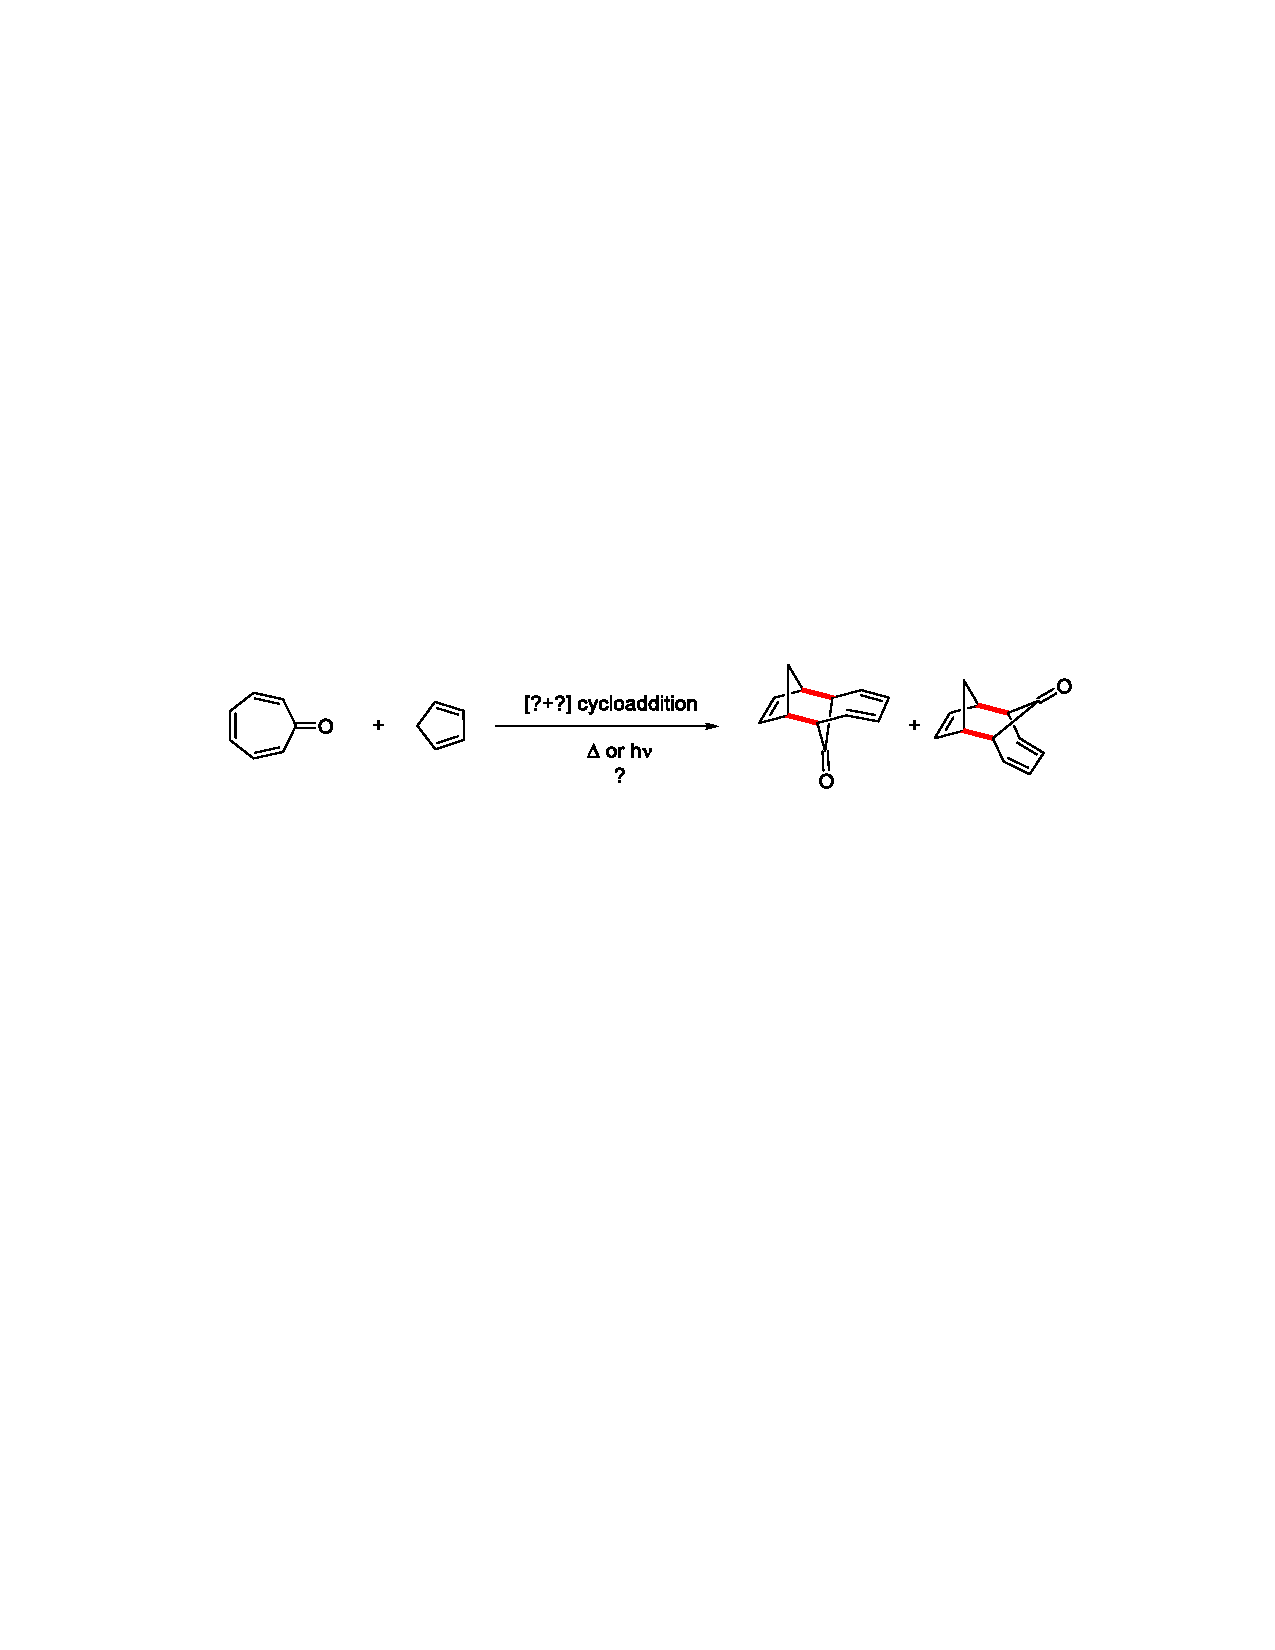
\includegraphics[width=13cm]{./pic/t10-3.pdf}
\end{figure}

\noindent\textbf{10.3.}

\begin{figure}[h]
	\centering
	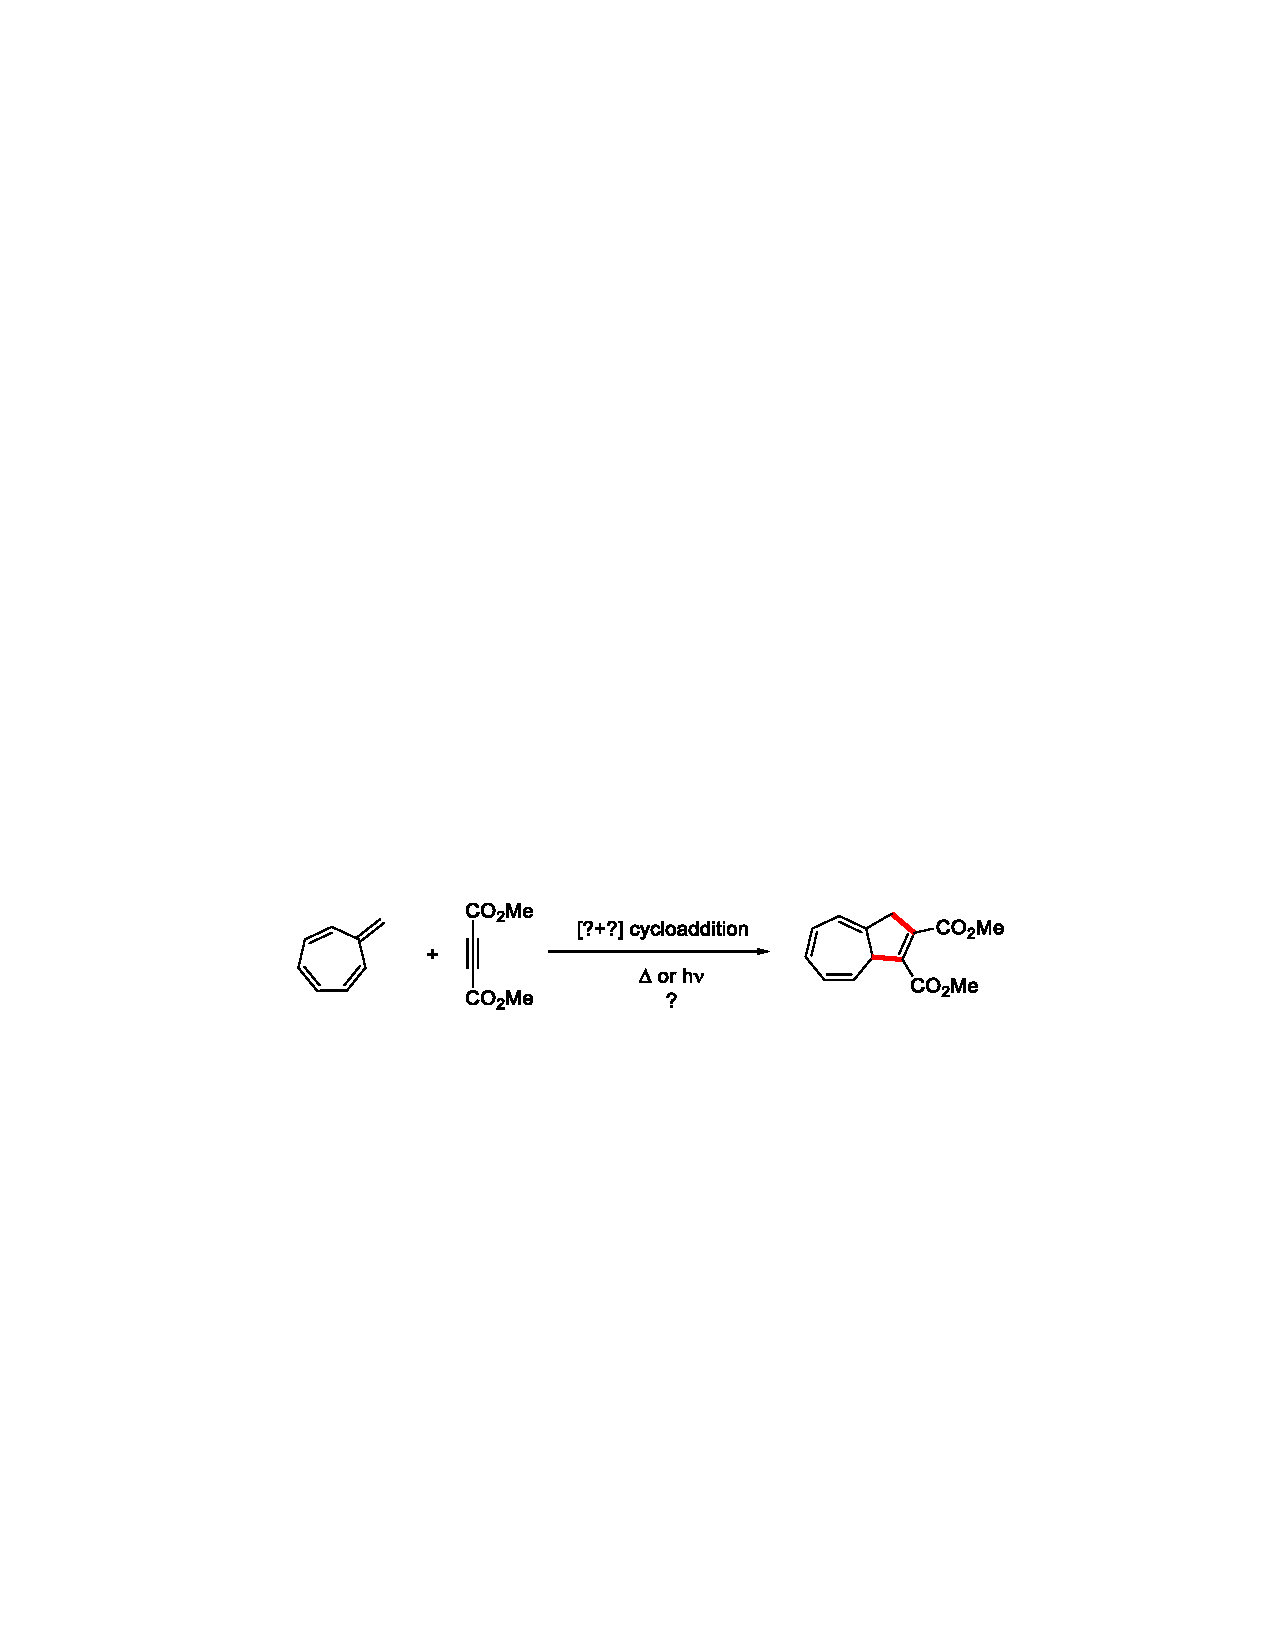
\includegraphics[width=12cm]{./pic/t10-4.pdf}
\end{figure}

\noindent\textbf{10.4.}
\textbf{A}与琥珀酰亚胺可以经连续的Diels-Alder反应生成化合物\textbf{3}。画出化合物\textbf{A}-\textbf{C}的结构。

\begin{figure}[h]
	\centering
	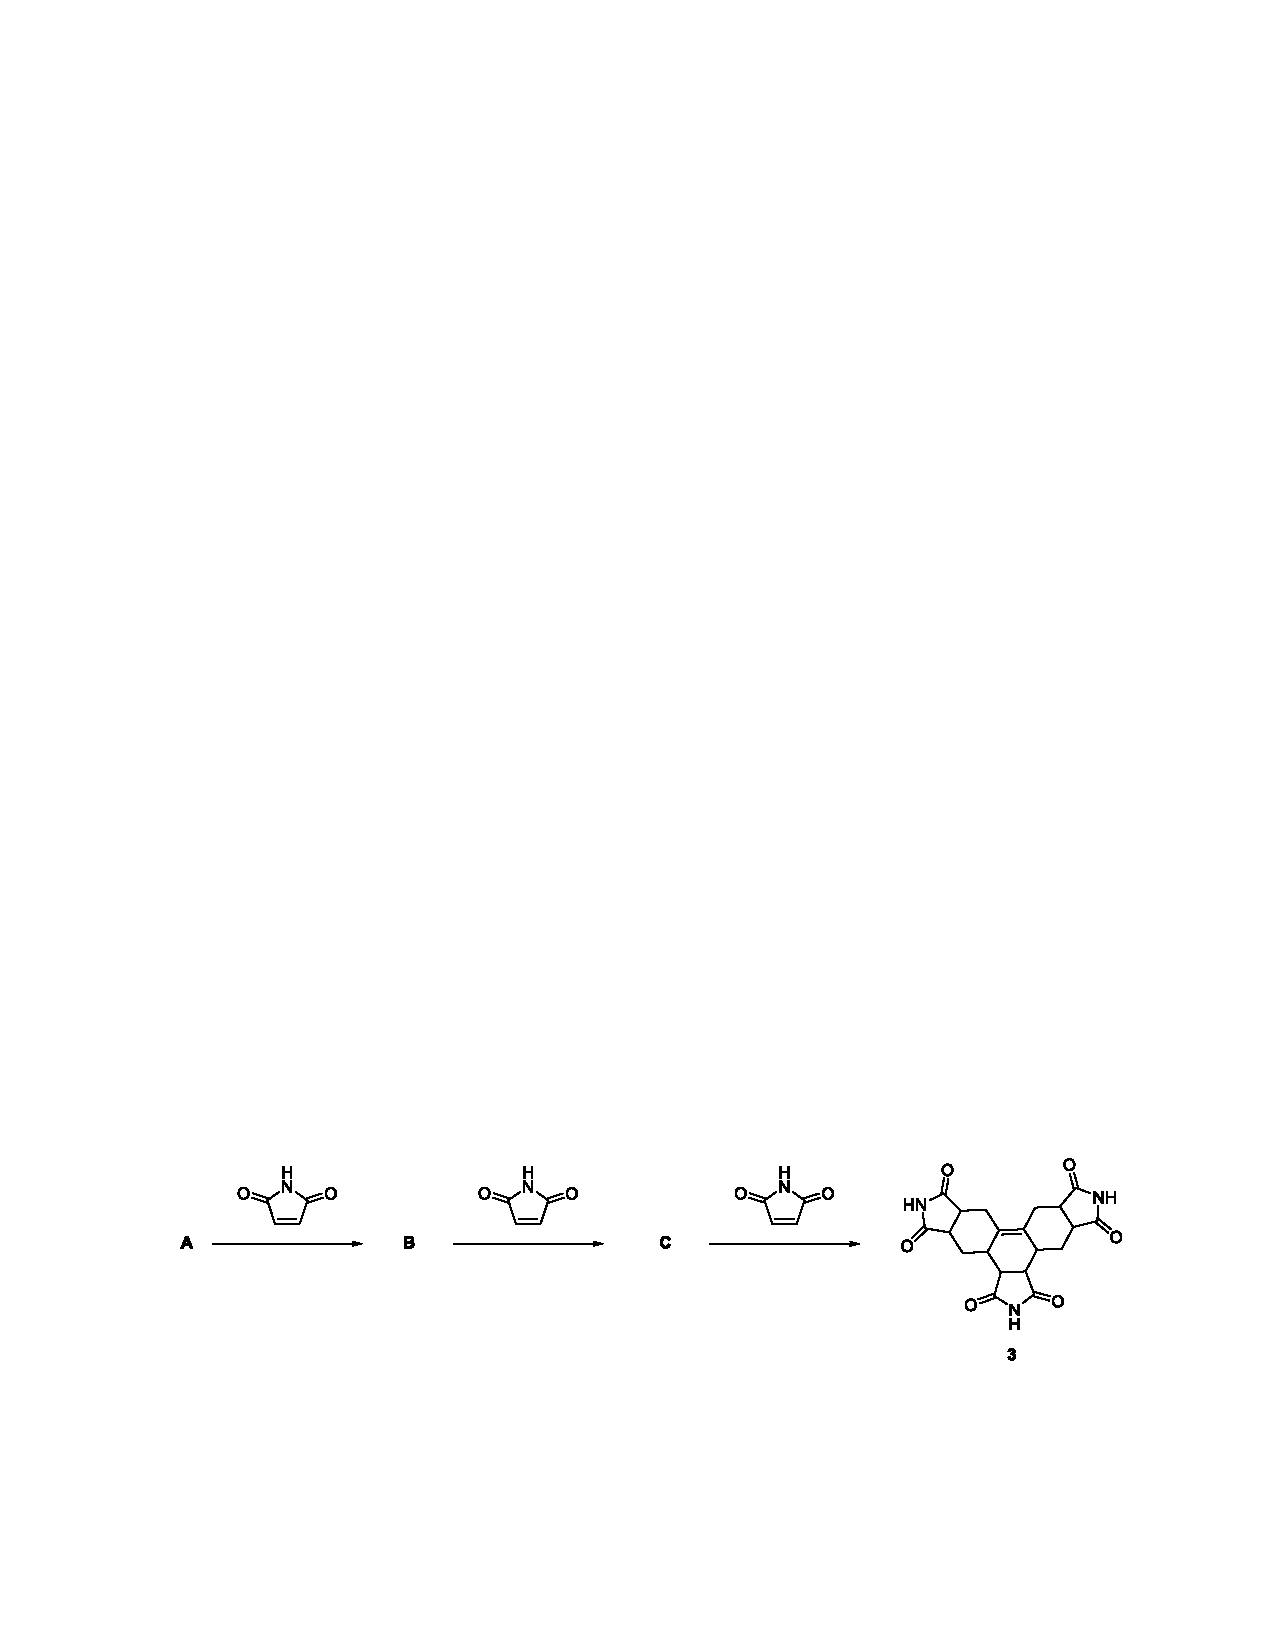
\includegraphics[width=16cm]{./pic/t10-5.pdf}
\end{figure}

\noindent\textbf{10.5.}
下面的反应路径图展示了从邻二甲苯开始合成苯系四环烃\textbf{I}的内式异构体的方法。用四溴代邻二甲苯\textbf{D}与碘化钠进行Br\textsubscript{2}消除反应,产生一个活性中间体\textbf{E},再经历一个4$\pi$电环化获得化合物\textbf{F}。画出中间体和产物\textbf{D}-\textbf{I}的结构。

\begin{figure}[h!]
	\centering
	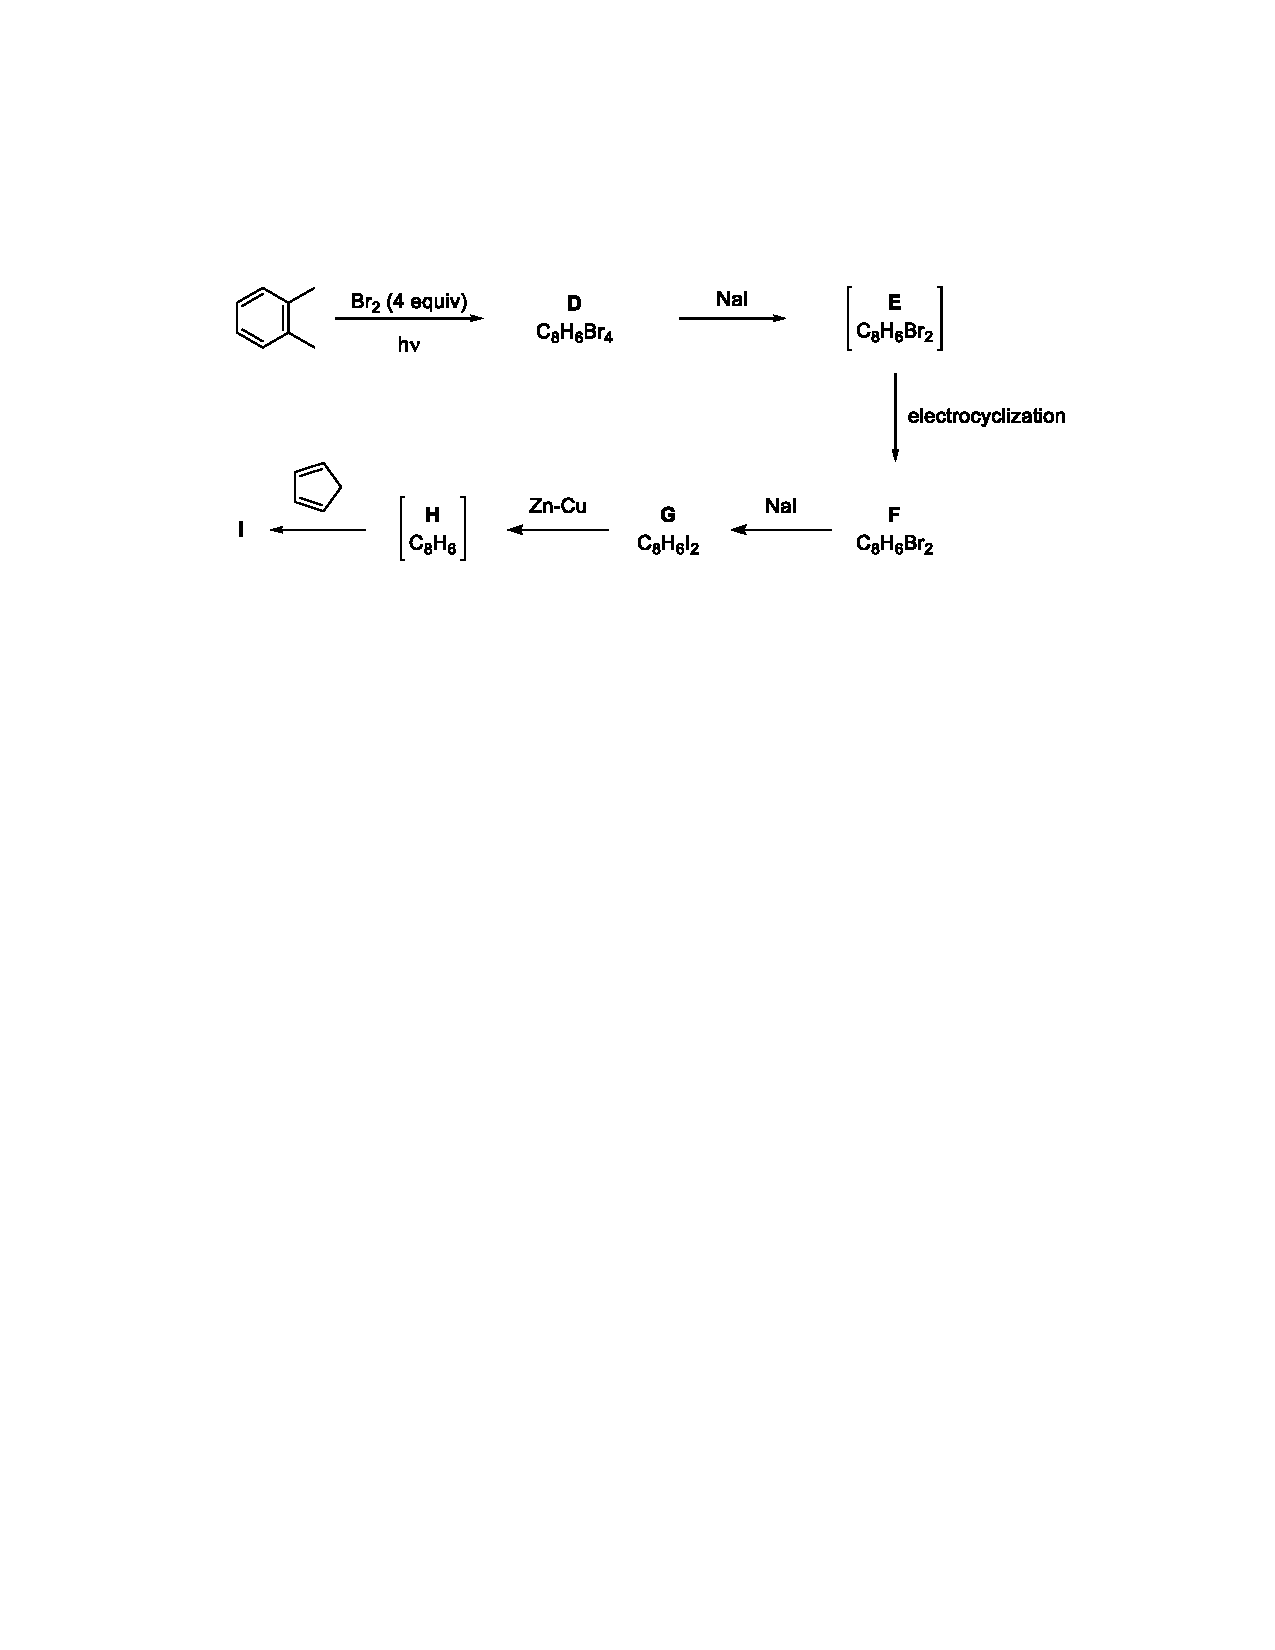
\includegraphics[width=12cm]{./pic/t10-6.pdf}
\end{figure}

\paragraph{逆Diels-Alder反应}

逆Diels-Alder反应是Diels-Alder反应的逆反应,环己烯衍生物分解为二烯及亲双烯体的反应便是一例。一般而言,逆Diels-Alder反应由热引发,但在某些情况下,由于底物性质不同,低温更利于反应的进行。

在有机化学、配位化学中,环戊二烯是常用的合成中间体,未取代的环戊二烯由二环戊二烯的分解反应制得。然而,由于顺式双键易迁移的特点,取代的环戊二烯并不稳定,因此制备取代的环戊二烯的方法十分有限。在下面的反应路径中,展示了取代环戊二烯衍生物的合成方法,其中除了逆Diels-Alder反应,还有反Diels-Alder反应,即富电子的亲双烯体和缺电子的双烯体(如四嗪\textbf{4}),通过亲双烯体的HOMO与双烯体的LUMO的相互作用进行的环加成反应。

\noindent\textbf{10.6.} 画出中间体和产物\textbf{J-N}的结构。

\begin{figure}[h!]
	\centering
	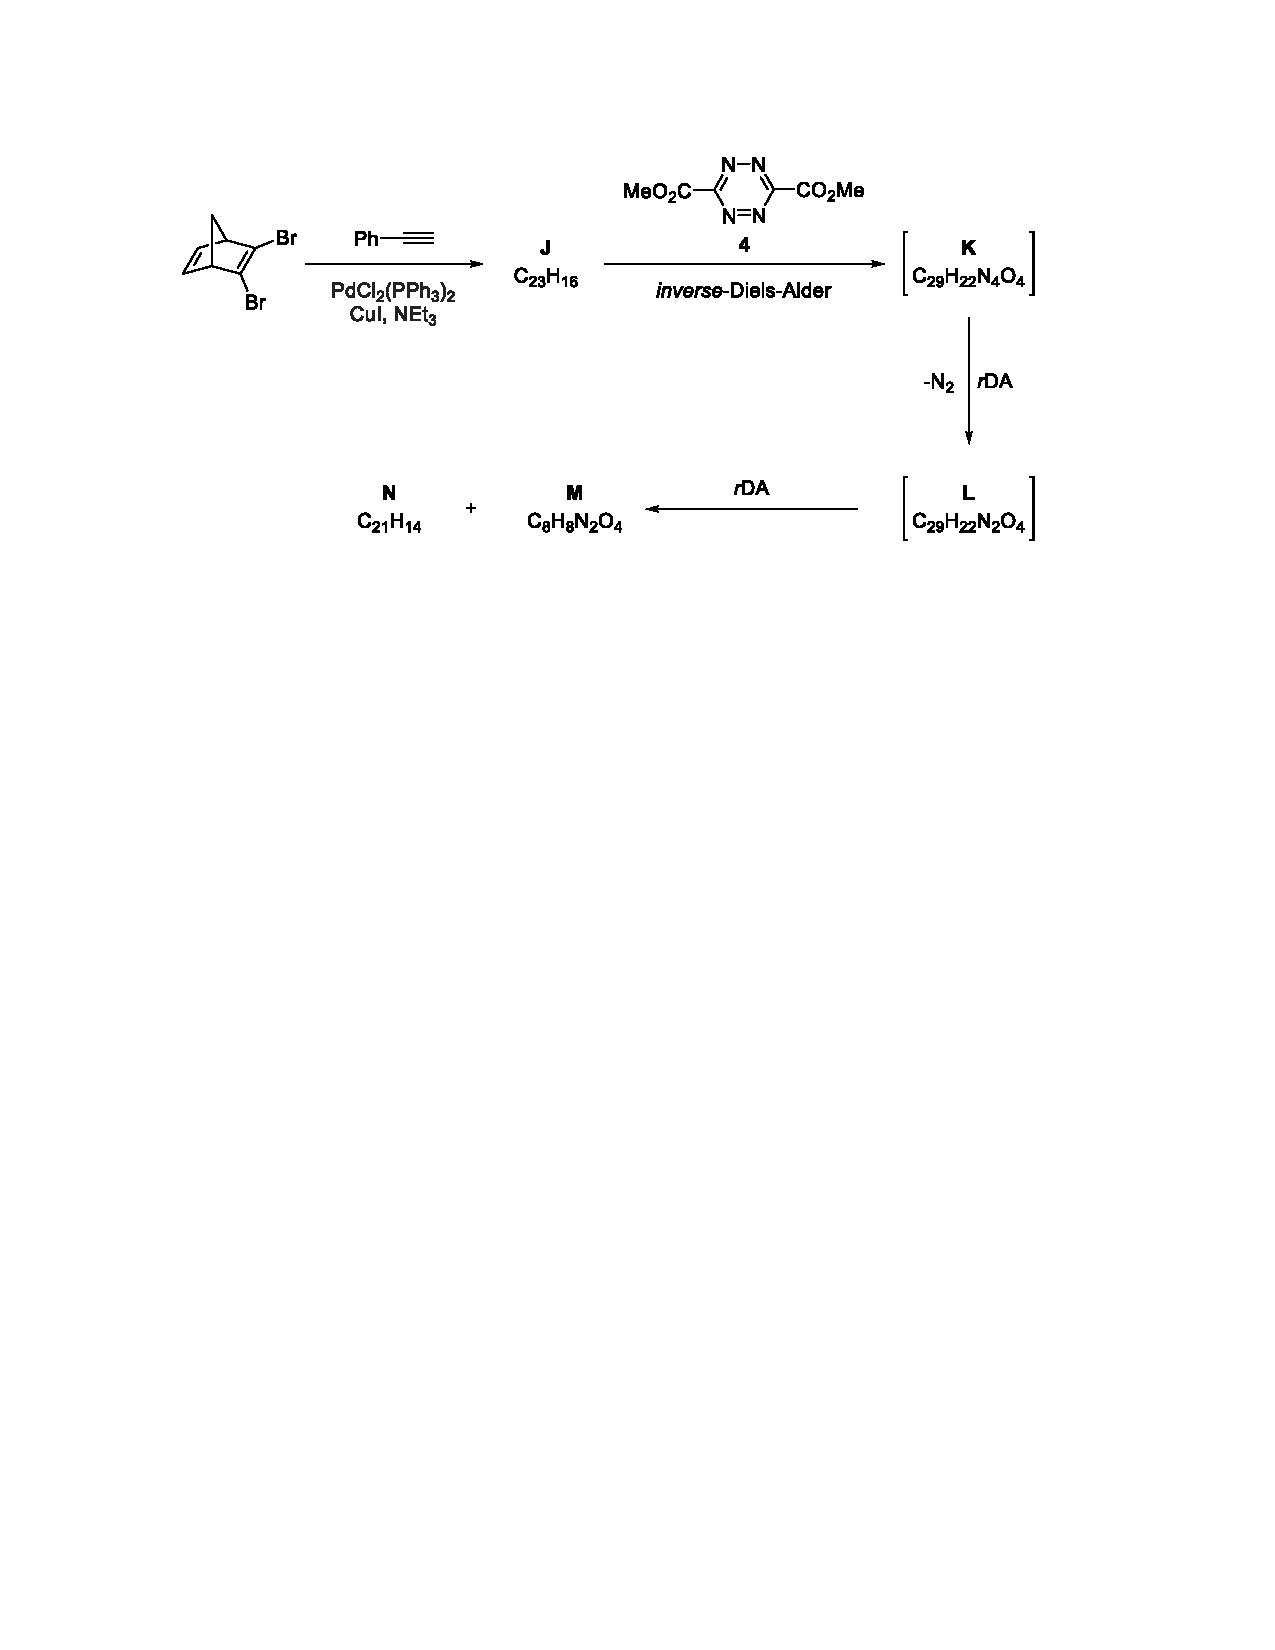
\includegraphics[width=13.5cm]{./pic/t10-7.pdf}
\end{figure}

\noindent\textbf{10.7.}
亲核芳香取代反应是有机合成化学中一类非常重要的反应。在下图中,两种不同结构的芳香卤化物\textbf{5}在不同的反应条件下进行反应,反应中经历了两种不同的中间体,这两种中间体具有环状1,3-二烯结构。画出两种产物(\textbf{O}和\textbf{P})的结构,讨论生成这两种产物过程中的可能中间体。

\begin{figure}[h!]
	\centering
	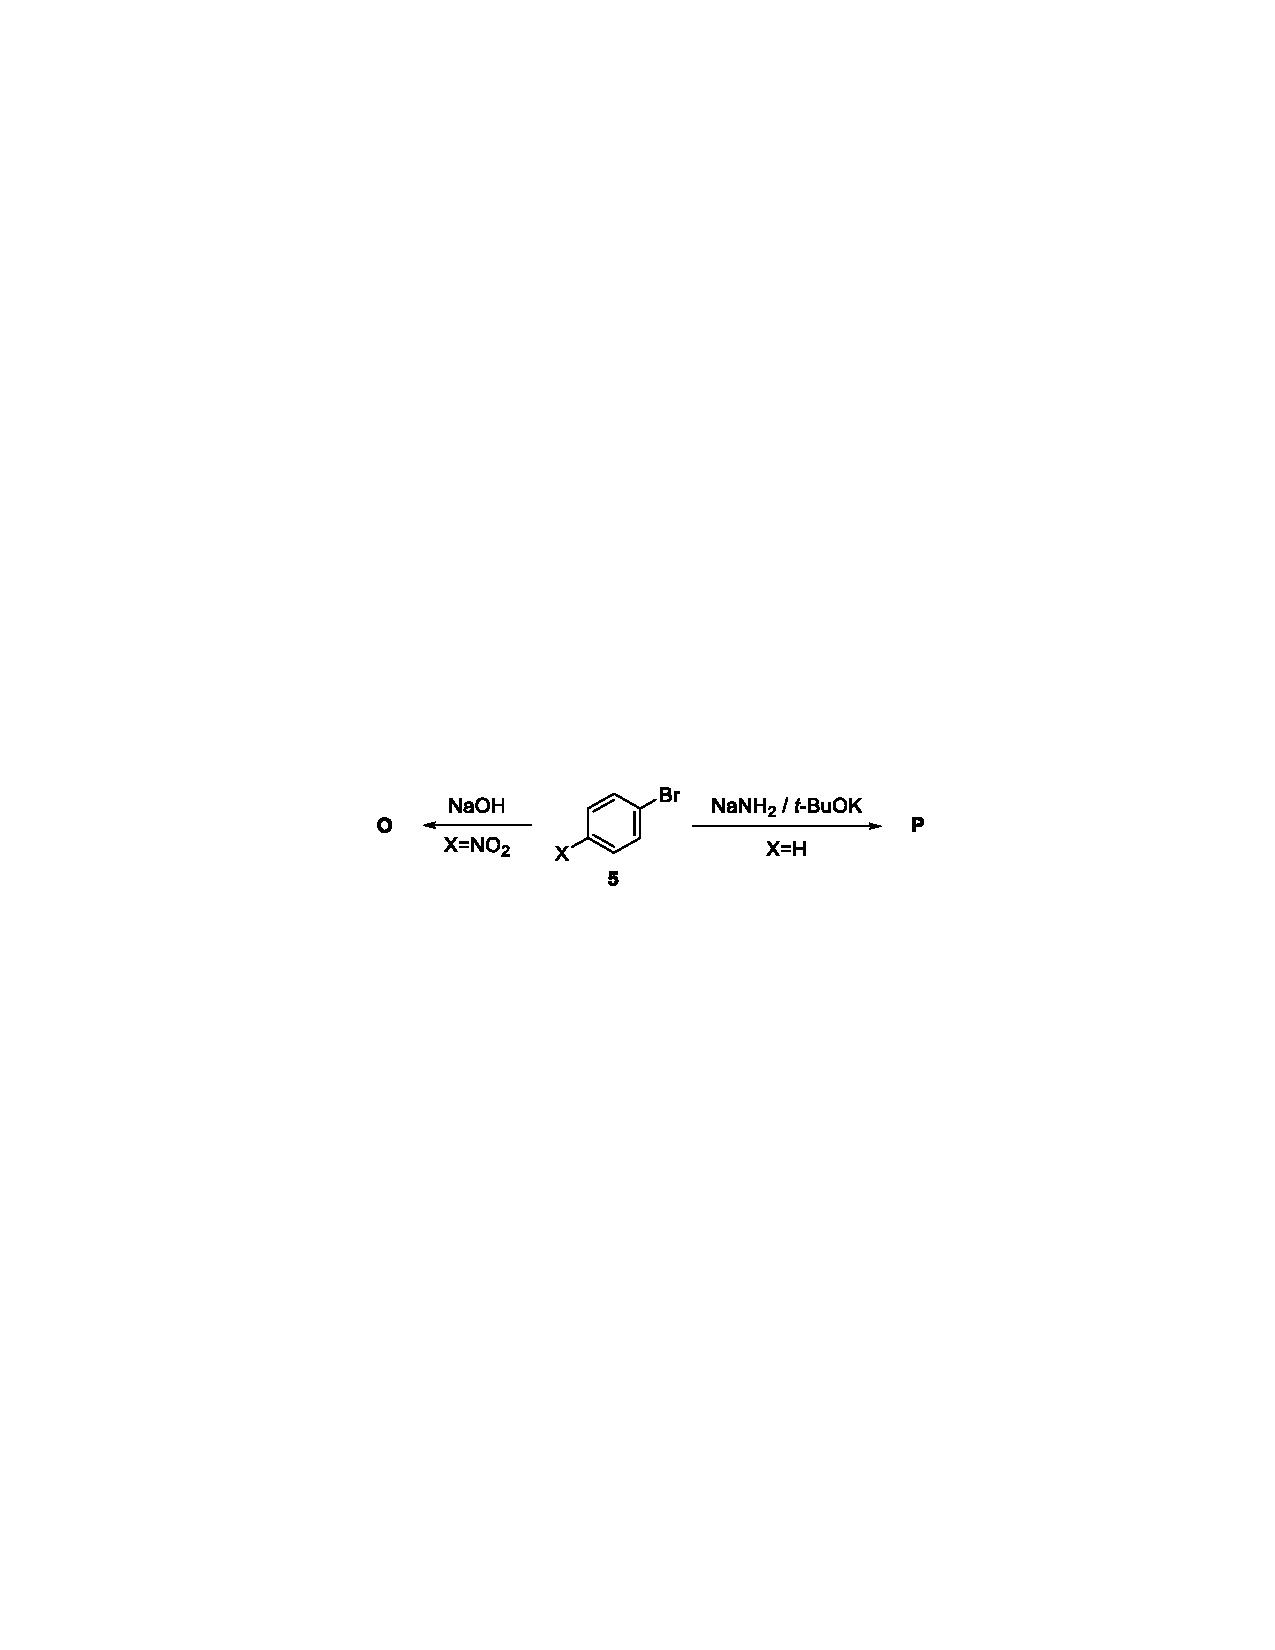
\includegraphics[width=8.5cm]{./pic/t10-8.pdf}
\end{figure}

\newpage
\mysection{第11题\  苯并卟啉}
卟啉的英文名``porphyrin''源自于古希腊词汇``\emph{porphyra}'',意为紫色。卟啉是一系列大环有机化合物的总称,其中包含四个被修饰的吡咯单元。卟啉共有26个π电子,其中18个构成了平面的卟啉环结构,常被认为具有芳香性。在自然界中,存在着卟啉与金属的配合物,其中最广为人知的一族卟啉配合物是红细胞色素,亚铁血红素。苯并卟啉由苯环与卟啉环中的吡咯单元邻接而成。

\begin{figure}[h!]
	\centering
	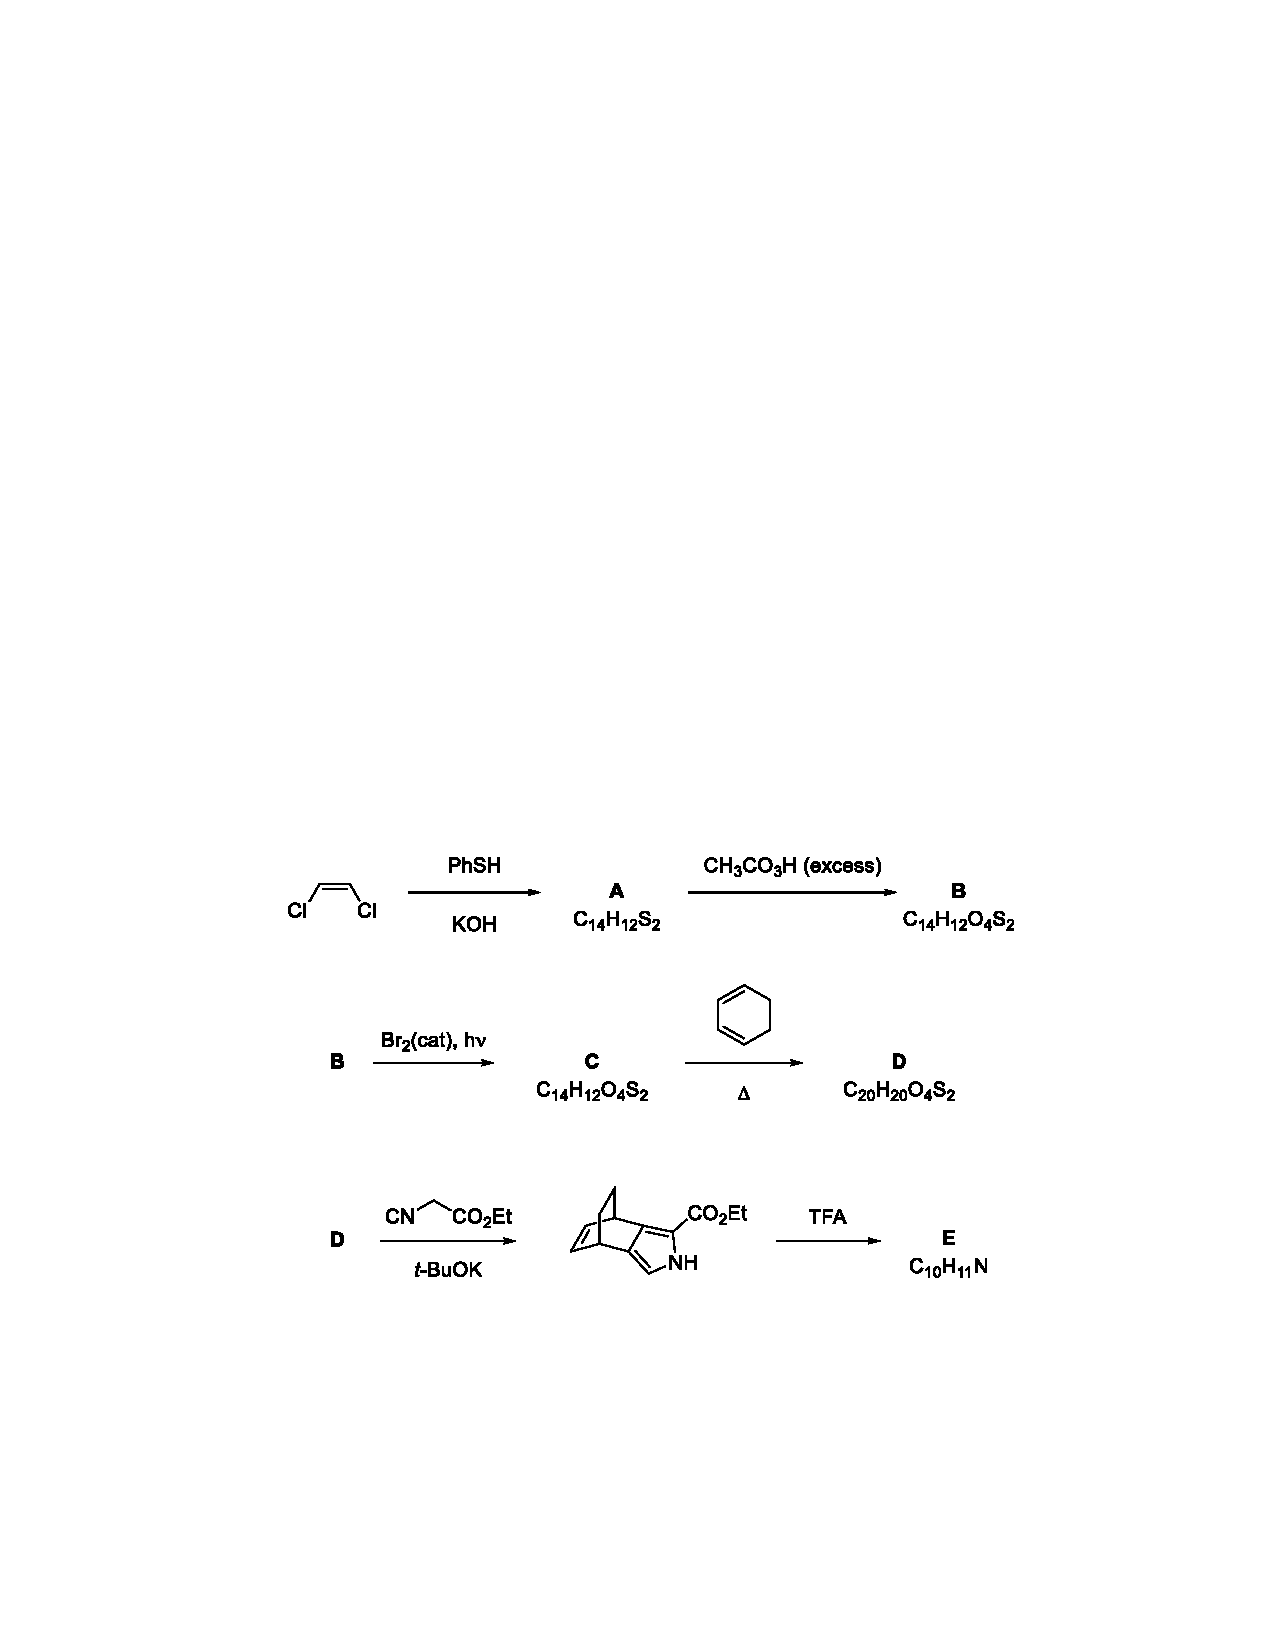
\includegraphics[width=11cm]{./pic/t11-1.pdf}
\end{figure}

苯并卟啉可以由吡咯衍生物\textbf{E}制备,上面的合成路线展示了化合物\textbf{E}的制备方法。首先,反式1,2-二氯乙烯与苯硫酚反应生成化合物\textbf{A},化合物\textbf{A}经氧化生成化合物\textbf{B},化合物\textbf{B}带有苯磺酰单元。顺式化合物\textbf{B}在紫外光照射下经催化量的Br\textsubscript{2}处理转化为其反式异构体\textbf{C},\textbf{C}与1,3-环己二烯在加热条件下发生Diels-Alder反应得到化合物\textbf{D}。化合物\textbf{D}与异氰基乙酸乙酯反应生成一种吡咯甲酸酯衍生物,其与TFA反应生成吡咯衍生物\textbf{E}。

\begin{figure}[h!]
	\centering
	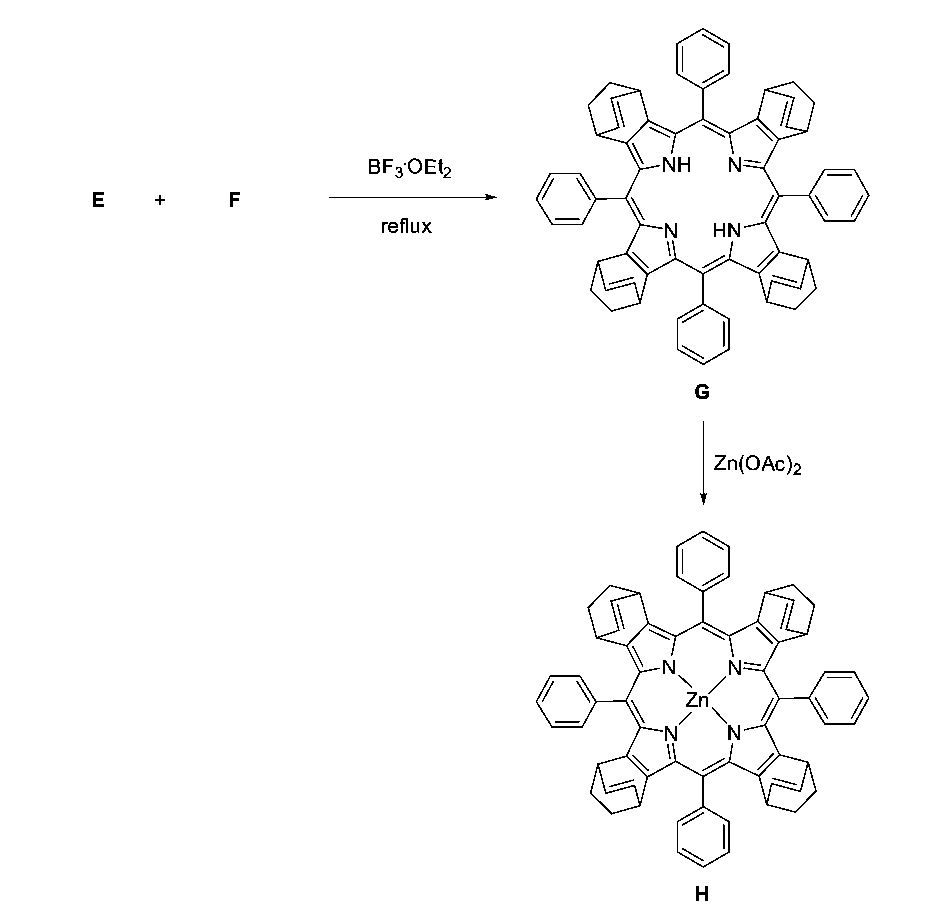
\includegraphics[width=12cm]{./pic/t11-2.pdf}
\end{figure}

\noindent\textbf{11.1.}画出化合物\textbf{A-E}的结构,必要时需表示出立体化学。

\noindent\textbf{11.2.}
卟啉可由吡咯衍生物与醛类化合物经环化反应制备。画出醛类化合物\textbf{F}的结构,写出化合物\textbf{H}中锌的氧化态。

将化合物\textbf{H}在真空中加热,它会发生逆Diels-Alder反应,生成一个共轭体系更大的化合物。

\noindent\textbf{11.3.} 在虚线圆圈内画出化合物\textbf{I}不全的部分,画出化合物\textbf{J}。

\begin{figure}[h]
	\centering
	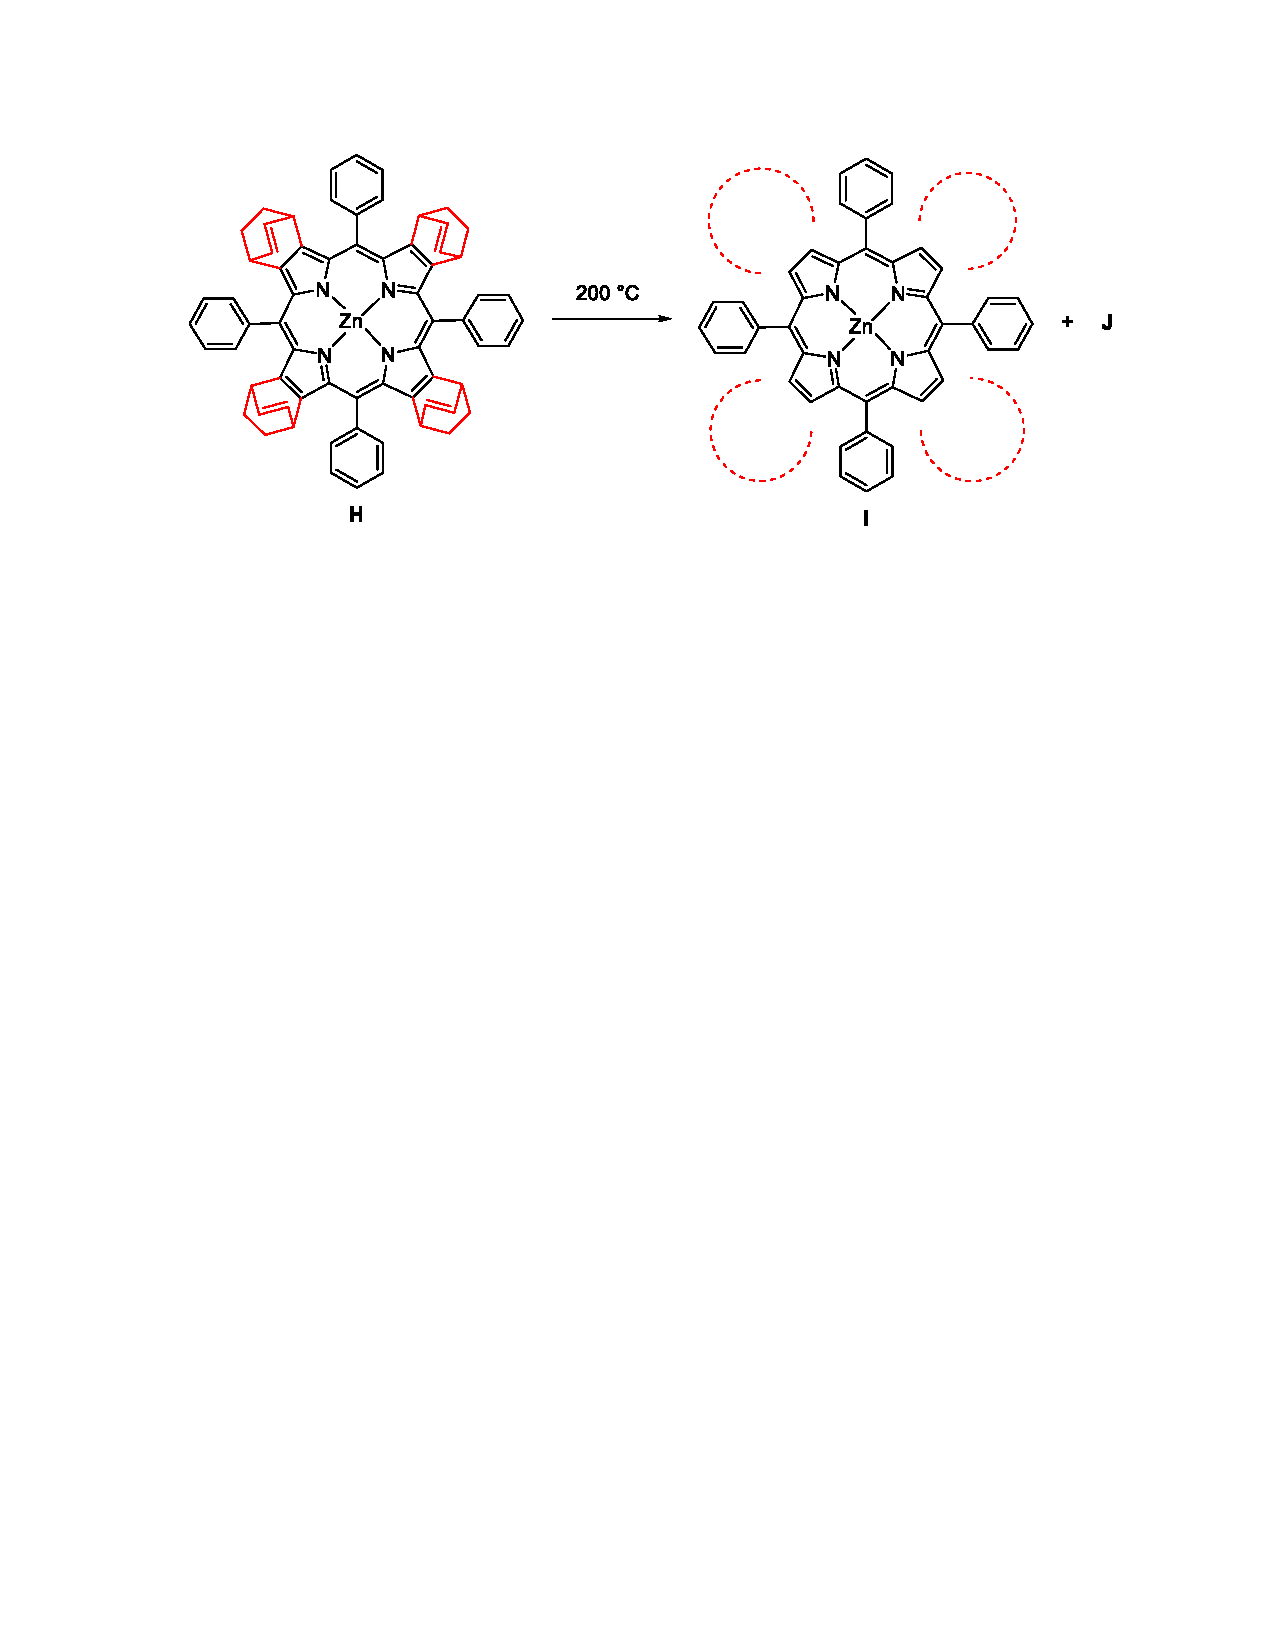
\includegraphics[width=13cm]{./pic/t11-3.pdf}
\end{figure}

氨是一种重要的参与新陈代谢的分子,由于其与某些特定疾病有关,关于如何灵敏而准确地测定其浓度的研究近来十分受重视。在正常生理条件下,弱碱性血液中的氨可通过皮肤或呼吸排出。肝脏、肾脏可将氨转化为尿素,在这两个器官功能紊乱时,呼吸和尿液中的氨浓度会升高,因此对呼吸和尿液中氨浓度的探测可作为鉴定早期肝脏和胃部疾病的指标。要达到此目标,需要发展灵敏度在50 ppb-2 ppm,响应迅速的测量传感器。

为此,化合物\textbf{I}被用于光纤氨分子探测传感器,氨分子能改变这种光纤的透光率。将不同浓度的氨气通过探测器,使用合适的光谱探测透光率的变化,结果列于下表。

\begin{figure}[h]
	\centering
	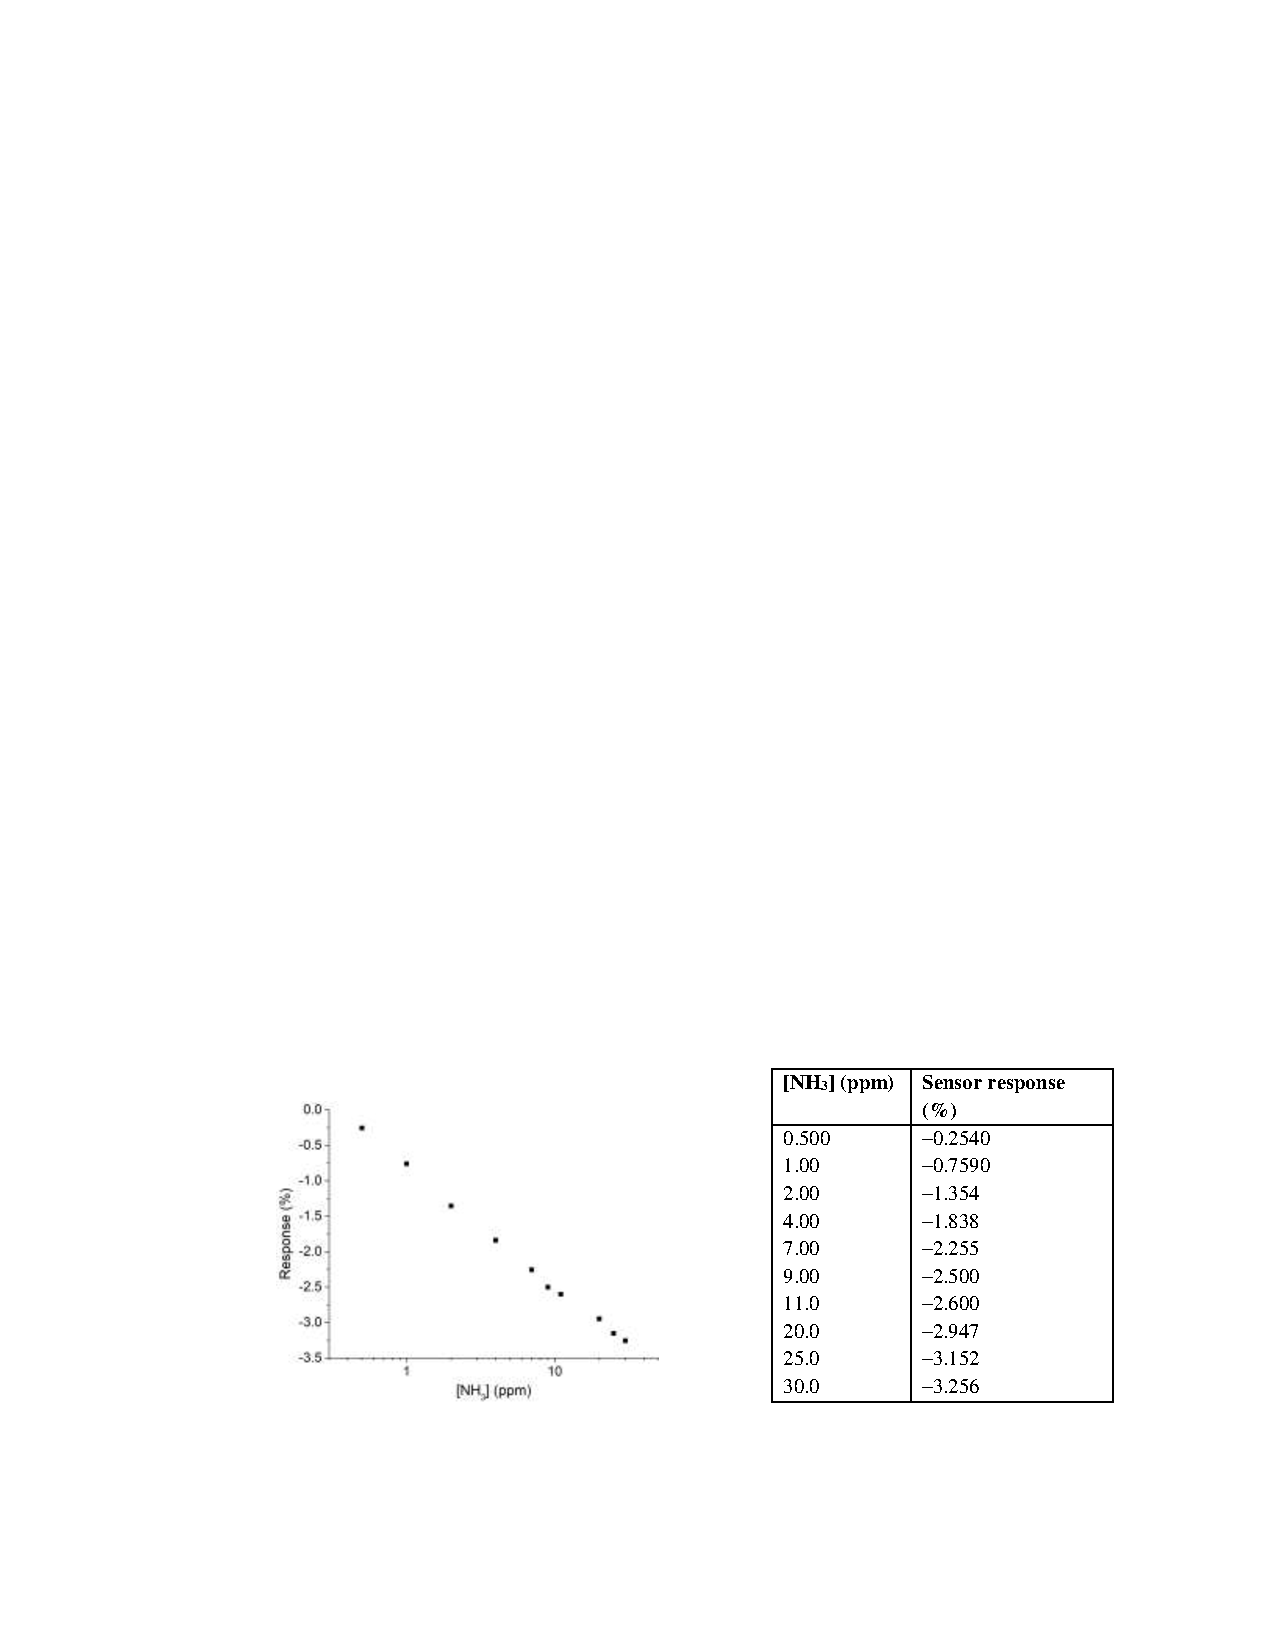
\includegraphics[width=14cm]{./pic/t11-4.pdf}
\end{figure}

\noindent\textbf{11.4.} 在探测器测得数据的线性区域作一条校准曲线,得到形如$y=a+bx$的校准曲线方程。

\noindent\textbf{11.5.}
用此探测器探测一肝脏疾病患者呼吸中的氨浓度,检测器检测到−3.812\%的信号变化。计算病人呼吸中的氨浓度。


\newpage
\mysection{第12题\  绿松石,蓝绿色}
在土耳其南方省份布尔杜尔的叶西洛娃区,碧蓝之色与洁白的沙滩交相辉映,绿松石色(蓝绿色)的湖水令来自全世界的游客流连忘返,这里就是久负盛名,有着``土耳其的马尔代夫''之称的萨尔达湖。绿松石是一种不透明、蓝绿色的铜铝混合磷酸盐水合物矿石,其化学组成为CuAl\textsubscript{6}(PO\textsubscript{4})\textsubscript{4}(OH)\textsubscript{8}·4H\textsubscript{2}O,绿松石也可作为宝石。绿松石一词最早来源于十七世纪的法语,意为``土耳其的'',其原因为绿松石最早是从曾经的波斯呼罗珊省经土耳其运入欧洲的。绿松石结构中的磷酸根是生命中不可缺少的一部分,它存在于维持生命所必需的ATP、ADP及DNA等化合物中,也可以在骨骼与牙齿的无机质中找到。自然界矿物中的磷酸盐几乎全部以最高氧化态存在,这些无机矿物部分由磷灰石组成,是商业上磷元素的主要来源。在农业上,磷酸盐可用作肥料、作为发酵粉和面粉的膨松剂、饮料的添加剂,并且在饲养动物和医药上也有应用。在工业上,磷酸盐可用于水质软化、防火、防锈、杀虫剂和清洁剂以及单质磷的生产。

\begin{figure}[h]
	\centering
	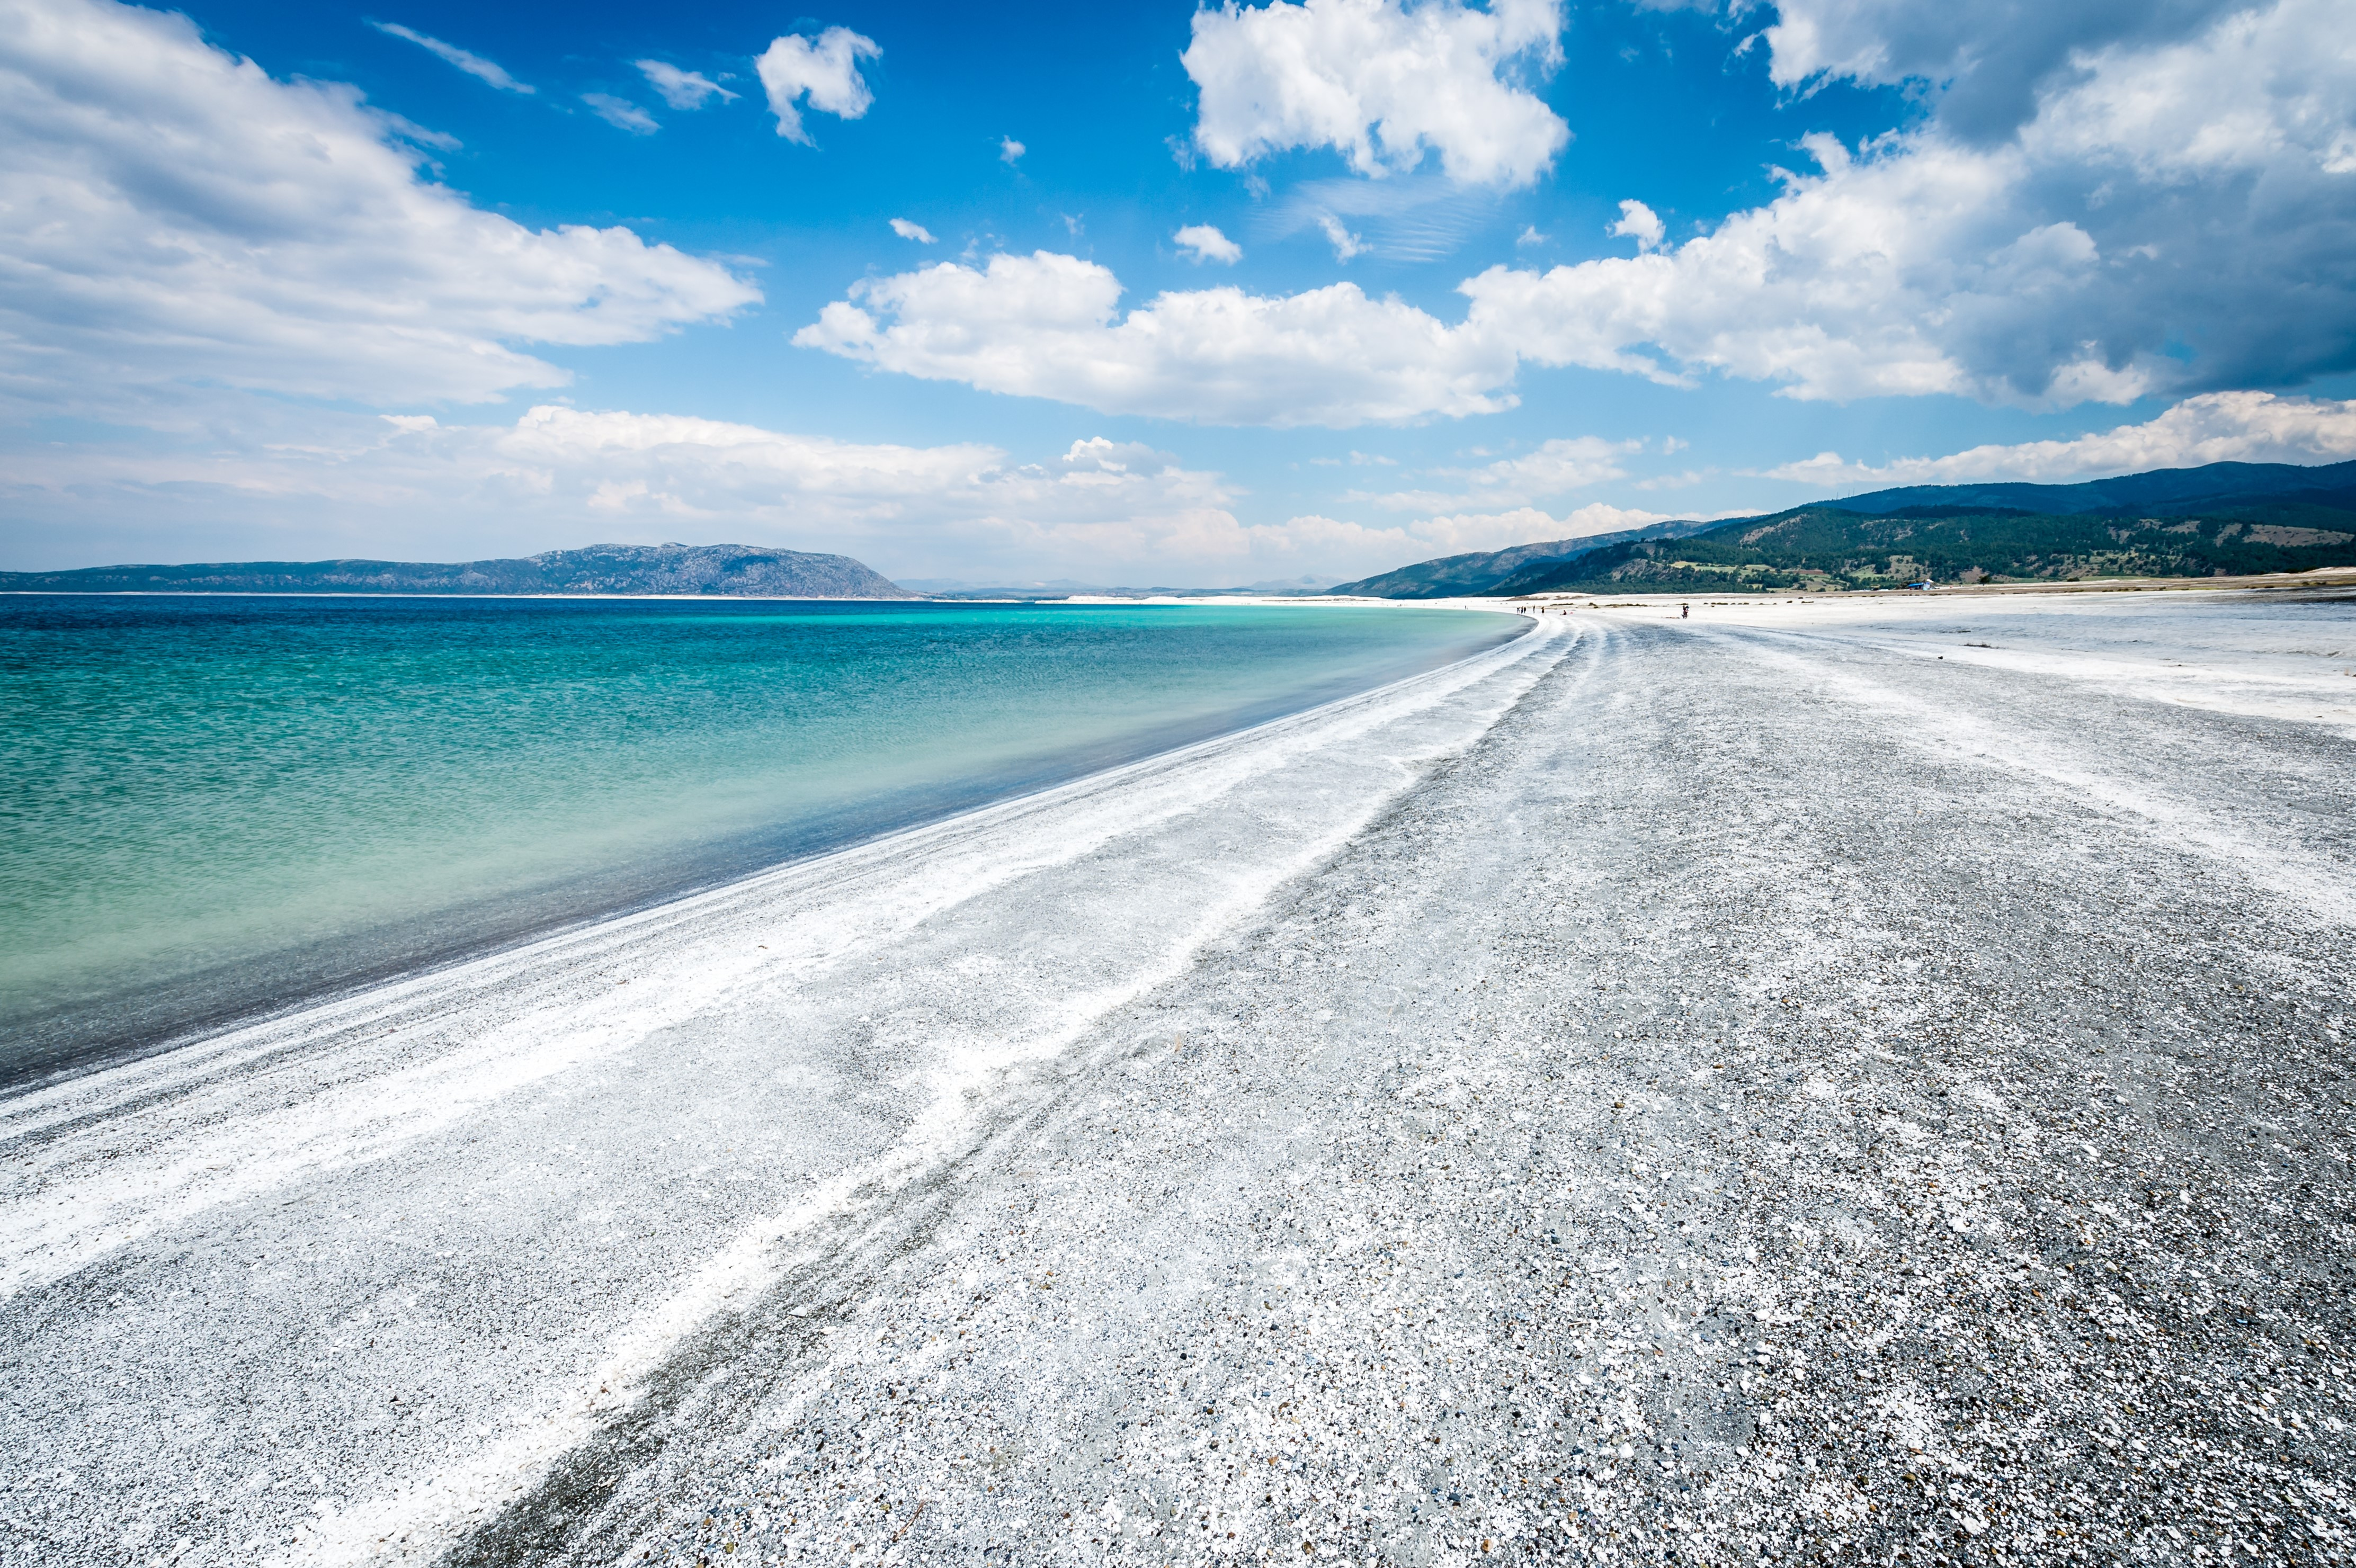
\includegraphics[width=10cm]{./pic/t12-1.jpg}
	\caption*{萨尔达湖}
\end{figure}

磷有三种重要同素异形体:\textbf{X}、\textbf{Y}和\textbf{Z}。除此之外,还存在一种同素异形体\textbf{W}。\textbf{X}是一种很软、白色的固体,它化学性质活泼,有毒害并可表现出化学发光的性质。\textbf{X}的晶体中包含P\textsubscript{4}分子。将\textbf{X}在黑暗中加热至250 °C可得到\textbf{Y},它无毒无味,且不具有化学发光的性质,为固体聚合物结构。\textbf{Z}可由\textbf{X}在惰性气氛中转变得到,它最为稳定,具有层状结构。\textbf{W}可由\textbf{Y}在550 °C以上退火数日得到。

\begin{figure}[H]
	\centering
	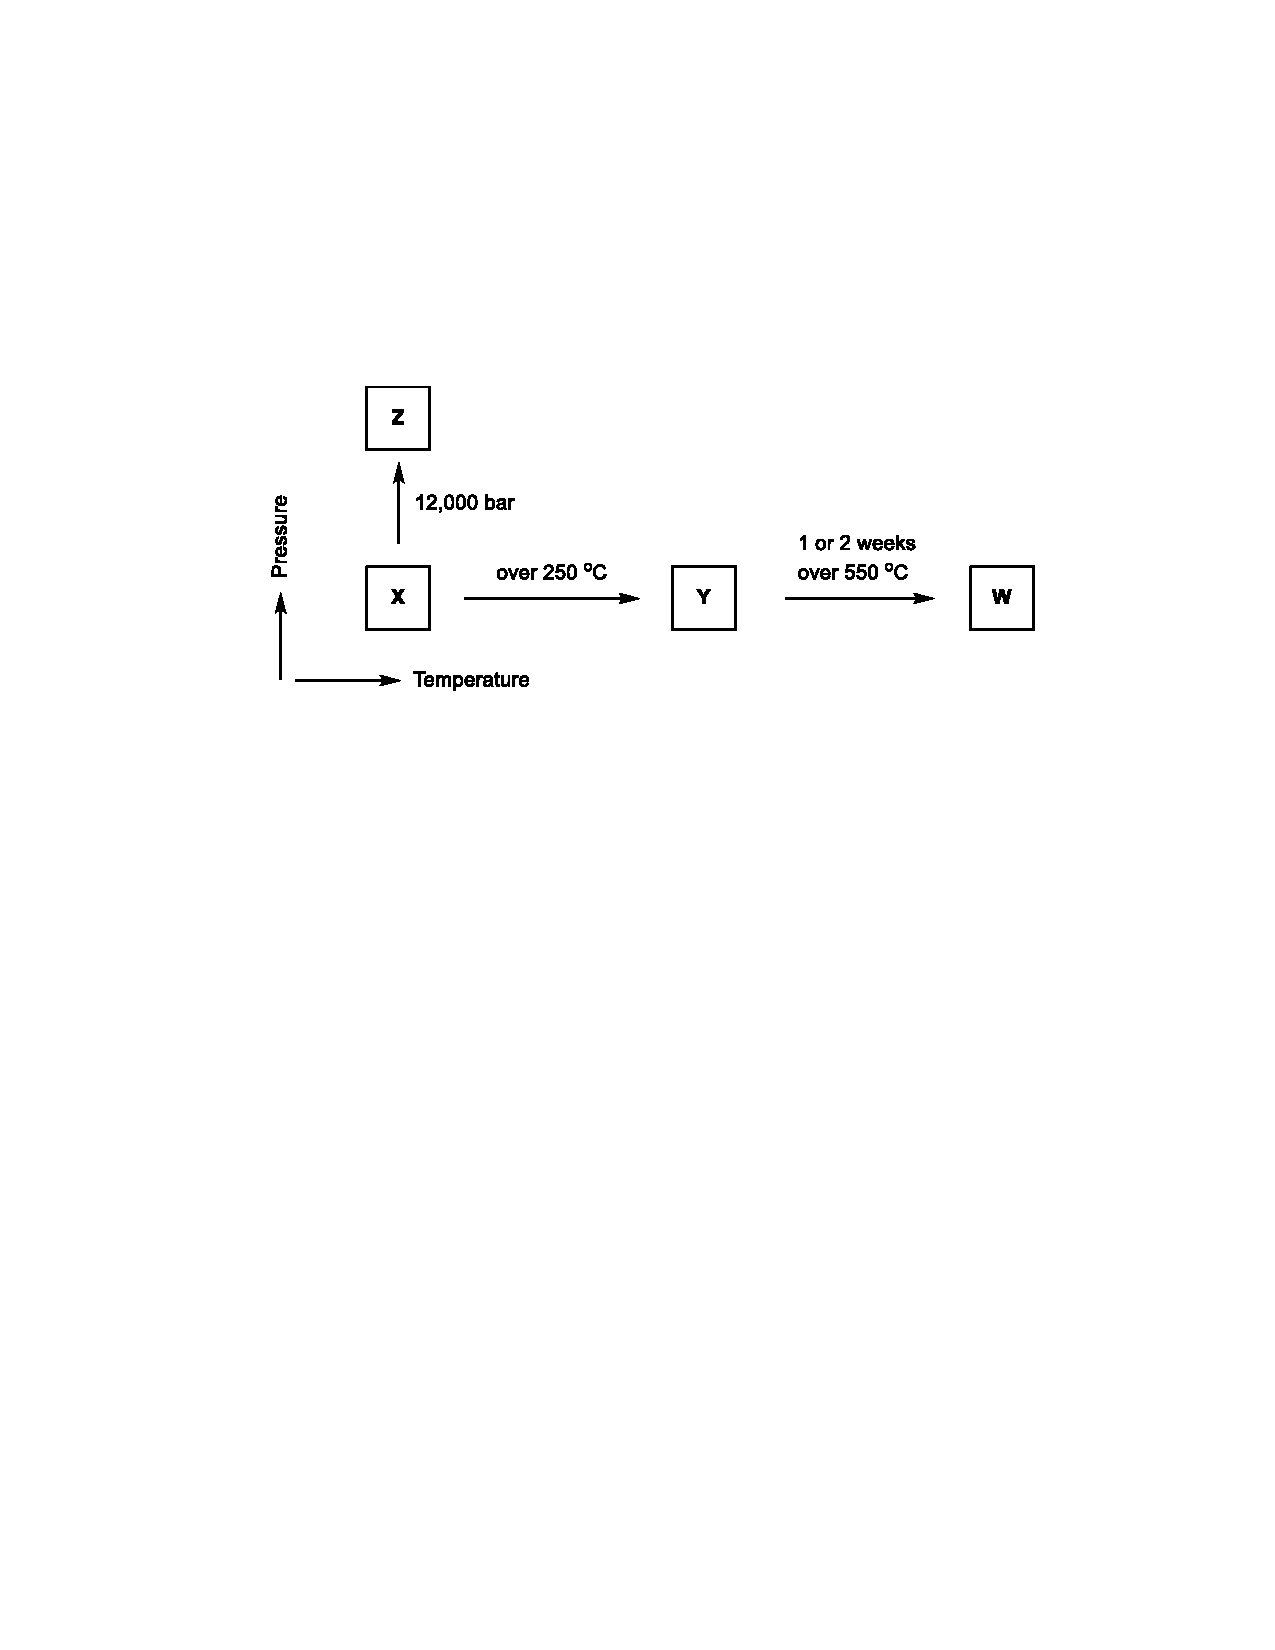
\includegraphics[width=13cm]{./pic/t12-2.pdf}
	\caption*{所有磷同素异形体的转化关系}
\end{figure}

\noindent\textbf{12.1.}
写出\textbf{X},\textbf{Y},\textbf{Z},\textbf{W}分别是哪种磷的同素异形体。

\noindent\textbf{12.2.}
画出\textbf{X},\textbf{Y},\textbf{Z}的结构,绘出\textbf{X}的立体结构。

P\textsubscript{4}可在35 °C附近在空气中点燃得到一种磷的氧化物,因此它保存在水中。当P\textsubscript{4}与不同量的干燥卤素反应时,可得到三卤化磷(PX\textsubscript{3})或五卤化磷(PX\textsubscript{5}),PX\textsubscript{5}也可通过PX\textsubscript{3}与卤素反应得到。五卤化磷可经历两步水化得到酸,磷酰卤可由适量五卤化磷与少量水反应制得,也可由三卤化磷与氧气反应制得。将磷的氧化物投入水中,会产生嘶嘶声,放热,生成酸。P\textsubscript{4}与氢氧化钠或氢氧化钾反应生成主产物磷化氢及副产物磷化钾、磷化钠。磷在氯气中自发燃烧,生成三卤化磷(PX\textsubscript{3})或五卤化磷(PX\textsubscript{5})。

\noindent\textbf{12.3.} 写出下图中化合物\textbf{A-F}的化学式。

\begin{figure}[h]
	\centering
	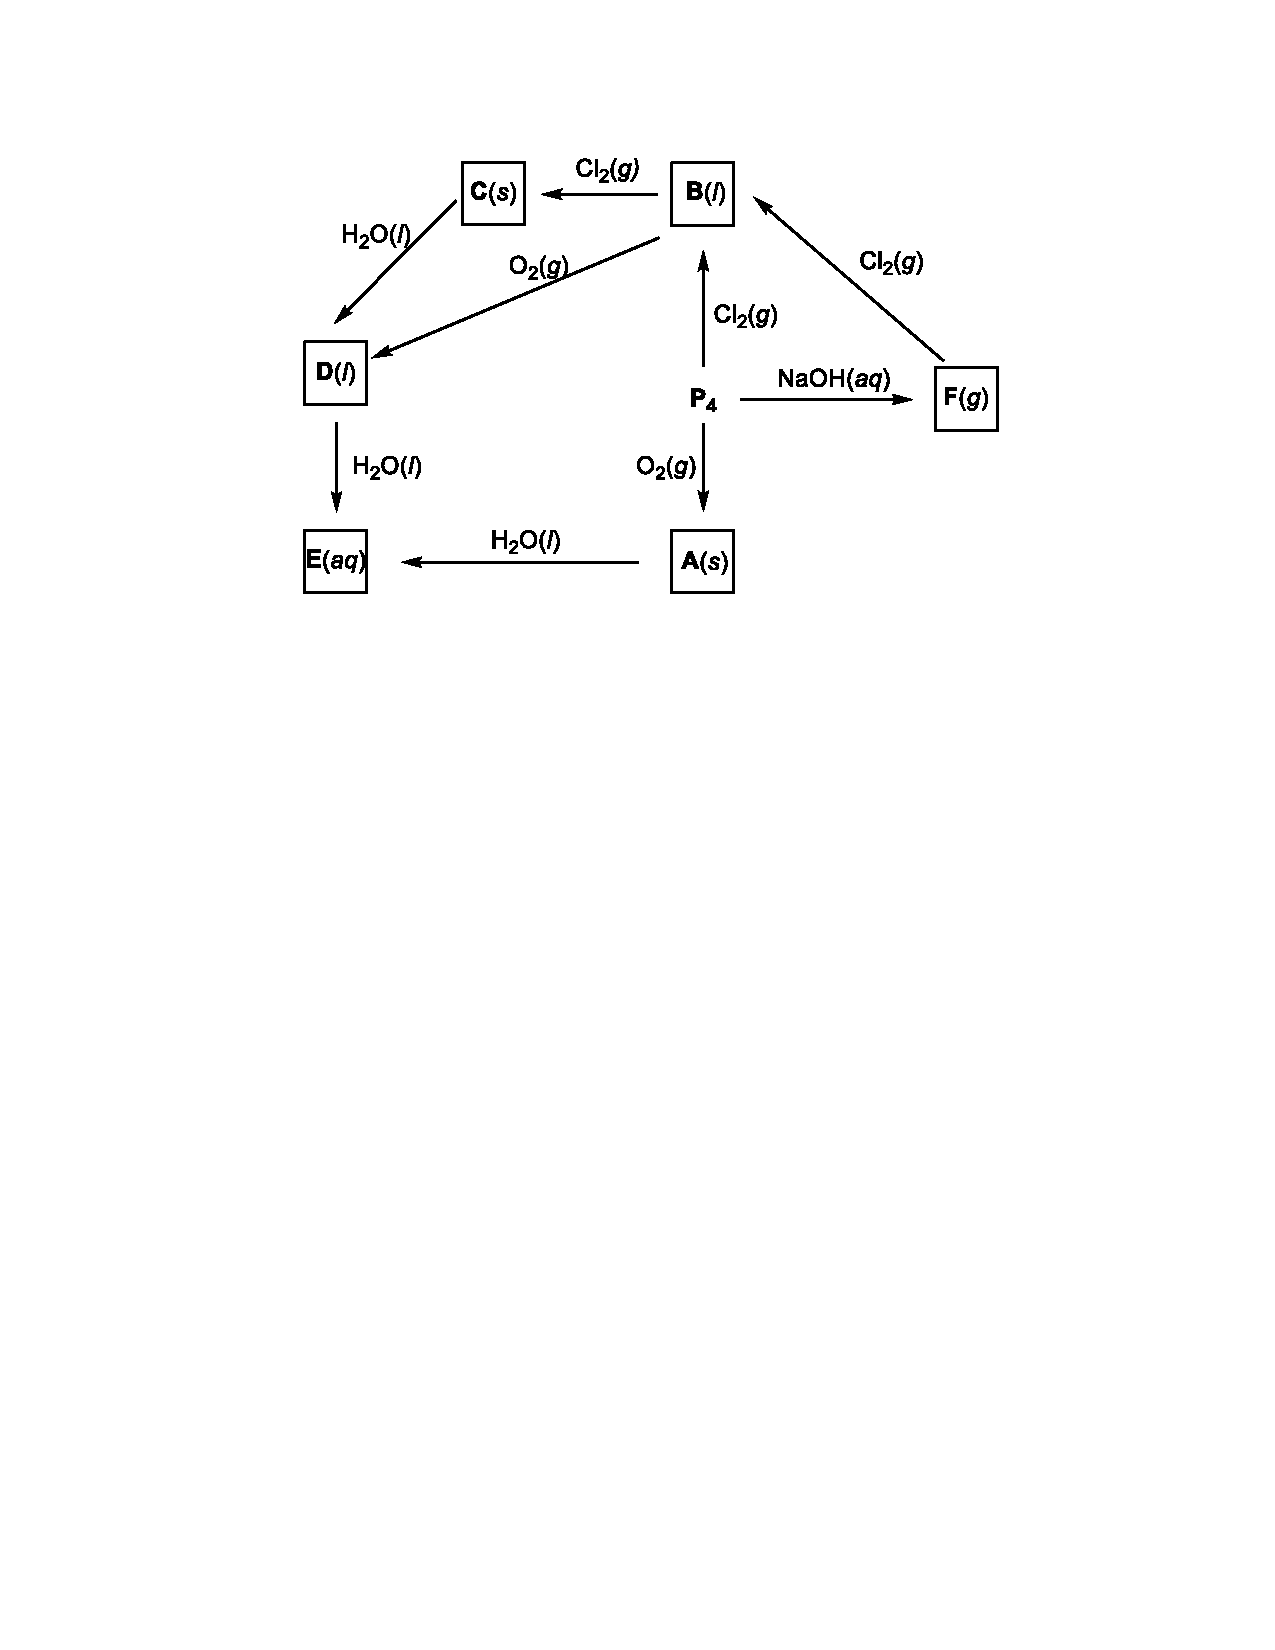
\includegraphics[width=12cm]{./pic/t12-3.pdf}
\end{figure}

磷与过量卤素反应生成如PCl\textsubscript{5}的五配位化合物。如PF\textsubscript{2}Cl\textsubscript{3}的混合五卤化磷由一种卤素与另一种卤素形成的三卤化磷反应制得。

\noindent\textbf{12.4.}
画出PCl\textsubscript{5}和PF\textsubscript{2}Cl\textsubscript{3}的路易斯结构式。

\noindent\textbf{12.5.}
根据VSEPR理论,预测PCl\textsubscript{5}和PF\textsubscript{2}Cl\textsubscript{3}的分子构型。

\noindent\textbf{12.6.}
估计PCl\textsubscript{5}和PF\textsubscript{2}Cl\textsubscript{3}分子的极性。

\noindent\textbf{12.7.} 比较PCl\textsubscript{5}中轴向与赤道面上的P--Cl键键长。

\noindent\textbf{12.8.}
画出PF\textsubscript{2}Cl\textsubscript{3}的杂化方式,预估哪些杂化轨道用于形成轴向与赤道面上的P-X键。

\noindent\textbf{12.9.}
以下是用氢气和白磷合成PH\textsubscript{3}的方程式。利用键能计算反应的$\Delta H$。(单键键能(kJ mol\textsuperscript{-1}),P--P: 213, H--H: 435, P--H: 326)。

$$\ce{P4(g)}+\ce{6H2(g) -> 4 PH3(g)}$$

有机磷化合物是含磷的有机化合物。磷可形成多种氧化态,这些有机磷化合物往往由其中磷主要由磷(V)还是磷(III)构成区别。有机磷化合物被广泛用作亲核试剂和配体,其中两大主要应用为作为Wittig反应的反应物和均相催化剂中的膦配体。它们与卤代烷反应生成膦盐证实了它们的亲电能力十分显著。膦可作为有机合成的亲电催化剂,如Rauhut-Currier反应和Baylis-Hillman反应。

三苯基膦(PPh\textsubscript{3})是一种常见的有机磷化合物,被广泛用于有机化合物和有机金属化合物的合成。将化合物\textbf{1}的丙酮溶液与过量PPh\textsubscript{3}加热回流,会先形成化合物\textbf{2},再形成化合物\textbf{3}。

\begin{figure}[h]
	\centering
	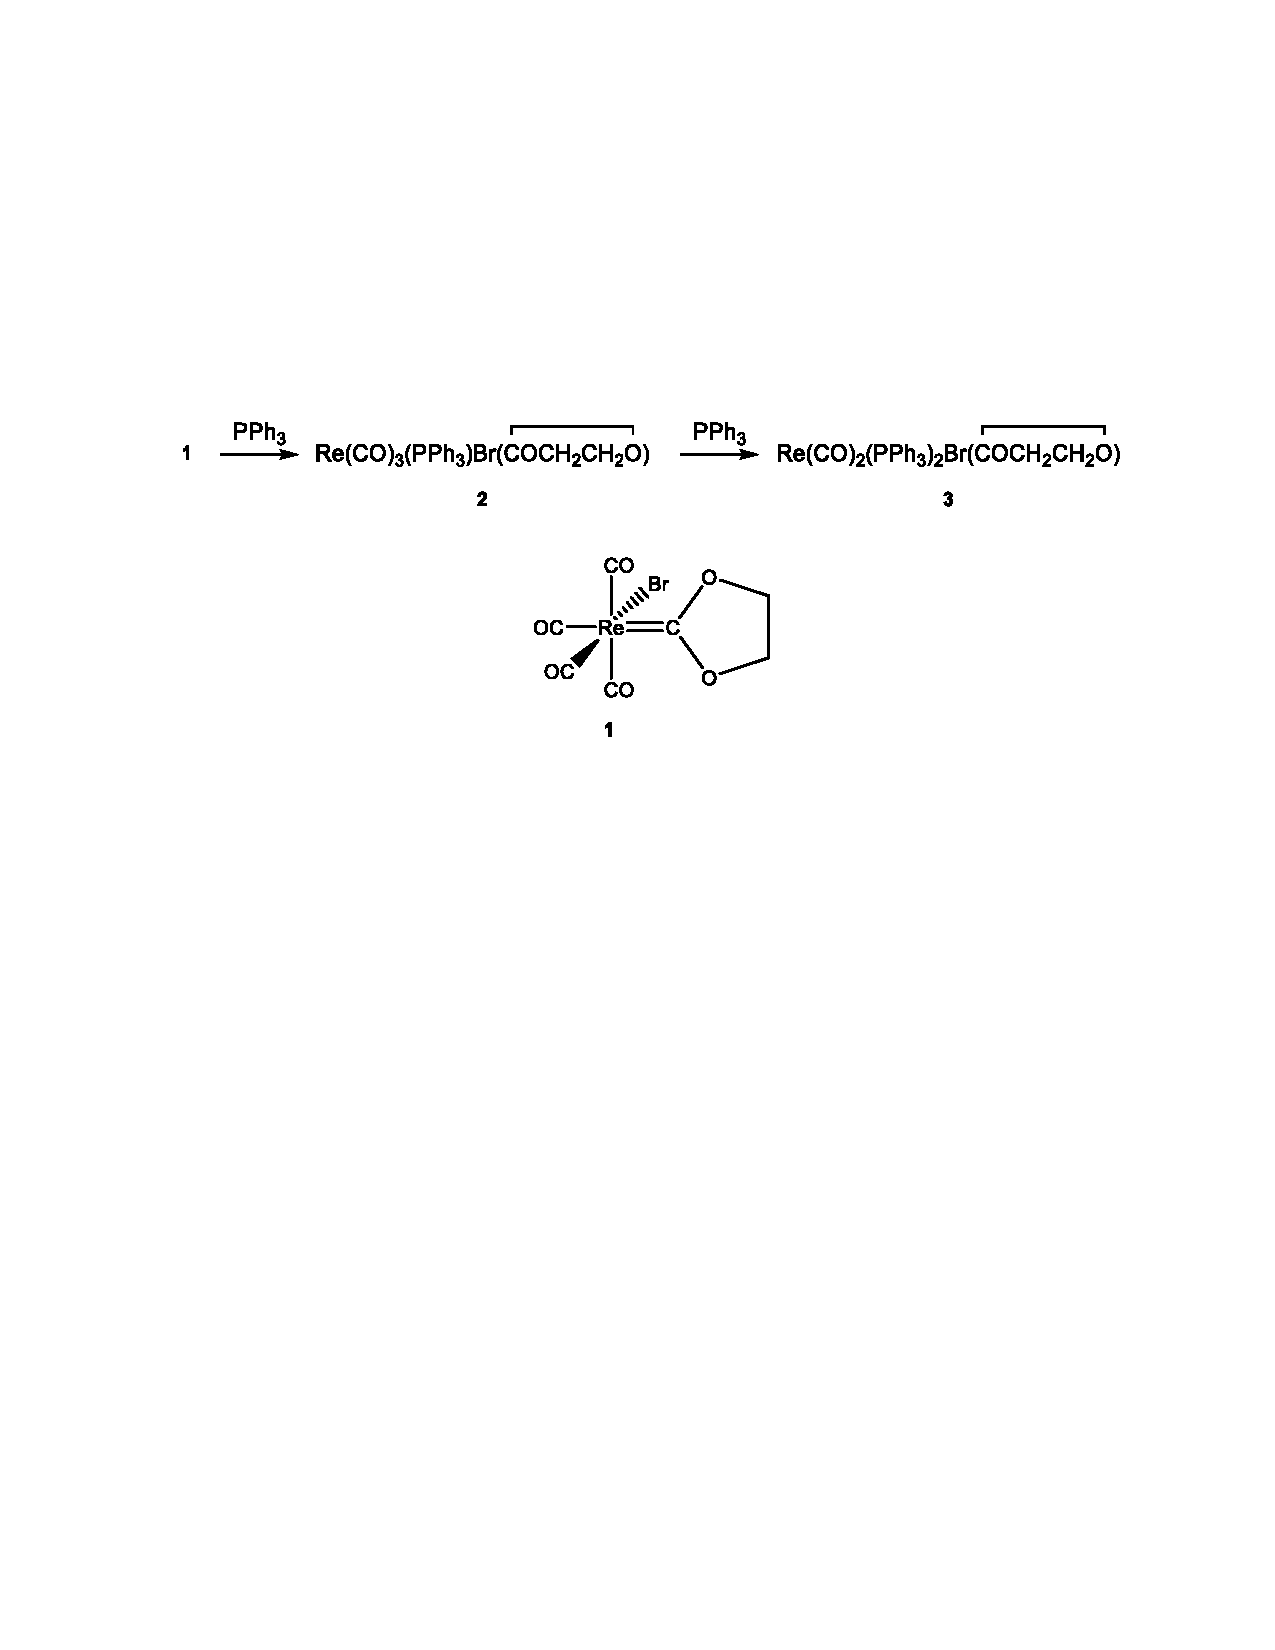
\includegraphics[width=15cm]{./pic/t12-4.pdf}
\end{figure}

化合物1-3的谱学数据列于下表(\textsuperscript{1}H
NMR与\textsuperscript{13}C NMR 数据为相对$\delta$值)

\begin{longtable}[]{@{}llll@{}}
	\toprule
	& \textbf{1} & \textbf{2} & \textbf{3}\tabularnewline
	\midrule
	\endhead
	\begin{minipage}[t]{0.22\columnwidth}\raggedright
		\textsuperscript{1}H NMR\strut
	\end{minipage} & \begin{minipage}[t]{0.22\columnwidth}\raggedright
		4.83 单峰\strut
	\end{minipage} & \begin{minipage}[t]{0.22\columnwidth}\raggedright
		7.62--7.41 (m, 15H)
		
		4.19 (m, 4H)\strut
	\end{minipage} & \begin{minipage}[t]{0.22\columnwidth}\raggedright
		7.70--7.32 (m, 30H)
		
		3.49 (s, 4H)\strut
	\end{minipage}\tabularnewline\midrule
	\begin{minipage}[t]{0.22\columnwidth}\raggedright
		\textsuperscript{13}C NMR\strut
	\end{minipage} & \begin{minipage}[t]{0.22\columnwidth}\raggedright
		224.3
		
		187.2
		
		185.3
		
		184.0
		
		73.3\strut
	\end{minipage} & \begin{minipage}[t]{0.22\columnwidth}\raggedright
		231.0
		
		194.9
		
		189.9
		
		188.9
		
		129.0--134.7 (多峰)
		
		72.2\strut
	\end{minipage} & \begin{minipage}[t]{0.22\columnwidth}\raggedright
		237.1
		
		201.8
		
		193.8
		
		127.7--134.0 (多峰)
		
		68.80\strut
	\end{minipage}\tabularnewline\midrule
	\begin{minipage}[t]{0.22\columnwidth}\raggedright
		IR\strut
	\end{minipage} & \begin{minipage}[t]{0.22\columnwidth}\raggedright
		\strut
	\end{minipage} & \begin{minipage}[t]{0.22\columnwidth}\raggedright
		2038 cm\textsuperscript{--1}
		
		1958 cm\textsuperscript{--1}
		
		1906 cm\textsuperscript{--1}\strut
	\end{minipage} & \begin{minipage}[t]{0.22\columnwidth}\raggedright
		1944 cm\textsuperscript{--1}
		
		1860 cm\textsuperscript{--1}\strut
	\end{minipage}\tabularnewline\midrule
	MS (m/z) & & 684.5 & 919.7\tabularnewline
	\bottomrule
\end{longtable}


\noindent\textbf{12.10.} 画出化合物2和3的结构。

\noindent 提示:化合物\textbf{1}的在224.3 ppm的\textsuperscript{13}C
NMR信号与卡宾碳的信号类似;184、202 ppm的信号与羰基信号一致;在73.3
ppm的信号是典型的双氧碳烯配体中CH\textsubscript{2}CH\textsubscript{2}桥的信号。

\noindent\textbf{12.11.}
指出化合物\textbf{2}更有可能是面式(\emph{fac})还是经式(\emph{mer})异构体。

\noindent 提示:化合物\textbf{2}的红外光谱中观察到三个等强度羰基振动峰。卡宾配体的质子在\textsuperscript{1}H
NMR表现为多重峰。

\noindent\textbf{12.12.}
指出化合物\textbf{3}更有可能是顺式(\emph{cis})还是反式(\emph{trans})异构体?

\noindent 提示:化合物\textbf{3}的红外光谱中两个几乎等强度的羰基振动峰位于1944、1860
cm\textsuperscript{-1}。\textsuperscript{31}P NMR显示一个单峰信号。

尽管许多有机磷化合物,如Sarin,Soman,VX在室温下为液体,它们仍被称为``神经毒气''。1997年,签署了化学武器协定的国家,同意禁止化学武器,并在2012年之前销毁了化学武器及其生产装置。Sarin在室温下可被Na\textsubscript{2}CO\textsubscript{3}水溶液破坏,生成NaF和一种有机磷化合物的钠盐。VX的水化实现起来则更为困难,它在室温下与NaOH缓慢反应,在360 K时需反应数小时。

\begin{figure}[h]
	\centering
	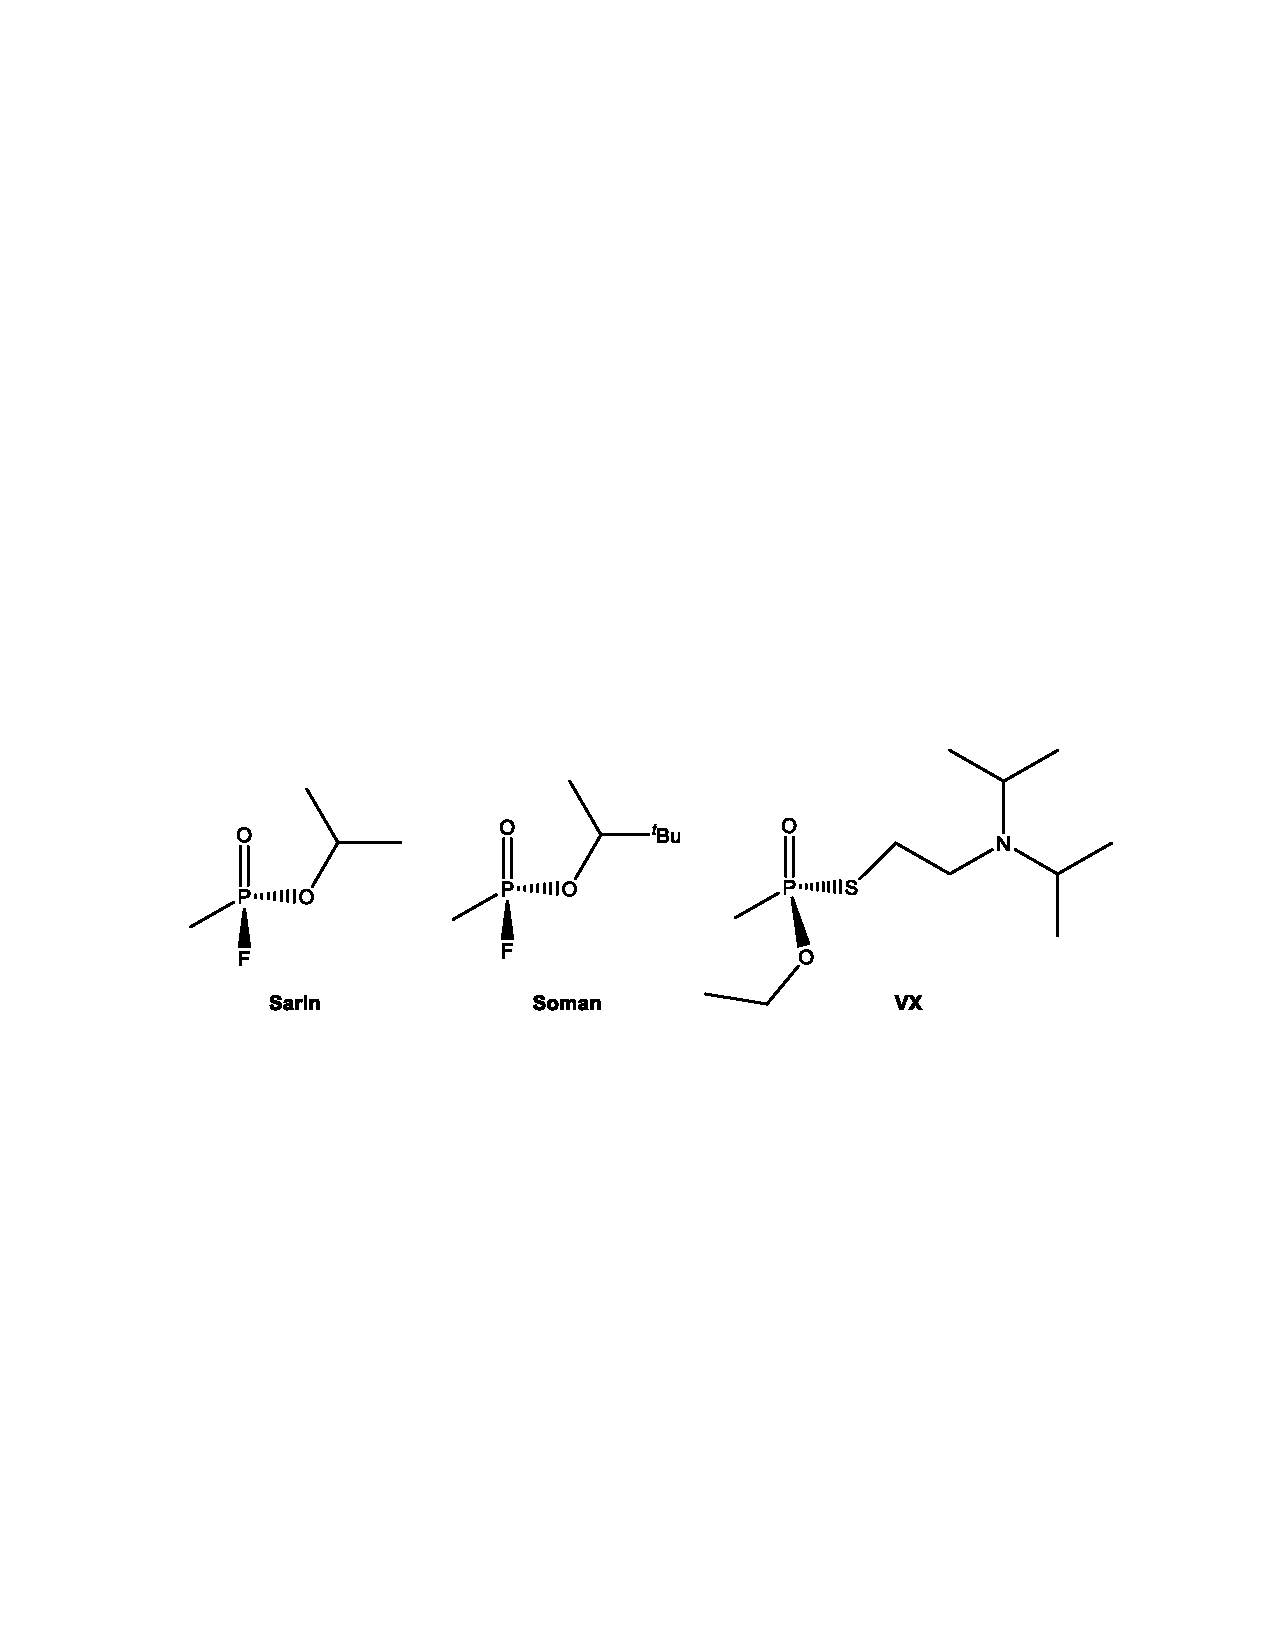
\includegraphics[width=15cm]{./pic/t12-5.pdf}
\end{figure}

\noindent\textbf{12.13.} 指出以下反应生成的有机磷化合物的盐的化学式。

\begin{figure}[h]
	\centering
	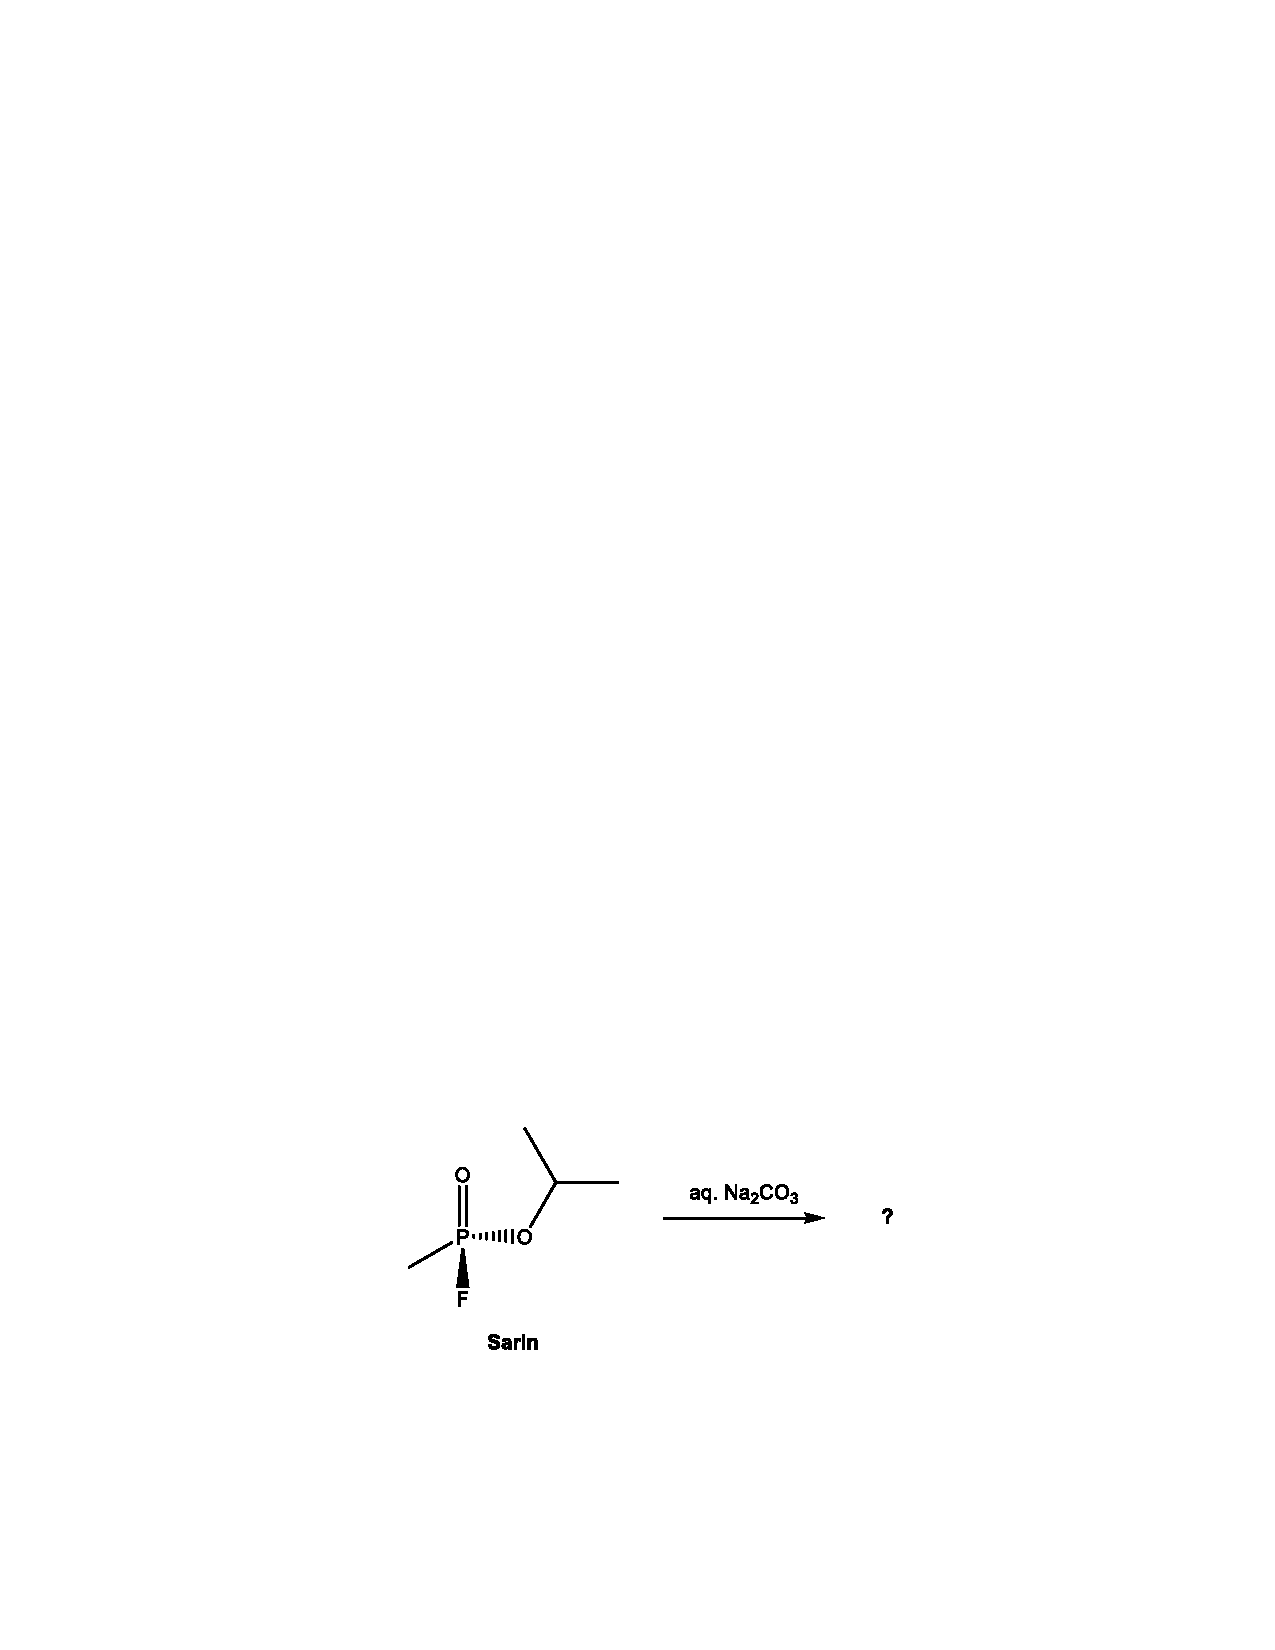
\includegraphics[width=8cm]{./pic/t12-6.pdf}
\end{figure}

两种具有八面体结构的铬配合物含有配体CO,PF\textsubscript{3},PCl\textsubscript{3}。在八面体配合物中,配合物的分子轨道由六个$\sigma$配体每个提供2个电子时,称作$\sigma$配位;当配体有空的\textit{p},\textit{d}或$\pi^*$轨道时,$\pi$配位也是可能的。配体如CO、CN\textsuperscript{-}和膦是$\pi$受体,具有可以与金属\textit{d}轨道形成$\pi$键的能力。在大多数情况下,反馈$\pi$键占据主导地位,电子云密度由中心流向配体,$\pi$配位可以影响羰基、膦配体的键能、键长。

考虑$\pi$配位作用,回答下两个小问。

\noindent\textbf{12.14.}
哪个配合物中的C--O键键长更短,Cr(CO)\textsubscript{5}(PF\textsubscript{3})还是Cr(CO)\textsubscript{5}(PCl\textsubscript{3})?

\noindent\textbf{12.15.}
在红外光谱中,哪个配合物的C--O键振动能量更高,Cr(CO)\textsubscript{5}(PF\textsubscript{3})还是Cr(CO)\textsubscript{5}(PCl\textsubscript{3})?


\newpage
\mysection{第14题\  抗癌的铂络合物}
\begin{figure}[h]
	\centering
	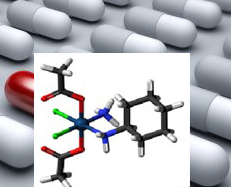
\includegraphics[width=7cm]{./pic/t14-1.png}
\end{figure}

基于金属药物的药用无机化学被广泛定义为与金属离子和金属络合物及其临床应用有关的研究领域。这是从抗癌药顺铂的发现发展起来的一个新的研究领域。顺铂,顺二氯二氨铂(II),是一种黄色粉末,也是一种抗癌药物。其广泛用于治疗多种肿瘤,尤其是睾丸,卵巢,头和颈部的肿瘤。

顺铂的合成始于K\textsubscript{2}[PtCl\textsubscript{4}],自100多年前发表以来,已经历了几处改进。主要问题是杂质的出现和副产物反铂的形成。如今合成路线主要基于Dhara在1970年代发表的方法。在初始步骤中,K\textsubscript{2}[PtCl\textsubscript{4}]与过量的KI反应,然后将铂络合物转化为碘类似物\textbf{A}。随后,将NH\textsubscript{3}加入化合物\textbf{A}中,并通过配体交换形成化合物\textbf{B},其中两个NH\textsubscript{3}配体与两个碘配体交换。\textbf{B}是黄色固体,将其过滤,干燥并与AgNO\textsubscript{3}的水溶液混合。可以滤出不溶的AgI,形成顺式二氨二水合铂硝酸盐\textbf{C};然后将过量的KCl加入\textbf{C}溶液中,得到顺铂\textbf{D}。

合成的成功取决于碘配体的强反位效应。在平面四方配合物中与离去基团处在反式的旁观配体\textbf{T}影响取代的速度。这种现象称为反位效应。关键是强的$\sigma$给体配体或$\pi$受体配体极大地促进了反式的配体取代。反位效应遵循以下顺序。

作为$\sigma$给体的\textbf{T}:OH\textsuperscript{−}< NH\textsubscript{3}<Cl\textsuperscript{−}<Br\textsuperscript{−}<CN\textsuperscript{−},CH\textsubscript{3}\textsuperscript{−}<I\textsuperscript{−}<SCN\textsuperscript{−},PR\textsubscript{3},H\textsuperscript{−}

对于$\pi$受体的\textbf{T}:Br\textsuperscript{‑}<I\textsuperscript{−}<NCS\textsuperscript{−}<NO\textsubscript{2}\textsuperscript{−}<CN\textsuperscript{−}<CO,C\textsubscript{2}H\textsubscript{4}

\begin{figure}[h]
	\centering
	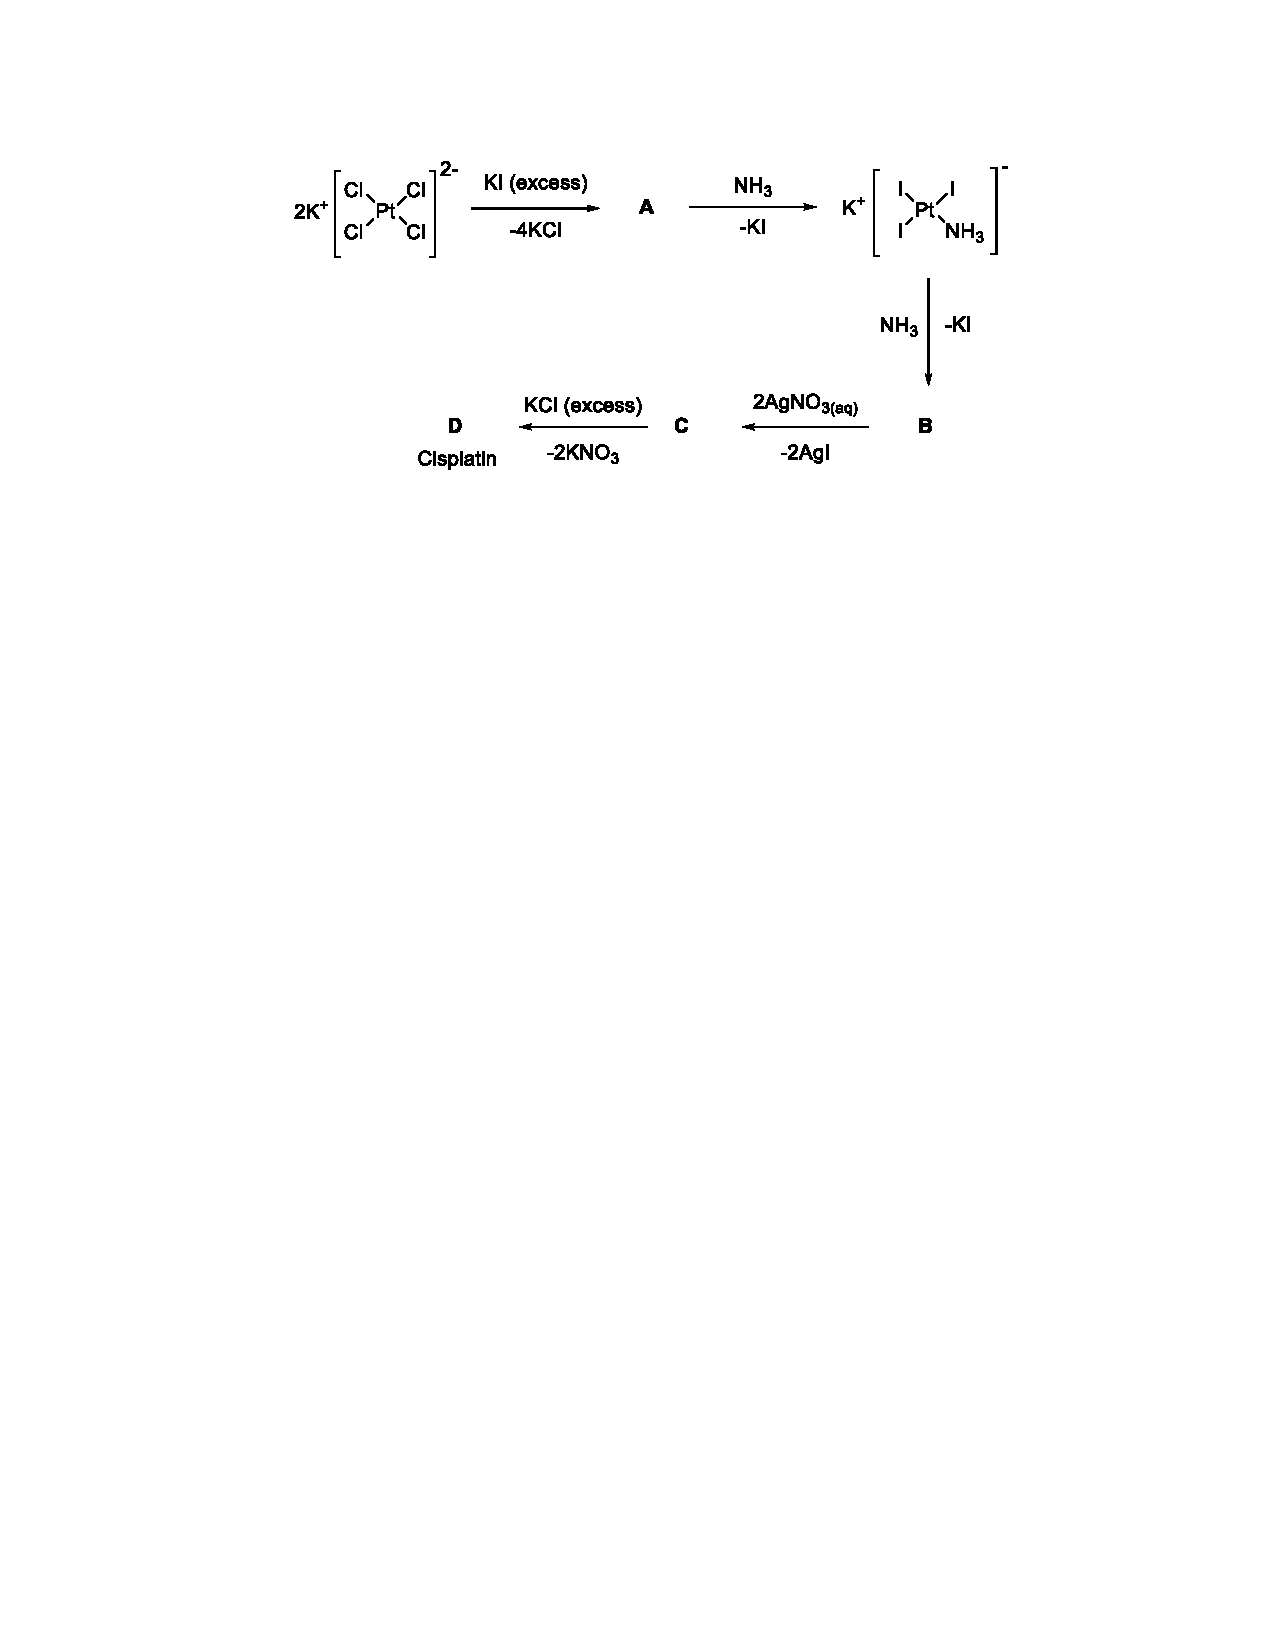
\includegraphics[width=13cm]{./pic/t14-2.pdf}
\end{figure}

\noindent\textbf{14.1.} 写出\textbf{A}-\textbf{D}的分子式

\noindent\textbf{14.2.} 画出\textbf{A}-\textbf{D}的分子结构

\noindent\textbf{14.3.} 化合物\textbf{D}是极性的吗?

\noindent\textbf{14.4.} 运用晶体场理论,画出顺铂\textbf{D}的\textit{d}轨道分裂图并展示电子分配示意图。

\noindent\textbf{14.5.} 确定络合物\textbf{A}的磁性。

铂络合物与DNA结合并引起交联,从而触发程序性细胞死亡(细胞凋亡)。然而,平面四方结构的另一几何异构体反铂,反式二氯二氨合铂(II)\textbf{F},对癌症的治疗无效。反铂是从[Pt(NH\textsubscript{3})\textsubscript{4}]\textsuperscript{2+}开始合成的,然后陆续添加二个Cl\textsuperscript{−}配体以形成反铂\textbf{F},如下图所示。

\begin{figure}[h]
	\centering
	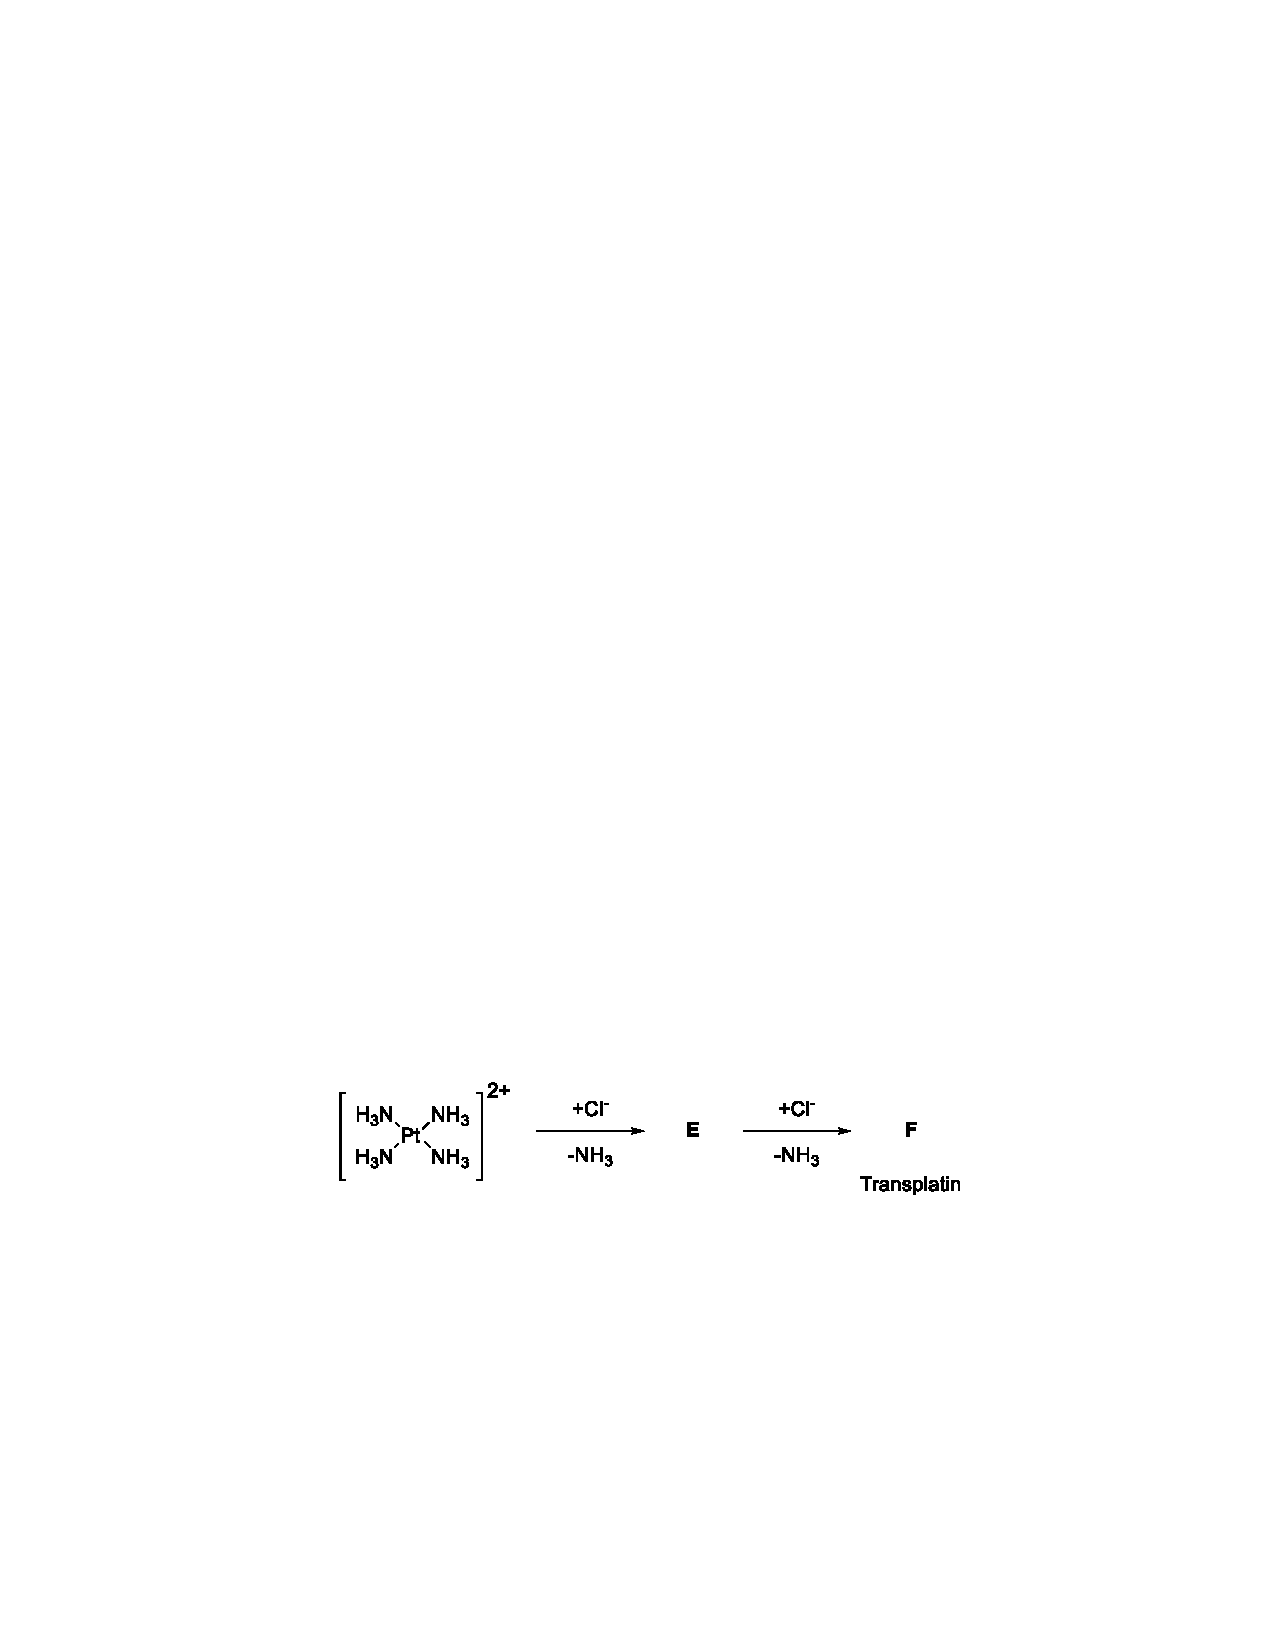
\includegraphics[width=11cm]{./pic/t14-3.pdf}
\end{figure}

\noindent\textbf{14.6.} 画出\textbf{E}和\textbf{F}的分子结构

最重要的一类抗肿瘤药顺铂,卡铂(carboplatin)和奥沙利铂(oxaliplatin)作为二胺合铂(II)被广泛用于化学疗法中,以治疗各种癌症。

\begin{figure}[h]
	\centering
	\includegraphics[width=8cm]{./pic/t14-4.pdf}
\end{figure}

但是,这些药物的治疗指数相对较窄。它们的使用经常受到严重毒性和抗药性的困扰,这导致疾病进展。最近,氧铂(oxoplatin),异丙铂(iproplatin),奥马铂(ormaplatin)和沙铂(satraplatin)是临床上已经使用的(氧铂)或试验中的铂络合物。

\begin{figure}[h]
	\centering
	\includegraphics[width=13cm]{./pic/t14-5.pdf}
\end{figure}

\noindent\textbf{14.7.}
所有配合物有相同的几何结构和对于Pt中心原子的氧化数。写出Pt的氧化数和配合物的几何构型。

\noindent\textbf{14.8.} 哪一个Pt络合物,顺铂还是沙铂,对于取代反应更动力学惰性?

\noindent\textbf{14.9.}
奥沙铂是[Pt(NH\textsubscript{3})\textsubscript{2}Cl\textsubscript{2}(OH)\textsubscript{2}]的一个异构体。画出所有的立体异构体并指明哪些有手性。

铂络合物(氧铂,异丙铂,奥马铂和沙铂)可以被认为是前体药,其主要在细胞内被生物还原剂(如硫醇,抗坏血酸和谷胱甘肽(GSH))激活以杀死癌细胞。

例如,在一项研究中,癌细胞(A2780,A2780cisR和HT-29)的水溶液提取物可还原具有与沙铂相似结构的\textit{cis},\textit{trans},\textit{cis}-[PtCl\textsubscript{2}(OCOCH\textsubscript{3})\textsubscript{2}(NH\textsubscript{3})\textsubscript{2}](\textbf{G},前药)产生顺铂(\textbf{D},药物)和游离乙酸根离子,如下所示。

\begin{figure}[h]
	\centering
	\includegraphics[width=8cm]{./pic/t14-6.pdf}
\end{figure}

\noindent\textbf{14.10.} 画出\textbf{G}的分子结构

\noindent\textbf{14.11.} 画出\textbf{G}中金属离子的\textit{d}轨道分裂并写出电子排布。

\noindent\textbf{14.12.} \textbf{G}是顺磁性还是反磁性的?

络合物\textbf{G}结晶成单斜晶体,其晶胞参数为:$a=14.9973$,$b=8.57220$,$c=11.1352$ \AA,$\beta=126.7690^{\circ} $,晶胞中的分子数$Z=4$,$M=436.16\ $g mol\textsuperscript{−1}(配合物在晶体结构中有一个水分子)。

\noindent\textbf{14.13.} 计算化合物的密度$\rho$。提示:单斜晶胞的体积为$V=a\times b\times c\times \sin\beta$



\newpage
\mysection{第15题\  盐中的钠化合物}
土耳其的盐湖盆地对于保护生物多样性非常重要,根据国际标准被归类为湿地。它也是土耳其保有鸟类最多的湖泊之一。有鸟类85种,昆虫129种(其中4种是特有的),15种哺乳动物和38种特有的植物。该湖满足了土耳其约40\%的食盐需求(作为食用盐)。盐湖中的盐是由气象水排入地下并融化先前形成的盐穹顶,并沿构造线携带它们而形成的。盐湖中的盐生产是通过在阳光下蒸发湖水来完成的。我们利用太阳能通过池式系统制盐。

\begin{figure}[h]
	\centering
	\includegraphics[width=10cm]{./pic/t15-1.jpg}
	\caption*{盐湖}
\end{figure}

食用盐是最常见的家用化学品之一。它是97\%到99\%的氯化钠,它是化学式为NaCl的离子化合物,代表钠和氯离子的比例为1:1。NaCl是最影响海水和许多多细胞生物体细胞外液盐度的化合物。食用盐的可食用形式通常用作调味品和食品防腐剂。钠的第二个主要应用是在亚冰冻天气中,用氯化物给道路除冰。大量氯化钠还用于许多工业过程中,例如氯碱工业和纯碱工业以及其他工业用途:水软化,医药,农业,消防和清洁剂。NaCl直接或间接用于生产许多钠化合物。世界上大部分产量都为钠化合物。下图显示了从NaCl制备一些钠化合物的方法。

\begin{figure}[h]
	\centering
	\includegraphics[width=14cm]{./pic/t15-2.pdf}
	\caption*{从NaCl开始制备一些钠化合物。}
\end{figure}

\noindent\textbf{15.1.} 写出\textbf{A}-\textbf{G}的分子式

碳酸钠(Na\textsubscript{2}CO\textsubscript{3},苏打粉),主要用于制造玻璃。它主要来源于天然产物,例如天然碱,Na\textsubscript{2}CO\textsubscript{3}·NaHCO\textsubscript{3}·$n$H\textsubscript{2}O。其主要可通过NaCl,CaCO\textsubscript{3},NH\textsubscript{3}用一个比利时化学家Ernest Solvay在1863年发明的方法生产。关键步骤包括NH\textsubscript{3}(g)和CO\textsubscript{2}(g)在饱和NaCl(aq)中反应。在所有可能从混合物结晶的离子型化合物中(NaCl,NH\textsubscript{4}Cl,NaHCO\textsubscript{3},NH\textsubscript{4}HCO\textsubscript{3}),溶解度最小的是碳酸氢钠(NaHCO\textsubscript{3})。它通过过滤分离出来,然后通过加热转化为碳酸钠(Na\textsubscript{2}CO\textsubscript{3})。根据解释,

\noindent\textbf{15.2.} 配平下面的方程式

$\ce{NaCl(aq) + CO2(g) + NH3(g) + H2O ->}$

$\ce{2NaHCO3(s) ->[\Delta]}$

\noindent\textbf{15.3.}
使用CaCO\textsubscript{3}(石灰石),你怎样才能获得你想要的CO\textsubscript{2}气体来生产NaHCO\textsubscript{3}?

\noindent\textbf{15.4.}
写出CaCO\textsubscript{3}的包含所有共振式的Lewis结构,并标出每个原子的形式电荷。

\noindent\textbf{15.5.}
描述CO$_3^{2-}$的分子几何结构并提出中心原子合理的杂化方式。

\noindent\textbf{15.6.}
按照键长增长的顺序排列CO$_3^{2-}$,CO,CO\textsubscript{2}

NaCl结晶为面心立方(fcc)结构。NaCl的密度为2180
kg m\textsuperscript{−3},Na\textsuperscript{+}的离子半径为99pm。

\noindent\textbf{15.7.} 在晶胞中有多少原子?什么原子占据八面体空隙?

\noindent\textbf{15.8.}
计算NaCl的晶胞长度和Cl\textsuperscript{−}的离子半径(用pm)

碱金属与氧气快速反应,生成几种不同的离子型氧化物。在适当的条件下,通常通过仔细控制氧气,每种碱金属都能生成氧化物M\textsubscript{2}O。
锂与过量氧气反应生成\textbf{A}和少量的\textbf{B}。钠与过量的氧气反应生成大部分\textbf{C}和少量\textbf{D}。钾,铷和铯反应与过量的氧气形成\textbf{E},\textbf{F}和\textbf{G}。

\noindent\textbf{15.9.} \textbf{A}-\textbf{G}是哪些常见的金属氧化物?

\noindent\textbf{15.11.} 画出过氧和超氧离子的分子轨道能级图并比较它们的键长和能量。

当LiClO\textsubscript{4},NaClO\textsubscript{4}和KClO\textsubscript{4}从水溶液结晶时,它们可能包含或不包含称为结晶水的水分子作为固体结构的一部分,尽管没有简单的规则可以确定地预测离子在固态中是否保留其全部或部分水化球,具有高电荷密度的阳离子倾向于将其全部或部分水化球保留在固态中。当阳离子具有低电荷密度时,它们往往会失去其水合球;因此,它们倾向于形成无水盐。Li\textsuperscript{+},Na\textsuperscript{+}和K\textsuperscript{+}的离子半径分别为76 pm,102 pm和138 pm。

\noindent\textbf{15.12.} 计算这些离子的电荷密度(单位用C mm\textsuperscript{−3})

\noindent\textbf{15.13.} 哪种高氯酸盐最易形成无水化合物?


\newpage
\mysection{第25题\  分光光度法测定抗组胺药}

分光光度法是用于确定药物分子的简单,快速和准确的方法。该方法基于两种试剂之间形成复合物。许多复合物是有色的,并在可见光区域有吸收。因此可以用分光光度法测定它们。

抗组胺药物\textbf{D}作为给电子基团,与$\pi$-受体\textbf{S}复合。所得的复合物在最大吸收(460 nm)处记录的吸光度与药物浓度线性相关,具有良好的相关系数。
$$
\begin{aligned}
\mathrm D+\mathrm S\rightleftharpoons\mathrm {DS}\\
K=\frac{[\mathrm{DS}]}{[\mathrm D][\mathrm S]}\\
\end{aligned}
$$
其中\([\mathrm{DS}]\),\([\mathrm D]\)与\([\mathrm S]\)分别代表\textbf{DS}复合物,\textbf{D}与\textbf{S}的平衡浓度。
\[
c_{\mathrm D}=[\mathrm D]+[\mathrm {DS}]
\] 
其中\(c_{\mathrm D}\)是药物的总浓度。

只有所形成的\textbf{DS}络合物可以吸收光的波长下,以下表达式成立:

 \[
A=\varepsilon_{\mathrm{DS}}l[\mathrm{DS}]
\] 
其中\(l\)是吸收池长度。

可以使用Benesi--Hildebrand方程来计算络合物的结合平衡常数,该方程取决于实验条件,其中一种组分应大量过量,以使其浓度不会随复合物的形成而改变。

\[
\frac{c_{\mathrm D}}{A_{\mathrm{DS}}}=\frac{1}{\varepsilon_{\mathrm{DS}}}+\frac{1}{\varepsilon_{\mathrm{DS}}K}\times\frac{1}{c_{\mathrm S}}
\]
其中\(c_{\mathrm S}\)与\(c_{\mathrm D}\)是\textbf{S}与\textbf{D}的总浓度。\(A_{\mathrm{DS}}\)是复合物的吸光度,\(\varepsilon_{\mathrm{DS}}\)是复合物的摩尔吸光系数,\(K\)是平衡常数。

\begin{figure}[h]
	\centering
	\includegraphics[width=12cm]{./pic/t25-1.pdf}
\end{figure}

\noindent\textbf{25.1.} 考虑在25
°C下记录的Benesi--Hildebrand图,给出复合物生成的平衡常数和复合物的摩尔吸光系数。


\noindent\textbf{25.2.}
\textbf{D}与\textbf{S}的起始浓度是9×10\textsuperscript{−5} mol
L\textsuperscript{−1},计算平衡时复合物形成的百分数。\textbf{D}与\textbf{S}在复合的时候比例为1:1。

\noindent\textbf{25.3.} 计算25 °C下的\(\Delta_rG^\ominus\),单位为kJ
mol\textsuperscript{−1}。

通过改变温度(25、45和60 °C)研究\textbf{D}与\textbf{S}的络合动力学。该表给出了在不同温度下的络合速率常数。

\begin{longtable}[]{@{}llll@{}}
	\toprule
	$T$ (°C) &25&45&60 \tabularnewline
	$k$ (min\textsuperscript{--1}) & 0.0200 &0.0504&0.0944\tabularnewline
	\bottomrule
\end{longtable}

\noindent\textbf{25.4.} 计算活化能\(E_a\)。

\noindent\textbf{25.5.}
已知\(k_{\mathrm{TST}}=\frac{k_{\mathrm BT}}{h}e^{-\frac{\Delta G^\ddag}{RT}}\),计算25 °C下的活化焓\(\Delta H^\ddag\),活化熵\(\Delta S^\ddag\)以及活化自由能\(\Delta G^\ddag\)。
(译注:原文为自由活化焓\(\Delta G^\ddag\))



\mychapter{实验试题}


\end{document}                          % The required last line